\documentclass[11pt]{article}

%%%%%%%%%%%%%%Include Packages%%%%%%%%%%%%%%%%%%%%%%%%%%
\usepackage{xcolor}
\usepackage{mathtools}
\usepackage[a4paper, total={6in, 8in}, margin=1.25in]{geometry}
\usepackage{amsmath}
\usepackage{amssymb}
\usepackage{paralist}
\usepackage{rsfso}
\usepackage{amsthm}
\usepackage{wasysym}
\usepackage[inline]{enumitem}   
\usepackage{hyperref}
\usepackage{tocloft}
\usepackage{wrapfig}
\usepackage{titlesec}
\usepackage{colortbl}
\usepackage{stackengine} 
%%%%%%%%%%%%%%%%%%%%%%%%%%%%%%%%%%%%%%%%%%%%%%%%%%%%%%%%


%%%%%%%%%%%%%%%Chapter Setting%%%%%%%%%%%%%%%%%%%%%%%%%%
\definecolor{gray75}{gray}{0.75}
\newcommand{\hsp}{\hspace{20pt}}
\titleformat{\chapter}[hang]{\Huge\bfseries}{\thechapter\hsp\textcolor{gray75}{$\mid$}\hsp}{0pt}{\Huge\bfseries}
%%%%%%%%%%%%%%%%%%%%%%%%%%%%%%%%%%%%%%%%%%%%%%%%%%%%%%%%

%%%%%%%%%%%%%%%%%Theorem environments%%%%%%%%%%%%%%%%%%%
\newtheoremstyle{break}
  {\topsep}{\topsep}%
  {\itshape}{}%
  {\bfseries}{}%
  {\newline}{}%
\theoremstyle{break}
\theoremstyle{break}
\newtheorem{axiom}{Axiom}
\newtheorem{thm}{Theorem}[section]
\renewcommand{\thethm}{\arabic{section}.\arabic{thm}}
\newtheorem{lem}{Lemma}[thm]
\newtheorem{prop}[lem]{Proposition}
\newtheorem{corL}{Corollary}[lem]
\newtheorem{corT}[lem]{Corollary}
\newtheorem{defn}{Definition}[corL]
\newenvironment{indEnv}[1][Proof]
  {\proof[#1]\leftskip=1cm\rightskip=1cm}
  {\endproof}
%%%%%%%%%%%%%%%%%%%%%%%%%%%%%%%%%%%%%%%%%%%%%%%%%%%%%%


%%%%%%%%%%%%%%%%%%%%%%%Integral%%%%%%%%%%%%%%%%%%%%%%%
\def\upint{\mathchoice%
    {\mkern13mu\overline{\vphantom{\intop}\mkern7mu}\mkern-20mu}%
    {\mkern7mu\overline{\vphantom{\intop}\mkern7mu}\mkern-14mu}%
    {\mkern7mu\overline{\vphantom{\intop}\mkern7mu}\mkern-14mu}%
    {\mkern7mu\overline{\vphantom{\intop}\mkern7mu}\mkern-14mu}%
  \int}
\def\lowint{\mkern3mu\underline{\vphantom{\intop}\mkern7mu}\mkern-10mu\int}
%%%%%%%%%%%%%%%%%%%%%%%%%%%%%%%%%%%%%%%%%%%%%%%%%%%%%%



\newcommand{\R}{\mathbb{R}}
\newcommand{\N}{\mathbb{N}}
\newcommand{\Z}{\mathbb{Z}}
\newcommand{\Q}{\mathbb{Q}}
\newcommand{\C}{\mathbb{C}}
\newcommand{\T}{\mathcal{T}}
\newcommand{\M}{\mathcal{M}}
\newcommand{\Symm}{\text{Symm}}
\newcommand{\Alt}{\text{Alt}}
\newcommand{\Int}{\text{Int}}
\newcommand{\Bd}{\text{Bd}}
\newcommand{\Power}{\mathcal{P}}
\newcommand{\ee}[1]{\cdot 10^{#1}}
\newcommand{\spa}{\text{span}}
\newcommand{\sgn}{\text{sgn}}
\newcommand{\degr}{\text{deg}}
\newcommand{\pd}{\partial}
\newcommand{\that}[1]{\widetilde{#1}}
\newcommand{\lr}[1]{\left(#1\right)}
\newcommand{\vmat}[1]{\begin{vmatrix} #1 \end{vmatrix}}
\newcommand{\bmat}[1]{\begin{bmatrix} #1 \end{bmatrix}}
\newcommand{\pmat}[1]{\begin{pmatrix} #1 \end{pmatrix}}
\newcommand{\rref}{\xrightarrow{\text{row\ reduce}}}
\newcommand{\txtarrow}[1]{\xrightarrow{\text{#1}}}
\newcommand\oast{\stackMath\mathbin{\stackinset{c}{0ex}{c}{0ex}{\ast}{\Circle}}}


\newcommand{\note}{\color{red}Note: \color{black}}
\newcommand{\remark}{\color{blue}Remark: \color{black}}
\newcommand{\example}{\color{green}Example: \color{black}}
\newcommand{\exercise}{\color{green}Exercise: \color{black}}

%%%%%%%%%%%%%%%%%%%%%%Roman Number%%%%%%%%%%%%%%%%%%%%%%%
\makeatletter
\newcommand*{\rom}[1]{\expandafter\@slowromancap\romannumeral #1@}
\makeatother
%%%%%%%%%%%%%%%%%%%%%%%%%%%%%%%%%%%%%%%%%%%%%%%%%%%%%%%%%

%%%%%%%%%%%%table of contents%%%%%%%%%%%%%%%%%%%%%%%%%%%%
%\setlength{\cftchapindent}{0em}
\cftsetindents{section}{0em}{2em}
\cftsetindents{subsection}{2em}{2.5em}

\renewcommand\cfttoctitlefont{\hfill\huge\bfseries}
\renewcommand\cftaftertoctitle{\hfill\mbox{}}

\setcounter{tocdepth}{2}
%%%%%%%%%%%%%%%%%%%%%%%%%%%%%%%%%%%%%%%%%%%%%%%%%%%%%%%%%


%%%%%%%%%%%%%%%%%%%%%Footnotes%%%%%%%%%%%%%%%%%%%%%%%%%%%
\newcommand\blfootnote[1]{%
  \begingroup
  \renewcommand\thefootnote{}\footnote{#1}%
  \addtocounter{footnote}{-1}%
  \endgroup
}
%%%%%%%%%%%%%%%%%%%%%%%%%%%%%%%%%%%%%%%%%%%%%%%%%%%%%%%%%

%%%%%%%%%%%%%%%%%%%%%Section%%%%%%%%%%%%%%%%%%%%%%%%%%%%%
\makeatletter
\def\@seccntformat#1{%
  \expandafter\ifx\csname c@#1\endcsname\c@section\else
  \csname the#1\endcsname\quad
  \fi}
\makeatother
%%%%%%%%%%%%%%%%%%%%%%%%%%%%%%%%%%%%%%%%%%%%%%%%%%%%%%%%%

%%%%%%%%%%%%%%%%%%%%%%%%%%%%%%%%%%%Enumerate%%%%%%%%%%%%%%
\makeatletter
% This command ignores the optional argument 
% for itemize and enumerate lists
\newcommand{\inlineitem}[1][]{%
\ifnum\enit@type=\tw@
    {\descriptionlabel{#1}}
  \hspace{\labelsep}%
\else
  \ifnum\enit@type=\z@
       \refstepcounter{\@listctr}\fi
    \quad\@itemlabel\hspace{\labelsep}%
\fi}
\makeatother
\parindent=0pt
%%%%%%%%%%%%%%%%%%%%%%%%%%%%%%%%%%%%%%%%%%%%%%%%%%%%%%%%%%


\begin{document}

	\begin{titlepage}
		\begin{center}
			\vspace*{1cm}
			\Huge \color{red}
				\textbf{Class Notes}\\
			\vspace{0.5cm}			
			\Large \color{black}
				Math 390/391 - Introduction to Modern Physics\\
				Professor Marcelle Soares-Santos\\	
				University of Michigan\\
			\vspace{2cm}

			
\includegraphics[scale=1.15]{hmm.pdf}
			
			
			\vspace{4cm}
			\LARGE
				\textbf{Jinyan Miao}\\
				\hfill\break
				\LARGE Fall 2022\\
			\vspace{1cm}

		\vspace*{\fill}
		\end{center}			
	\end{titlepage}

\newpage 
\tableofcontents
\addtocontents{toc}{~\hfill\textbf{Page}\par}

\newpage
\setcounter{page}{1}
\vspace*{\fill}

\newpage
\section{Three clouds in classical physics}
In 19th century, Newtonian mechanics, Maxwell's electromagnetism, Thermodynamics, and Kinetic theory have been great success in use of predicting physical phenomena. Lord Kelvin, in a famous speech, noted two important open questions at the time:
\begin{enumerate}
\item Failure of Michelson-Morley experiment to find the ether.
\item Failure of thermodynamic theory to explain radiation from a hot, glowing object, in other words, a blackbody.
\end{enumerate}
A third question was also present, a persistent discrepancy between the observed and predicted rate for the precision of Mercury's perihelion. These tree little clouds in an otherwise blue sky, led to a triple revolution in physics, the Special Relativity, Quantum Mechanics, and General Relativity. The results are what we now call Modern Physics. \\

\subsection{Michelson-Morley experiment}
From classical electromagnetic theory, a consequence of Maxwell's equations in the free space is of the form:
\begin{align*}
\left(\frac{\partial^2}{\partial x^2}+ \frac{\partial^2}{\partial y^2}+ \frac{\partial^2}{\partial z^2} \right) \vec{E} = \frac{1}{c^2} \frac{\partial^2\vec{E}}{\partial t^2}
\end{align*}
and a similar one for the magnetic field. The two equations characterizes the electromagnetic waves, Analogously to other type of waves, one would expect that electromagnetic waves would also travel in a medium, so called the ether in 19th century. In the late 19th century, Michelson and Morley led a precision experiment to detect the ether by measuring small difference in the speed of light traveling through an interferometer with arms set a right angles. Their failed experiment resulted in the death of ether and led to Einstein's theory of special relativity. \\

\subsection{From classical physics to modern physics}
Macroscopic systems, moving slowly compared to the speed of light, in weak gravitational fields, are very well described by classical physics. The discrepancies and failures appear when we try to apply classical principles to systems that are beyond these domains of validity.\\

From classical physics to modern physics, concepts of energy and momentum, conservation laws, Lagrangian and Hamiltonian techniques, and statistical nature of microscopic phenomena need to be translated. Indeed, we will see later in this text that they work well in the modern physics framework.\\

\newpage
\section{Blackbody Radiation}
In 1792, Thomas Wedgwood observed some universal characteristics of glowing objects in the oven. Gustav Kirchhoff proposed that the emissivity $e_\lambda$ of an object, which is the power radiated by the object at a given wavelength, is a quantity proportional to radiancy $R$ by the following:
\begin{align*}
e_\lambda = R(\lambda, T) a_\lambda
\end{align*}
where $R$ is a quantity of an object that depends only on temperature of an object for a fixed wavelength of radiation, and the absorbtivity $a_\lambda$ is a constant of proportionality, a number between 0 and 1. \\

Blackbody is a theoretical construct of an idealized opaque, non-reflective body. According the Kirchhoff, blackbody is a perfect absorber which does not reflect any light, and a perfect emitter that has emissivity equal to radiancy. Kirchhoff had a thought experiment, two containers at common temperature but with different energy densities should have zero energy flow between them when connected, otherwise it would violate the second law of thermodynamics. Therefore, radiancy must be a universal function, such that radiating light does not violate the second law of thermodynamics. \\

In late 19th century, other empirical observations are also experimentally verified, these includes that the intensity radiated is proportional to $T^4$ with a constant of proportionality given by the Stefan-Boltzmann constant, 
\begin{align}
I = \frac{P}{A} = \sigma T^4 
\end{align}

Wavelength of max emission is proportional to $1/T$ by Wien's Law,
\begin{align*}
\lambda_{max} T = 2.898\cdot 10^{-3}\, m\cdot K
\end{align*}
Using this empirical laws we can determine for example the surface temperature of the sun and other stars. Wien received the Nobel prize for his discovery of the laws of radiation of heat.\\

\subsection{The ultraviolet catastrophe}
A simple blackbody model is a hole in an oven. A random sample of the radiation inside the oven would come out of the hole. Inside the oven, there are standing electromagnetic waves. We can determine the radiancy by counting the number density of states inside the oven, and using the classical idea of equipartition of energy to assign an amount of energy density per state of wavelength. \\

For $1$-dimensional standing waves, a typical mode is given as $\lambda_n = 2L/n$ where $L$ is the length of the object, and difference between two modes is then given by:
\begin{align}
n - m = 2L \left( \frac{1}{\lambda_n} - \frac{1}{\lambda_m} \right) = 2L \, \frac{\lambda_m - \lambda_n}{\lambda_n \lambda_m} \tag{1-D wave}
\end{align}
for small differences, we write:
\begin{align}
dN = \frac{2L}{\lambda^2}\, d\lambda \tag{1-D wave}
\end{align}
For $3$-dimensional standing wave, similarly we have:
\begin{align}
dN = \frac{8\pi V}{\lambda^4}\,d\lambda
\end{align}
Therefore, the density of states is given by:
\begin{align*}
dn = \frac{8\pi}{\lambda^4}\, d\lambda
\end{align*}
The equipartition theorem states that each degree of freedom carries $(1/2)kT$ of energy. For electromagnetic waves, acting as tiny harmonic oscillators, we have two degrees of freedom per mode, which yields:
\begin{align}
\text{Energy Density} = u(\lambda, T) = \frac{dn}{d\lambda}\cdot kT = \frac{8\pi}{\lambda^4}\, kT
\end{align}
The radiancy is given by $R = uc/4$, hence:
\begin{align}
R(\lambda, T) = \frac{2\pi c}{\lambda^4}\, kT
\end{align}
which characterizes the Rayleigh-Jeans Formula. But equation (4) predicts infinite energy radiated by a blackbody, it diverges when the wavelength tends to zero. Wavelength is inversely proportional to frequency, so it diverges at the high frequency end of the spectrum, that is the UV catastrophe. \\

\subsection{Planck's Formula for blackbody radiation}
Planck assumed that the walls of the blackbody box can emit or absorb energy of a given frequency $f$ only in discrete quanta of energy:
\begin{align*}
E = hf = \frac{hc}{\lambda} \tag{Planck's Relation}
\end{align*}
note that the spectrum of the radiation is still continuous. The discrete quantization is only in the relationship between a given frequency and the corresponding energy that can be emitted or absorbed. Now we can derive a new formula for the blackbody radiation
\begin{align*}
u(f,T) \, df = \langle E(f) \rangle \frac{dn}{df}\, df
\end{align*}
First we want to find the average number of photons at a given frequency. Consider a gas of photons in thermal equilibrium at a temperature $T$. From Boltzmann, the probability of finding $n$ photons at a frequency $f$ is given by:
\begin{align*}
P_n(f) = A(T) e^{\frac{-nhf}{kT}}
\end{align*}
where $A(T)$ is a normalization constant:
\begin{align*}
1 = \sum_{n=0}^\infty P_n = A(T) \sum_{n=0}^\infty \left(e^{\frac{-hf}{kT}}\right)^n\qquad \Rightarrow\qquad A(T) = 1-e^{-\frac{hf}{kT}}
\end{align*}
Then we can write the average number of photons at a given frequency $f$:
\begin{align*}
\langle n(f) \rangle = \sum_{n=0}^\infty n P_n(f) = (1-e^{-\frac{hf}{kT}}) \sum_{n=0}^\infty n e^{-\frac{nhf}{kT}} = \frac{1}{e^{\frac{hf}{kT}}-1}
\end{align*}
The energy of those photons with given frequency is then given by:
\begin{align*}
\langle E(f) \rangle = \langle n(f) \rangle \cdot hf = \frac{hf}{e^{\frac{hf}{kT}}-1}
\end{align*}
The density of photons at a given frequency $f$ with corresponding wavelength $\lambda$, as derived earlier, is given by:
\begin{align*}
dn =\frac{8\pi}{\lambda^4}\, d\lambda = \frac{8\pi f^2}{c^3}\, df
\end{align*}
Combining we get:
\begin{align}
u(f,T) \, df = \langle E(f) \rangle \frac{dn}{df} \, df = \frac{8\pi f^2}{c^3}\frac{hf}{e^{\frac{hf}{kT}}-1}\, df \tag{UP}
\end{align}
in the wavelength space, (UP) reads the following:
\begin{align*}
u(\lambda, T) \, d\lambda = \frac{8\pi}{\lambda^4}\left( \frac{hc}{\lambda}\frac{1}{e^{\frac{hc}{\lambda kT}}-1}\right) \, d\lambda
\end{align*}
Then the radiancy of an object of temperature $T$ emitting light of wavelength $\lambda$ is given by the following:
\begin{align}
R(\lambda, T) = \frac{c}{4}\, u(\lambda, T) = \frac{2c \pi}{\lambda^4}\left( \frac{hc}{\lambda}\frac{1}{e^{\frac{hc}{\lambda kT}}-1}\right) = \frac{2\pi hc^2}{\lambda^5} \frac{1}{e^{\frac{hc}{\lambda kT}} - 1} \tag{RP}
\end{align}

According to (RP), we then obtain: \begin{center}
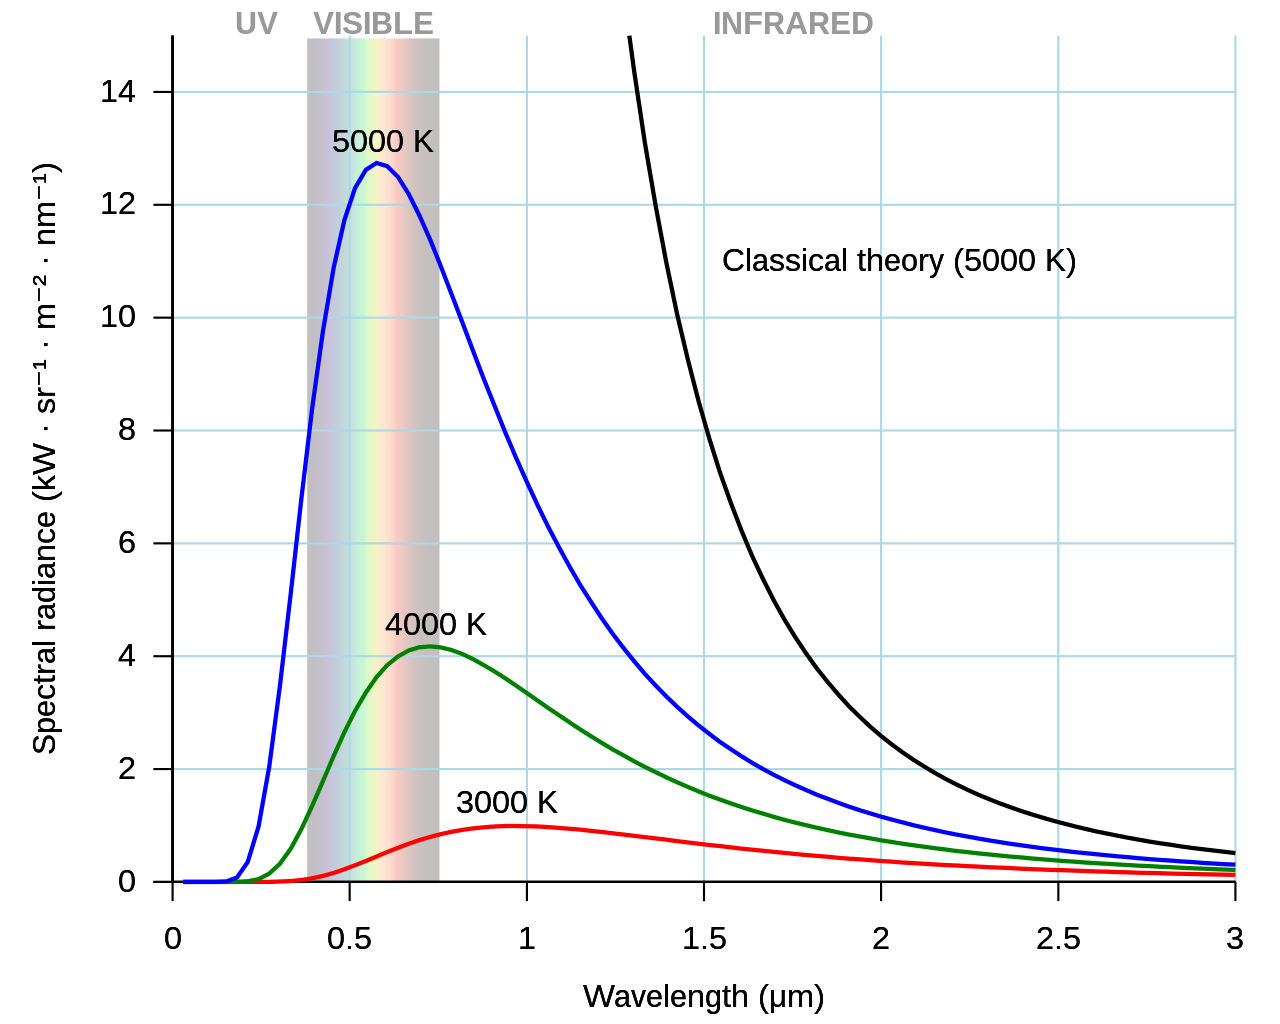
\includegraphics[scale=0.25]{Black_body.svg.png}
\end{center}

By fitting (RP) to experimental data, one finds:
\begin{align*}
h = 6.626076 \ee{-34}\, J\cdot s
\end{align*}
Note that the Planck's constant $h$ is incredibly small, which is the reason why we do not see obvious effects of quantum mechanics in macroscopic systems. Also not that (RP) is well behaved in all wavelengths.\\

Moreover, integrating $R(\lambda,T)$ over all wavelengths we obtain the Stefan-Boltzmann Law:
\begin{align*}
\int_0^{\infty} R(\lambda, T) \, d\lambda = \sigma T^4
\end{align*}
taking the derivative of $R$ and find the maximum yields the Wien's Law. In the limit of $(\frac{hc}{\lambda T})\to 0$, (RP) yields the classical Rayleigh-Jeans results. \\

Up to this point, we showed how the hypothesis of quantization of energy, proposed by Planck, solved the problem of the blackbody radiation. \\


The ultimate blackbody radiation system is the entire universe itself. Hubble discovered the expansion of the universe at the Mt. Wilson Observatory in 1929. The implication of his observation is that in the past, the universe was denser, and hence hotter, than it is today. \\

\subsection{The universe and its expansion}
The early universe was a hot plasma of particles, including photons, and was in thermal equilibrium. The system was too hot to form atoms, at first, opaque to radiation. As the universe expanded, it cooled down, and when cool enough for electron and proton to form hydrogen, we say that the universe became transparent, where the photons traveled freely through the universe ever since, resulting radiation. Since there is nothing to absorb the photons, the cosmic radiation should behave like a blackbody. Theoretical calculations estimated such background radiation in around $1\, mm$ wavelengths, which are the microwaves. \\

In 1965, Penzias and Wilson worked for Bell Labs and were troubled by a persistent noise while attempting to build an antenna to communicate with a satellite, the effective temperature of the noise was $3\,K$. They later came across a calculation by Dicke and Peebles and figured they had discovered the cosmic microwave background (CMB) radiation, for which they received the 1978 Nobel prize for their discovery.\\


Due to the large amount of Hydrogen in the universe, there must have been intense radiation in the early universe to prevent the creation of heavy elements.
The following rapid expansion of the universe lowered the equivalent temperature of the radiation to around a few K. Here the box from the Blackbody model is the entire universe.\\

In fact, high-precision measurements of the CMB sky map of the universe reveal tiny anisotropies. In order to see those anisotropies, we need to subtract foregrounds such as the dipole anisotropy due to the movement of the solar system relative to the reference of the CMB. Detailed mapping of the CMB shows that there are angular anisotropies, at the scale of one part in $10^{-5}$. These anisotropies carry an imprint of physical processes that occurred in the early universe: we can see all the way back to ~300,000 years after the Big Bang. Mather and Smoot won the 2006 Nobel prize for the discovery of CMB spectrum and its anisotropies with the COBE satellite (1993). Since then, new satellites WMAP (2010) and Planck (2014) have measured the CMB in even greater detail. Peebles won the 2019 Nobel prize for his theoretical work.\\
\newpage

\section{The Photoelectric Effect}
In 1887, while Heinrich Hertz studying electromagnetic waves experimentally, he noticed that the metals sometimes emitted a current when light was shone on them, and when the room is dark, this effect sometimes was gone, and he could not explain that fact. In 1900, Philipp Lenard designed an experiment to study this effect, called the photoelectric effect, which is the emission of electrons when electromagnetic radiation, such as light, hits a material. Electrons emitted in this manner are called photoelectrons. There are several phenomenon that cannot be fully explained classically:
\begin{enumerate}
\item The current is proportional to the incoming light intensity, while this one is expected from the classical picture.
\item Maximum kinetic energy of the photoelectron is independent of the intensity of the light, but in classical theory, the kinetic energy of the light should increase with the intensity of the light. 
\item Maximum kinetic energy is proportional to the frequency of the light, no such relation is expected in the classical theory. Energy of a classical wave depends on amplitude, not frequency. 
\item There is a cutoff frequency below which there is no current. This does not make sense in classical theory either.
\item Photoelectrons are emitted almost instantaneously. While in classical theory, it should take approximately 1 second for electron to absorb enough energy from the plane wave to overcome the work function, the amount of energy needed to remove electron from a metal, a few eV.
\end{enumerate}
The big picture of the explanation of  such effect is that electrons are free to move in metal, but it takes energy to liberate them from the metal, the energy is known as the work function $\phi$, photon interacts and transfer its energy to a single electron such that the electron can gain energy to overcome the work function. Einstein, aware of Planck's solution for the blackbody radiation problem, theorized, in 1905, that the photoelectric effect was a result of the electrons absorbing individual quanta of light, or a photon, with energy proportional to the photon frequency. His theory makes a simple prediction, that there should be a universal relationship, for all metals with a given work function $\phi$, between the maximum frequency energy of the photoelectrons and the frequency of the incident light:
\begin{align}
\text{KE}_{\text{max}} = h \nu - \phi
\end{align}

Millikan's oil drop experiments demonstrated that the electric charge was quantized, and measured its value, as well as its mass and the Avogadro number. At the beginning, Millikan did not believe in the existence of photons, and set up an experimental program to disprove Einstein's theory. His results, published a decade later, proved Einstein's theory instead.  His experiments measured Planck's constant within $0.5\%$ of its currently accepted value. Millikan's data for stopping potential verses frequency for the photoelectric effect fall on a straight line with slope given by:
\begin{align*}
\text{slope} = \frac{h}{e}
\end{align*}
as predicted by Einstein a decade before the experiment. Generalizing, we get the following equation for the photoelectric effect:
\begin{align*}
eV_{s} = h\nu - \phi
\end{align*}
where $V_s$ is the stopping voltage. \\


\note In Planck's equation we know that $[h] = [E] / [f] = kg\,m^2 / s$, which is also the unit of angular momentum. We will see later in this text that $\hbar \coloneqq h/2\pi$ is related to the momentum of an object. \\

\subsection{Applications of the photoelectric effect}
Example application of the photoelectric effect is the photomultiplier tube (PMT), which is widely used in experimental physics. \\

PMTs are particularly suitable for applications that require detection of individual photons with high speed, low noise, and high gain. A PMT consists of an entry window coated with with a thin film-like photocathode, a vaccuum tube and a series of electrodes, called dynodes to amplify the signal. When a photon enters the glass and strikes the photo cathode it liberates a photo-electron that is accelerated towards the first dynode. The multiplier part of the detector consists of
a series of electrodes, called dynodes, each held on a large positive potential than the previous one. Photoelectrons released from the photocathode are accelerated by the voltage applied to the focusing electrodes to impinge on the secondary emissive surface of the first dynode where secondary electrons are generated. This process is repeated in all dynodes of the electron multiplier to in this way amplify the signal. PMTs achieve amplification factors of about 106 or more. PMTs
are able to detect single photons with low noise and ultra-fast response.\\

The PMT is very sensitive, able to detects single photon, very fast, very low noise, and has nano-second time-resolution. Like any detector, the PMT also has limitations, such as (1) dark rate from thermionic emissions, (2) affected by the electronic effects, impurities, and cosmic rays, and (3) sensitive to fairly small energy range, that often require combining them with scintillators. \\

The Lux-Zeplin (LZ) detector, which is the current most sensitive detector seeking to discover the hypothesized dark matter particles, uses two arrays of PMTs.\\

Charged Coupled Device (CCD) are $2$-dimensional arrays of tiny pixels, better suited to make images than PMTs, made of semi-conductor material such as silicon. The photoelectric effect takes place in each pixel, and a carefully arranged scheme of electric potential wells serve to collect the charges. Then the charges are transferred across the array by a series of electric signals and the readout occurs — pixel by pixel.  It is a slow detector compared to PMTs.  \\


Boyle and Smith came up with the idea of the CCD while working for Bell Labs in an effort to develop a device that would be attached to traditional telephones to enable video calls. Market research led the company to drop the Picturephone project shortly thereafter. Boyle and Smith won the 2009 Nobel Prize for the invention of the CCD.\\

The advantages of the CCDs for astronomy includes the fact that the CCDs are in small size, lightweight, hence one can easily pack many CCDs on the focal plane of a telescope. The CCDs have high sensitivity, quantum efficiency, even though it is not very fast and require a series of operation to produce the image. The CCDs is linear response, and cover large dynamic range, with low power and low cost as silicon is cheap and mass production is easy. \\

CMOS have faster readout because the readout electronics is attached to each pixel. However, the electronics take space on the chip, reducing light sensitivity. Also, electronic noise is typically higher compared to CCDs. For professional astronomy applications, CCDs are more suitable than CMOS. But commercial digital cameras typically will have CMOS chips.\\



\section{Wave-Particle Duality}
Maxwell's Theory of electromagnetism predicts the wave nature of the electromagnetic radiation. Experimentally, this had been shown in the 19th century, including the properties of interference, diffraction, reflection, and refraction. 

\subsection{Young's double-slit experiment}
In the basic version of this experiment, a coherent light source, such as a laser beam, illuminates a plate pierced by two parallel slits, and the light passing through the slits is observed on a screen behind the plate. Due to the wave nature of the light, the separation between peaks of intensity in the interference pattern on the screen depends on the wavelength $\lambda $ of the light, the separation between slits $d$, and the distance to the screen $D$. For visible light, we can do this with a macroscopic double-slit setup. The distance $y_n$ from the central maximum on the screen to the $n$-th bright fringe on either side of the central maximum is given by the following:
\begin{align*}
y_n = \frac{n\lambda D}{d}
\end{align*}

\subsection{X-rays and Bragg scattering}
Working with cathode ray tube William Rontgen discovered in 1895 that, when electrons hit the glass, a new type of ray originated, and that could pass through materials and be imaged using a fluorescent screen. No diffraction was observed for such ray, hence, called the X-ray. He was then awarded the first Nobel Prize in 1901. The X-ray was then  used in medical and commercial applications.\\

One can see the wave-like effects of the X-rays, whose wavelength is in the nano-meters range. Using a small enough separation between slits, we can see the effect. Separation between atoms in crystalline structure fits the job description. This can be applied in  the study of crystalline structure of materials.\\

If the separation of atom is denoted as $d$, the incoming X-ray of wavelength $\lambda$ makes an angle $\theta$ with the aligned atoms, then we see constructive interference whenever we have:
\begin{align*}
\sin(\theta) = n \frac{\lambda}{2d}
\end{align*}
such condition is known as the Bragg condition. \\

Taken in 1952, the first X-ray picture of DNA was created by Rosalind Francklin, using the X-ray crystallography, and that revealed the helical shape of the DNA molecule. Watson, Crick and Wilkins received the 1962 Nobel Prize in Physiology/Medicine for this discovery.\\

\subsection{Bremsstrahlung}
The fact that an accelerated, or decelerated charge emits radiation is a classical effect in Maxwell's electromagnetism theory. Electromagnetic waves are a perfectly good way for the electrons to get rid of its energy as it slows down. What cannot be explained by classic electromagnetic theory is the observed upper limit on the frequency of the radiation emitted. We can explain that observation if we consider the particle nature of light, though: if the electron loses energy $\Delta K$, we have:
\begin{align*}
hf_{max} = \Delta K
\end{align*}

\subsection{Compton effect}
Until around 1920, the concept of photon was somewhat controversial. Compton did experiments conceptually akin to the photoelectric effect, but using X-rays. He was interested in scattering X-rays off a metal target, and classically we expect the outgoing wave has the same frequency as the incoming wave, though the outgoing wave might have smaller amplitude. However, this was not what Compton observed. In fact, he found that there is a shift of frequency, which can be accounted by treating the scattering as a collision between two particles: an electron at rest, and a photon with energy $hf$.\\


Further evidence for the particle nature of electromagnetic wave is the electron-position pair creation and annihilation. A pair of electron and position can collide to form gamma ray, and a gamma ray can be used to create a pair of electron and positron.\\

\subsection{de Broglie theory on matter waves}
Now consider a generic particle of non-zero mass, according to Einstein, the rest energy of the particle is proportional to the mass, and according to Planck, that rest energy corresponds to a certain frequency, that is the internal quantum clock $f_0$ of the particle. When the particle is moving, one needs to consider the effect of special relativity, the Lorentz factor $\gamma$ represents how much the measurements of time, length, energy, and other physical properties change for an object while it moves, and it depends on $\beta = v/c$. According to Planck and Einstein, we can write the following:
\begin{align*}
hf_0 = m_0c^2
\end{align*}
when the particle moves, according to theory of relativity, energy increases by $1/\sqrt{1-\beta^2}$ where $\beta = v/c$. To be consistent with Planck the frequency must also change $f_0 \to f$, that is, we write:
\begin{align*}
hf = \frac{m_0 c^2}{\sqrt{1-\beta^2}} = \frac{hf_0}{\sqrt{1-\beta^2}}  \qquad \Rightarrow \qquad f_0 = f\sqrt{1-\beta^2}
\end{align*}
However, for moving objects, the time also dilates. So, observing the particle we have to see its internal clock slow down, that is $f_0$ becomes $f_1$:
\begin{align*}
f_1 = f_0 \sqrt{1-\beta^2} = f(1-\beta^2)
\end{align*}
But here is a contradiction, the energy increase when the internal clock slows down. \\

de Broglie's solution to this contradiction is that there are two waves associated to the particle, one is the spatial wave associated with the motion, with frequency $f$, and the other one associated with the internal clock has frequency $f_1$. One can see that in the rest frame, both frequencies are given by $f_1 = f = f_0$, so both waves are always in phase. \\

Assume now the reference frame moves in speed $v$, with the assumptions that at $t=0$, $x=0$, and both waves are in phase. At time $t$, the particle is at position $x=vt = \beta ct$. The spatial wave is assumed to have speed $u$, then at time $t$, the phase of internal clock advanced by $2\pi f_1 t = 2\pi f_1 x/v$, and the phase of spatial wave has advanced by $2\pi f(t-x/u) =2\pi f(x/v- x/u)$, to make the two phases remain in phase, we require $u$ to satisfies:
\begin{align*}
\frac{fx}{v}\left(1- \frac{v}{u}\right) = \frac{f_1 x}{v}\qquad \Rightarrow \qquad f_1 = f\left( 1 - \frac{v}{u}\right)
\end{align*}
comparing with $f_1 = f_0\sqrt{1-\beta^2} = f(1-\beta^2)$, we get:
\begin{align*}
u = \frac{v}{\beta^2} = \frac{c^2}{v}
\end{align*}
The main point of the deviation given by de Broglie's argument is that these two waves, the particle's internal quantum clock, and the spatial wave associated with its motion, remain in phase for all observers at all times. An important
conclusion follows from this result: that is Planck's quantum hypothesis holds for nonzero mass particles too and is consistent with Einstein's special relativity. The following relativistic relations hold:
\begin{align*}
E = hf \qquad \qquad \qquad p = \frac{h}{\lambda}
\end{align*}
and they define the de Broglie wavelength of a generic particle of nonzero mass:
\begin{align*}
\lambda = \frac{h}{p} = \frac{h}{mv}
\end{align*}
that is, waves are not only for photons, waves can be associated to any particle. This idea was crazy for that time, but there was supportive evidence, de Broglie could explain Bohr's postulated atomic radii as standing wave of electrons. However, the wave nature of macroscopic object is hard to be observed. For a moving baseball, the de Broglie wavelength is given by:
\begin{align*}
\lambda = \frac{h}{p} \approx \frac{6.6\ee{-34}\, J\,s}{(0.145\, kg)\, (44\, m/s)} \approx 10^{-34}\, m
\end{align*}
and for smoke particle:
\begin{align*}
\lambda = \frac{h}{p} \approx \frac{6.6\ee{-34}\, J\,s}{(10^{-12}\, kg)\, (0.01\, m/s)} \approx 6.6\ee{-20}\, m
\end{align*}
for comparison, the radius of a proton is $10^{-15}\, m$, hence the wave property effect for macroscopic particles is hard to be detected. But one can still see the wave nature of microscopic particles, such as the electrons. The crystal lattice size is given by $10^{-10}\, m$, suppose we had an electron of de Broglie's wavelength at an order of $10^{-10}\, m$, we write:
\begin{align*}
p = \frac{h}{\lambda} = \frac{6.6\ee{-34}\, J\,s}{10\ee{-10}\, m} = 6.6\ee{-24}\, kg\, m/s^2
\end{align*}
and hence we have:
\begin{align*}
E = \frac{p^2}{2m_e} = \frac{(6.6\ee{-24}\, kg\, m/s^2)^2}{2\, (9.1\ee{-31}\, kg)} = 2.4\ee{-17}\, J = 150\, eV
\end{align*}
and this effect can be detected. In 1927, C. J. Davisson and L. H. Germer first observed the diffraction of electron waves using electrons scattered from a particular nickel crystal. Around the same time, G. P. Thomson showed electron diffraction when the electrons pass through a thin metal foils. Davisson and G. P. Thomson shared the 1937 Nobel prize for their discovery. Since then, diffraction has been seen for neutrons, hydrogen atoms, and alpha particles.\\

In a conventional microscope, details can be resolved only if they are larger than the wavelength of the light, that is around $2000$ times magnification, and at a resolution around $200\, nm$. In electron microscopes, beams of electrons with small wavelength is used to see small objects, up to magnification of around $10,000,000$ times, and resopution at $50\, pm$. For even smaller structures we need even higher energy, hence smaller wavelengths. Of course then the seeing analogy is not correct any more here, but the general relationship still holds. \\

\subsection{The double-slit experiment for particles}
The double-slit experiment is set up by shining a beam passes through an aperture with two slits. The wave-nature of the beam particles allows it to pass through both slits and to create an interference pattern. Depending if one, the other, or both slits are open we call these patterns: $I_1$, $I_2$, $I_{1+2}$. For light, or the electromagnetic waves, the results are as expected from classical physics on the wave properties of the light.\\

If de Broglie's idea about the wave nature of all particles is right, we should observe wave-like behaviors for all particles under a similar double-slit experiment for the particles. Consider reducing the intensity such that only one particle is in the experimental volume. Now we see only individual hits appearing as bursts of energy. Yet waiting long enough we still see a interference pattern build up. Closing one of the slits, interference pattern changes but persists, as a result of diffraction. But when one tries to measure which path the particle takes, the pattern on the screen vanishes.\\

In terms of intensities, intensity measured with both slits open is not equal to the sum of the individual intensities:
\begin{align*}
\begin{cases}
I = I_1 = |h_1|^2 & \text{bottom slit covered}\\
I = I_2 = |h_2|^2 & \text{upper slit covered}\\
I = I_{1+2} = |h_1+h_2|^2 & \text{bottom slit covered}\\
\end{cases}
\end{align*}
where $h_1$ and $h_2$ are the amplitude of particle waves. \\

\newpage

\section{Waves and the Uncertainty Principle}
In general, the wave equation is given by:
\begin{align}
\frac{\partial^2 \phi}{\partial x^2} - \frac{1}{v^2}\frac{\partial^2 \phi}{\partial t^2} = 0
\end{align}
with solution given by:
\begin{align}
\phi = Ae^{ikx - i\omega t}
\end{align} 
which satisfies:
\begin{align*}
k = \frac{2\pi}{\lambda} \qquad\qquad\qquad \omega = 2\pi f
\end{align*}
and (7) describes a traveling wave of amplitude $A$, frequency $f$ and speed $v$, given by:
\begin{align*}
v = \frac{\omega}{k} \qquad\qquad\qquad f = \frac{v}{\lambda} = \frac{v k}{2\pi}
\end{align*}
Considering adding two or more waves of same amplitude and closely-spaced frequencies. The result is a modulated wave that travels with a group velocity:
\begin{align*}
\frac{dx}{dt} = v_{group} = \frac{d\omega}{dk}
\end{align*}
note that the group velocity $d\omega/dk$ is not necessarily the same as the phase velocity $\omega / k$. Information travels at the group velocity. \\

Now the question remained is what is oscillating in a de Broglie wave. Max Born's interpretation is that what oscillates is the probability of measuring the particle, such that the integration over all space is unity:
\begin{align*}
\int_{\text{all space}} |\phi|^2 \, dV = 1
\end{align*}
The probability density is the square of a complex wave function. It gives us the probability of observing a particle in a infinitesimal volume element at a given time $t$. Amplitude-modulated traveling waves gives a probability that is high in some regions and low in others, with the group velocity of the modulations representing the speed of the particle. We cannot measure the complex wave-function itself, but it encodes all possible outcomes in a probabilistic fashion. A measurement collapses the wavefunction, that's the reason why we lose the interference pattern once we attempt to measure the path in the double slit experiment. We also note that any wave $\phi(x,t)$ can be obtained using Fourier Transformation:
\begin{align*}
\phi(x,t) = \int_{-\infty}^\infty A(k) e^{i(kx - \omega_k t)}\, dk
\end{align*}
The coefficients $A(k)$ indicate how much of each harmonic is in the wave. We now have what we need to address the key problem: make localized particles out of waves that are generally spread out in space. If you want to localize a particle in space you need a wave packet with a range of momenta. The group velocity of the packet corresponds to the speed of the particle. The square of the amplitude of the packet's wave function gives the spatial probability density. Conversely, if you restrict the momenta, the wave function will spread out in space. \\

Consider a free non-relativistic particle, with phase velocity $v_\phi$ and group velocity $v_g$:
\begin{align*}
v_{\phi}= \frac{\omega}{k} \qquad\qquad\qquad v_g = \frac{d\omega}{dk}
\end{align*}
For a non-relativistic particle, we write:
\begin{align*}
E = \hbar \omega = \frac{p^2}{2m} = \frac{\hbar^2 k^2}{2m} \qquad\qquad\qquad \text{where }=\frac{2\pi}{\lambda}
\end{align*}
where we can compute the velocities:
\begin{align*}
v_{\phi} = \frac{\omega}{k} = \frac{\hbar k}{2m} \qquad\qquad\qquad v_g = \frac{d\omega}{dk} = \frac{\hbar k}{m}
\end{align*}
the velocity of the original particle is given by:
\begin{align*}
v = \frac{p}{m} = \frac{\hbar k}{m}
\end{align*}
here we see that the group velocity corresponds to the velocity of the particle precisely. We could also show this very similarly in the relativistic case. \\

A square pulse, at time $t$ moving with speed $v$, can be described by the superposition of many waves, or a wave packet:
\begin{align*}
\psi(x,t) = \int_{-\infty}^\infty A(k) e^{-(kx - \omega_k t)}\, dk\qquad\qquad\qquad A(k) = \frac{C}{\pi}e^{i(kx_0 +i \omega_k t)}\frac{1}{k}\sin\left( \frac{k\Delta x}{2}\right)
\end{align*}
where $C$ is the amplitude of the square pulse, and $\Delta x$ is the length of the square pulse. The spatial part of the square pulse wave packet at $t=0$ is given by:
\begin{align*}
\psi(x) = \begin{cases}
 C & |x| \leq \Delta x/2\\
 0 & |x| > \Delta x/2
\end{cases}\qquad\qquad\qquad A(k) = \frac{C}{\pi k}\sin\left( \frac{\Delta xk}{2}\right)
\end{align*}
and combining we have:
\begin{align*}
\psi(x) = \int_{-\infty}^\infty A(k) e^{-kx}\, dk
\end{align*}
The function $A(k)$ contains wavenumbers in an infinite range, but the main contributions come from a window around $k=0$. The size of this window $\Delta k$ can be estimated by asking when the sine function first falls to zero, and the answer is when we have approximately $\Delta x \Delta k \approx 1$. Sample analysis applies when one wants to localize a wave packet in time:
\begin{align*}
f(t) = \int_{-\infty}^{\infty}A(\omega) e^{-i\omega t}\, d\omega
\end{align*}

A pulse, or signal, localized in time is represented by a range of frequencies. The conjugate variables are given by $\Delta \omega \Delta t$, and $\Delta x \Delta k$. One can argue that, we can estimate each term by crudely letting the followings hold:
\begin{align*}
\Delta \omega \Delta t \approx 1 \qquad\qquad\qquad \Delta x \Delta k \approx 1
\end{align*}

The uncertainty relations described above are a general feature of classical waves. Quantum nature come into play when we introduce the relationships:
\begin{align*}
p = \frac{h}{\lambda} = \hbar k \qquad\qquad\qquad E= h\nu = \hbar 
\end{align*}
Then the uncertainty relations become:
\begin{align}
\underbrace{\Delta x \Delta p_x \approx \hbar}_{position-momentum} \qquad\qquad\qquad
\underbrace{\Delta E \Delta t \approx \hbar}_{time-energy}
\end{align}
The Heisenberg uncertainty principle is stated as equation (8), and implies that it is impossible to determine both the position and momentum coordinates, or the energy and time coordinate, of a particle with arbitrary precision. The scale of the uncertainty relations is given by Planck's constant given by (8). Because Planck's constant is very small, as far as the macroscopic world is concerned, the uncertainty principle is often negligible. The formulation of the uncertainty principle is one of the many contributions from Heisenberg to modern physics. He won the 1932 Nobel Prize in Physics ``for the creation of quantum mechanics."\\

\example
Say you received a ticket for speeding by an automated traffic monitoring system. 
If the position of the car is determined to within $10\, m$ by the system, find the uncertainty on your speed.
\begin{align*}
\Delta p = \frac{\hbar}{\Delta x} = \frac{1.054\ee{-34}\, Js}{10\, m} \approx 10\ee{-35}\, kg\, m/s
\end{align*}
Assuming that the car weighs $1000\, kg$, the uncertainty on your speed is about $10\ee{-38}\, m/s$. While the uncertainty introduced by quantum mechanics is negligible for macroscopic objects it becomes sizeable at the Quantum level. For electron in atom $\Delta x \approx 10\ee{-10}\, m$, $\Delta p \approx 10\ee{-24}\, kg$, and $\Delta v\approx 10^6\, m/s$. \\


Consider a particle in a $1$-dimensional box with length $L$. Note that the kinetic energy of the particle is proportional to the momentum squared, the uncertainty in momentum is limited  by the size of the box, $\Delta p \approx \hbar/L$. The average of the square of the momentum can be computed from the standard deviation of the mean:
\begin{align*}
(\Delta p)^2 = (p - \overline{p})^2_{avg} = (p^2 - 2p\overline{p}+\overline{p}^2)_{avg} = \overline{p^2}-\overline{p}^2 = \overline{p^2}
\end{align*}
here we have assumed that the mean momentum is zero. As a result, we have:
\begin{align*}
\overline{K} = \frac{\overline{p^2}}{2m} \geq \frac{\hbar^2}{2mL^2}
\end{align*}
Note that the average kinetic energy of the particle in a box is not zero. This energy that a particle has simply by being confined is called the zero-point energy. For macroscopic objects this is, of course, negligible. But for an electron, this energy is not negligible:
\begin{align*}
\bar{E} = \frac{(\hbar c)^2}{2m_e c^2 L^2}= \frac{(197.3\, eV\, nm)^2}{2(511\ee{3}\, eV) (0.1\, nm)}\approx 3.8\, eV
\end{align*}
Most elementary particles decay in an incredibly short amount of time. Measuring the energy of all it's decay particles allows to measure it's variance $\Delta E$ and determine the lifetime.\\

The Observer Effect is related to the Heisenberg Uncertainty relation and often confused with it. Invoked by Heisenberg (Heisenberg microscope) to provide a physical explanation of the uncertainty principle:
Any act of measuring a system results in a change because some interaction has to occur.
Example includes determining path of electron in the double slit experiment, to see the electron an electron-photon-scattering mechanism has to occur, and hence changes the momentum of the particle. Observer effect is real, but it is not exclusive to quantum mechanics and it not the same as the uncertainty principle. The uncertainty principle is a purely quantum mechanics property due to the wave nature of particles.\\

The uncertainty principle concerns ensembles. When measuring a single particle you will get a definite number for momentum and position, or other conjugate variables. However, if you would measure this particle over and over again, an ensemble of particles, then the measurements will distribute with an uncertainty described by the uncertainty principle.\\





\newpage
\section{The Models of Atoms}
By the end of 19th century, it was generally agreed that matter was made of atoms, but their physical model was unknown. At the time, it was known that:
\begin{enumerate}
\item Atoms are very small, only $0.1\,nm$ in size. Their collective behavior in macroscopic matter is well described by statistical mechanics.
\item Atoms are stable, whatever forces hold them together must be equilibrium.
\item Atoms contain electrons, discovered by J.J. Thomson in the late 1890s. To remain neutral, they must contain some positive charge as well.
\item Atoms can emit and absorb electromagnetic radiation, the spectral lines. Each element has unique spectral fingerprint of frequencies at which it can do this.
\end{enumerate}

Gauss's law from classical electromagnetism implies that the electric field grows linearly with radius inside the atom. Hence electrons are bound by a restorative force, they are harmonic oscillators. Thomson's model proposed that atom consists of positively charged pudding in the middle, and negatively charged plums around the surface of the pudding. But the problem of this model is that no atomic spectral features is included, and no stability for the electrons, that is electrons would radiate energy and quickly decay.\\

Rutherford led a series of experiments to probe the structure of atoms using a beam of alpha particles, the double-ionized helium. He worked with his colleague Geiger and an undergraduate assistant Marsden. They expected the alpha particles to be scattered at small angles. Based on the Thomson model, scattering on gold atom $q = 73\, e$, and alpha particle is doubly-charged He atom, then the maximal force is given by:
\begin{align*}
F_{max} = \frac{1}{4\pi \epsilon_0} \frac{(2e)\cdot (79e)}{(1\ee{-10}\, m)^2} = 3.6\ee{-6}\, N
\end{align*} 
that is the acceleration of the alpha particle is around $5.4\ee{20}\, m/s^2$, so the estimated change in velocity is around $\Delta v = 6750\, m/s$, and the scattering angle is only around $\Delta \theta = 0.01^\circ$. But in fact, a very small number of alpha particles are significantly deflected, and few alpha particles are slightly deflected, and most alpha particles pass straight through the foil. Rutherford then proposed a radical new model for the atom. The positive charge is concentrated on a much smaller region at the center. Deflection angle can be computed using $1/r^2$ force law. The impact parameter for one alpha particle scattering off of one target nucleus at an angle $\theta$ is given by the following:
\begin{align*}
b = \frac{1}{4\pi \epsilon_0} \frac{(ze)(Ze)}{2K_{\alpha}} \cot(\theta/2)
\end{align*}
where $K_{\alpha}$ is the kinetic energy of the incoming alpha particle, $ze$ and $Ze$ are the charges of the alpha particle and the nucleus, respectively. \\

For a beam of particles incident on a foil that is a few hundreds of atoms thick, given a $\theta$, we are interested in what fraction of particles that are scattered at an angle greater than $\theta$. In other words, we want to find what fraction of particles have impact parameters less than $b(\theta)$. It turns out that, the fraction is given by:
\begin{align*}
f_{>\theta} = nb^2 nt
\end{align*}
where $n$ is the number density of atoms per unit volume and $t$ is the thickness of the target. In order to compare with the experimental data, it is useful to convert the expression above into a function of the the scattered angle. This is known as Rutherford's scattering formula:
\begin{align*}
\Delta N = \frac{nt}{4r^2}\left( \frac{zZ}{2K_{\alpha}}\right)^2\left( \frac{e^2}{4\pi \epsilon_0}\right)^2 \frac{1}{\sin^4(\theta/2)}
\end{align*}
for angles between $\theta$ and $\theta + \Delta \theta$. Geiger and Marsden confirmed the predictions made by this formula. Linear dependency on the thickness $t$, linear dependence on the target density $n$, and quadratic dependence on the nuclear charge of the target.
The Nucleus was then discovered.
These investigations were the origin of the modern view of the atom, and gave birth to the field of nuclear physics. \\

Rutherford in 1913 proposed that atom has a compact positive charge in the center akin to a mini solar system. Coulomb forces instead of gravity dominates in such configuration. However, the model has shortcomings:
\begin{enumerate}
\item Why do atoms have the size they do?
Classically, any size orbit is allowed.
Why are atoms of a given substance are all identical? Classically, there are infinitely many possible orbits.
\item Why are atoms stable? Classically, electrons would radiate away all its energy in a fraction of a second, and classically electron would radiate away all of its energy in less than $1\, \mu s$ in a continuous emission spectrum.
\item Why are there discrete features in the atomic spectra? Classically, there is no explanation for this at all. 
\end{enumerate}


Spectral lines had been observed since the 1800s for several elements. For Hydrogen, Johann Balmer derived a series of lines obeying a simple formula in 1885, and Rydberg-Ritz derived an empirical formula that includes Balmer's formula as a special case:
\begin{align*}
\frac{1}{\lambda} = R_{\infty}\left( \frac{1}{n^2} - \frac{1}{m^2}\right)
\end{align*}
where $R_{\infty}$ is a constant, $n$ is the series number, $m$ is the index number, and $\lambda $ is the wavelength of light emitted.\\

Helium was first discovered on the sun by studying light during a solar eclipse in 1868. For some time it was assumed Helium exists only on the Sun, but then it was discovered on Earth about two decades later.\\

Bohr believes that Planck's rule must play a role, and hence we apply dimensional analysis on the $H$ atom. The circular orbit of the electrons is held by Coulomb's force:
\begin{align*}
m\omega^2 r  =\frac{mv^2}{r} = \frac{1}{4\pi \epsilon_0}\frac{e^2}{r^2}
\end{align*}
kinetic energy and orbital frequency are given by:
\begin{align*}
K = \frac{1}{2}mv^2 = \frac{e^2}{8\pi \epsilon_0 r} \qquad\qquad\qquad \omega = \frac{v}{r} = \sqrt{e^2	4\pi \epsilon_0 r^3 m}
\end{align*}
If $K$ is associated with $\omega$ by Planck's formula $\hbar	\omega = K$, we get:
\begin{align*}
r = \frac{16\pi \epsilon_0 \hbar}{mc^2} = 0.2\, nm
\end{align*}
That is, Bohr postulates that atoms can be in certain stationary states without radiating. Atom radiates when making transitions from one state to the other, so called the quantum leap. Change in state via absorption or emission. The frequency of radiation emitted or absorbed is related to Planck s equation: two states with energies $E$ and $E'$, then $hf = E - E'=\Delta E$. Classically $f$ would be related to to angular velocity of the electron. The allowed  states correspond  to  classical  circular  orbits  have  energies  determined  by  the condition that their angular momentum is quantized as an integer multiple of $\hbar$. This is a consequence of the correspondence principle, predictions of quantum and classical theories must agree in the classical regime. Revisiting the hydrogen atom, we have circular orbit held by Coulomb's force:
\begin{align*}
m\omega^2 r  =\frac{mv^2}{r} = \frac{1}{4\pi \epsilon_0}\frac{e^2}{r^2}
\end{align*}
angular momentum $L$ and orbital velocity $v$ are given by:
\begin{align*}
L = mvr \qquad\qquad \qquad v=\frac{e^2}{4\pi \epsilon_0 L}
\end{align*}
using the quantization rule, we obtain discrete orbits:
\begin{align*}
L = mvr = \frac{nh}{2\pi} = n\hbar  \qquad\qquad\qquad \text{for }n \in \N
\end{align*}
and we can rewrite:
\begin{align*}
v_n = \frac{e^2}{4\pi \epsilon_0 n \hbar} \qquad\qquad\qquad r_n = \frac{L_n}{mv_n} = \frac{n\hbar}{mv_n} = n^2 \left( \frac{\hbar}{mc \alpha}\right)
\end{align*}
where we have:
\begin{align*}
\alpha \coloneqq \frac{e^2}{4\pi \hbar \epsilon_0 c} \approx \frac{1}{137}
\end{align*}
The fine-structure constant $\alpha$ was first discovered by Sommerfeld in his study of the fine structure of spectral lines. $\alpha$ is a dimensionless constant that quantifies the strength of the electromagnetic interaction between elementary charged particles. Incredible importance for our existence: if were $\alpha$ to change by $4\%$, stellar fusion would not produce carbon, so that carbon-based life would be impossible. If $\alpha$ were greater than $0.1$, stellar fusion would be impossible, and no place in the universe would be warm enough for life as we know it.\\

Now we can use $r_n$ to calculate characteristic size of atom, for $n=1$, we have:
\begin{align*}
r_1 = \frac{\hbar}{mc\alpha} = 0.0529\, nm
\end{align*}
which is the smallest possible size of an atom. The total energy of an atom, the kinetic energy together with the Coulomb potential, is given by:
\begin{align*}
E = \frac{1}{2}mv_n^2 + V = \frac{1}{2}mv_n^2 - \frac{e^2}{4\pi \epsilon_0 r_n} = -\frac{me^4}{32\pi^2 \epsilon_0^2 \hbar^2}\frac{1}{n^2} = -\frac{1}{2}\frac{m(c\alpha)^2}{n^2} = -\frac{13.6\, eV}{n^2}
\end{align*}
where we get the quantization rule for energy levels of atom, and $13.6\, eV$ is the ionization energy of Hydrogen. The transitions between states $n$ and $m$ result in the following:
\begin{align*}
\nu_{n \to m} = \frac{E_n - E_m}{h} = \frac{mc^2\alpha^2}{2h}\left( \frac{1}{n^2} - \frac{1}{m^2}\right)
\end{align*}
and that explains the Rydberg-Ritz empirical formula:
\begin{align*}
\frac{1}{\lambda} = R_{\infty}\left( \frac{1}{n^2} - \frac{1}{m^2}\right)
\end{align*}
Bohr's idea is that electrons in an atom can only exist in special orbits that obey a quantization condition for the angular momentum.
In terms of the probabilistic interpretation of  the wave function, only  if  an  integral number  of  wavelengths  fit around the orbit will get constructive interference, that is a  nonzero  probability of finding an electron. To fit an integer number of waves around the orbit and using de Broglie's relation between $\lambda$ and momentum, we get the angular momentum quantization:
\begin{align*}
2\pi r = \frac{nh}{p} \qquad \Rightarrow \qquad pr = n\hbar \qquad \Rightarrow \qquad L = n\hbar
\end{align*}


For heavier atoms, however, interactions between multiple electrons complicate matters. If you can remove all but one electron from a heavier atom, the model works well enough, though. Also, the model treats the nucleus as an infinitely massive fixed center. A more accurate treatment, however, should include the reduced mass instead. This will lead to a correction on the value of the constant in the Rydberg-Ritz formula:
\begin{align*}
R(Z,A) = Z^2 \left( 1-\frac{m}{Am_p}R_{\infty}\right)
\end{align*}

\hfill\break\hfill\break
Now we have seen Planck's quanta of energy, de Broglie's matter waves, and Bohr's model for the atom. These are elements of what is now known as the old quantum theory. By the mid-1920s it was clear that, if we were to take the idea of wave nature of particles seriously, we needed a wave equation to describe the dynamics of the particles. The wave function will be the solution of the wave equation. In other words, the wave equation tells how the particle wave function evolves in time and space. In electromagnetism, the wave equation is a consequence of Maxwell's equations. In quantum mechanics, the wave function squared is the probability of making a measurement on the particle. Solution of the wave equation must be normalized. Localized particles are wave packets traveling at the group velocity. We need a linear equation, which enables use of the principle of superposition to make packets 
and makes normalization easy. The wave equation must also satisfies conservation of energy and the de Broglie hypothesis.\\

\newpage
\section{Schrodinger's Equation}
The wave function of photons is implied by the electromagnetic wave equation:
\begin{align}
\left( \frac{\partial^2}{\partial x^2} - \frac{1}{c^2}\frac{\partial^2}{\partial t^2}\right) \psi(x,t) = 0
\end{align}
one solution is a plane wave described by the following:
\begin{align*}
\psi = \psi_0 e^{i(kx - \omega t)} \qquad\qquad \qquad \frac{\omega}{k} = c
\end{align*}
Now we introduce the quantum relations:
\begin{align*}
E = \hbar \omega \qquad\qquad\qquad p=\hbar k
\end{align*}
these allow us to build a solution for the wave equation of photon in terms of the energy and momentum of the particle:
\begin{align*}
\mathcal{E} = \mathcal{E}_0 e^{\frac{i}{\hbar}(px-Et)}
\end{align*}
using this solution in the wave equation (9), we find that:
\begin{align*}
\left( p^2 - \frac{E^2}{c^2}\right) \mathcal{E}(x,t)  =0 \qquad\Rightarrow \qquad p^2c^2 = E^2
\end{align*}
That is the wave equation operator, when applied to a plane wave solution gives the energy-momentum relationship of the particle. We can use this fact to generalize the procedure above to particles with mass greater than zero, relativistic or non-relativistic energy-momentum relation, and particles subject to a potential.
\\

For relativistic particle with mass greater than zero, we use the energy-momentum relation $p^2c^2 + m^2c^4 = E^2$ and postulate a solution of the form:
\begin{align*}
\phi(x,t)= A^{\frac{i}{\hbar}(px-Et)} 
\end{align*}
and wave equation that works here is given by the following:
\begin{align}
\left( \frac{\partial^2}{\partial x^2} - \frac{1}{c^2}\frac{\partial^2}{\partial t^2} - \frac{m^2 c^2}{\hbar^2}\right) \phi(x,t) = 0
\end{align}
Equation (10), known as the Klein-Gordon's equation, is not the equation that we are looking for because it does not work for non-relativistic energy momentum relation, and it also does not take into the account the spin for particles such as the electron.\\

Starting with the non-relativistic equation for a free particle, we again postulate a plane wave solution:
\begin{align*}
E = \frac{p^2}{2m} \qquad\qquad\qquad \psi(x,t) = Ae^{\frac{i}{\hbar}(px-Et)}
\end{align*}
hence we want to find an operator $H$ that satisfies:
\begin{align*}
H\psi = \left( \frac{p^2}{2m}-E\right) \psi = 0
\end{align*}
we can get the $p^2$ factor by differentiating twice with respect to $x$, but to get a single power of $E$, we need to differentiate only once with respect to time, in which case the following equation works:
\begin{align}
\left( \frac{\hbar^2}{2m}\frac{\partial^2}{\partial x^2} + i\hbar \frac{\partial }{\partial t}\right) \psi(x,t) = 0
\end{align}
from this construction, equation (11) reads the Schrodinger's equation:
\begin{align*}
-\frac{\hbar^2}{2m}\frac{\partial^2\psi}{\partial x^2} = i\hbar \frac{\partial \psi}{\partial t}
\end{align*}
If one adds a potential $V(x,t)$, we get the following form:
\begin{align}
-\frac{\hbar^2}{2m}\frac{\partial^2 \psi}{\partial x^2} + V(x,t) \psi = i\hbar \frac{\partial \psi}{\partial t}
\end{align}
Here (12) reads the general form of the Schrodinger's Equation. Note that (12) is linear, we can add two or more solutions and still have a solution. We can multiply a solution by a constant and still have a solution, which makes it easy to satisfy our normalization condition. Energy conservation is built-in in (12). de Broglie relationships are built-in as well. We used these when we replaced $k$ and $\omega$ in our plane wave solutions.
Note the appearance of the imaginary unit in this equation, which means that $\psi$ is necessarily a complex function. This is definitely not your ordinary wave equation.
Note also that the equation above is for a non-relativistic particle. If the particle moves in relativistic speed, the solution is given by the  Dirac equation, which is beyond the scope of this course. Dirac and Schroedinger shared the Nobel prize in 1933 for their discoveries. \\

One can use the separation of variables to solve (12), and for simplicity, here we assume that $V$ depends only on $x$, being independent on time $t$:
\begin{align*}
\psi(x,t) = u(x)T(t) 
\end{align*}
in which case we can write:
\begin{align*}
T\left( -\frac{\hbar^2}{2m}\frac{d^2u}{dx^2} + V u\right) = i\hbar u \frac{dT}{dt}\qquad\Rightarrow\qquad  
\frac{1}{u}\left( -\frac{\hbar^2}{2m}\frac{d^2u}{dx^2} + V u\right) = i\hbar \frac{1}{T} \frac{dT}{dt}\qquad\qquad 
\end{align*}
The LHS is dependent on $x$ only, while the RHS is dependent on $t$ only, hence only way to satisfy both sides of the equation is to have them be a constant $E$. This leads to two equations, one time-dependent equation and the time-independent Schrodinger equation. The solution is then given by the following:
\begin{align*}
\psi(x,t) = u_E(x) e^{-\frac{iEt}{\hbar}}
\end{align*}
where $u_E(x)$ satisfies:
\begin{align*}
-\frac{\hbar}{2m}\frac{d^2u_E}{dx^2} + V u_E = Eu_E
\end{align*}
and $ T(t) = e^{-\frac{iEt}{\hbar}}$ satisfies:
\begin{align*}
i\hbar \frac{dT}{dt} = ET(t)
\end{align*}

Using the Hamiltonian total energy operator definition:
\begin{align*}
\hat{H} = -\frac{\hbar^2}{2m}\frac{\partial^2}{\partial x^2} + V(x)
\end{align*}
we can rewrite the time-independent Schrodinger equation as the following:
\begin{align*}
\hat{H}\psi = E\psi	
\end{align*}

The Hamiltonian acts on the wavefunction and returns the original function multiplied by a constant, $E$. Therefore, the solutions to the time-independent Schroedinger equation are eigenfunctions of the hamiltonian with eigenvalues $E$, which correspond to the stationary states with a definite - quantized - energy. In general, there are many eigenfunctions and eigenvalues. Our job when solving problems is to find them all.\\

\subsection{Free particles}
Here we first consider a free particle, the time-independent Schrodinger's equation reads the following, with $\psi(x)$ denote the wave function of the free particle:
\begin{align*}
-\frac{h^2}{2m}\frac{d^2\psi}{dx^2} = E\psi
\end{align*}
that is, we have:
\begin{align*}
\frac{d^2\psi}{dx^2} + k^2 \psi^2 = 0 \qquad\qquad\text{where }\ \ k^2=\frac{2mE}{\hbar^2} = \frac{p^2}{\hbar^2}
\end{align*}
and hence we have:
\begin{align*}
\psi_p(x,t) = Ae^{\frac{i}{\hbar}(px - E_p t)}+Be^{-\frac{i}{\hbar}(px - E_p t)}
\end{align*}
which describes two plane waves moving left and right. We drop the left-moving one here for say. Note here there is no energy quantization in this case. For definite momentum, there is no localization, hence we need to build a wave packet to localize the particle with momentum between $p_0 - \Delta p/2$ and $p_0 +\Delta p/2$:
\begin{align*}
\psi(x,t) = \int_{-\infty}^\infty A(p) e^{\frac{i}{h}(px-E_p t)}\, dp \qquad\qquad \begin{cases}
A & p_0-\Delta p/2 \leq p \leq p_0 + \Delta p/2\\
0 & \text{otherwise}
\end{cases}
\end{align*}
in which case, at $t=0$, we have:
\begin{align*}
\psi(x,0) = \int_{-\infty}^\infty A(p) e^{ipx/\hbar}\, dp = A\int_{p_0 - \Delta p /2}^{p_0+\Delta p/2} e^{ipx/\hbar}\, dp = 2Ae^{ip_0 x/\hbar}\left( \frac{\hbar}{x}\right) \sin\left( \frac{x\Delta p}{2\hbar}\right)
\end{align*}

\subsection{Infinite quantum well}
Here we will introduce applications of the Schrodinger equation for particles subject of a potential $V(x)$. First we consider infinite square well, a box, that is one dimensional. That is $V(x)$ describes two infinite vertical potential barriers separated by a distance $L$:
\begin{align*}
V(x) = \begin{cases}
0 & 0\leq x \leq L\\
\infty & \text{otherwise}
\end{cases}
\end{align*}
Consider $t=0$, solving the time-independent part of Schrodinger equation, we can write:
\begin{align*}
\psi(x) = Ae^{ikx}+ B e^{-ikx}\qquad\qquad\text{where } \ \ k^2= \frac{2mE}{\hbar^2} = \frac{p^2}{\hbar^2} 
\end{align*}
The probability of finding the particle outside the box is $0$ because the potential is infinite, so we require $\psi(0) = A+B=0$, then we have $A = -B$. Also we require $\psi(L) = 0$, in which case we write the following:
\begin{align*}
\psi(L) = 0 = A(e^{ikL} - e^{-ikL}) = A\sin(kL) 
\end{align*} 
where $kL = n\pi$ for all $n \in \N$, hence we can write:
\begin{align*}
\psi_n(x) = A\sin\left( \frac{n\pi x}{L}\right) \qquad \text{normalizing we get}\qquad \psi_n(x) = \sqrt{\frac{2}{L}}\sin\left( \frac{n\pi x}{L}\right)
\end{align*}
and here the energy is quantized:
\begin{align*}
E_n = \frac{\hbar^2 k_n^2}{2m} = \frac{\hbar^2 \pi^2 n^2}{2mL^2}
\end{align*}
Note that we now have discrete energy levels. This is a consequence of the boundary conditions. Free particle is the case where $L$ tends to infinity.
Each energy level, or eigenvalue, corresponds to a solution, or an eigenfunction. \\


Consider a $2$-dimensional symmetric infinite square well characterized by $V(x,y)$, in which case the time-independent Schrodinger equation reads the following:
\begin{align*}
-\frac{\hbar^2}{2m}\left( \frac{\partial^2}{\partial x^2} + \frac{\partial^2}{\partial y^2}\right) \psi(x,y) + V(x,y)\psi(x,y) = E\psi(x,y)
\end{align*}
using the method of separation of variable, we again obtain the followings, with two quantum numbers $n$ and $m$:
\begin{align*}
\psi_{nm}(x,y) = \frac{2}{L}\sin\left( \frac{n\pi x}{L}\right) \sin\left( \frac{m\pi y}{L}\right)\qquad\qquad E_{nm} = \frac{\hbar^2\pi^2}{2mL}(n^2+m^2)
\end{align*}
Note that there is now a degeneracy, that is more than one quantum state, characterized by a combination of quantum numbers, can be associated with the same energy. The system can transition between two degenerate states without consuming energy, expect to see implications for statistical behavior. It is possible to lift the degeneracy by making the lengths in $x$ and $y$ different, that is by breaking the symmetry of the system.\\

\subsection{Finite quantum well}
Now consider a $1$-dimensional finite square well. In region II, the potential is $0$, and in region I and III, the potential is $V_0$:
\begin{center}
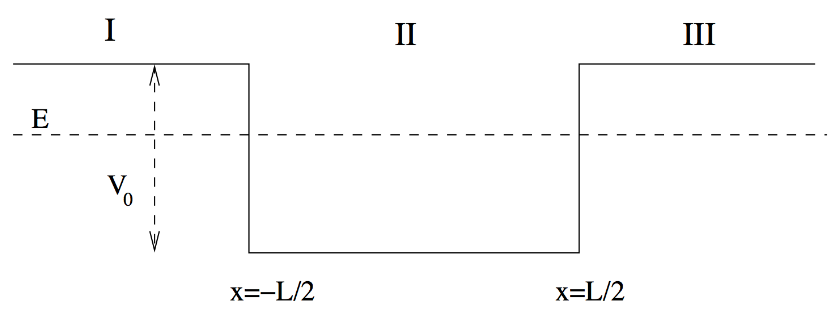
\includegraphics[scale=0.39]{quantumWelll.png}
\end{center}

If the particle's total energy is greater than the well barrier, the particle is free and hence the wave solution is free particle solution:
\begin{align*}
\psi(x,t) = \int_{-\infty}^\infty A(p) e^{\frac{i}{h}(px-E_p t)}\, dp \qquad\qquad \begin{cases}
A & p_0-\Delta p/2 \leq p \leq p_0 + \Delta p/2\\
0 & \text{otherwise}
\end{cases}
\end{align*}
If the total energy is below the barrier. In region I and III, we have the followings:
\begin{align*}
-\frac{\hbar^2}{2m}\frac{d^2\psi}{dx^2}+V_0 \psi = E\psi \qquad \Rightarrow \begin{cases}
\psi_I(x) = Ce^{\alpha x} & x<-L/2\\
\psi_{III}(x) = De^{-\alpha x} & x>L/2
\end{cases}
\end{align*}
where we write:
\begin{align*}
\alpha^2 = \frac{2m}{\hbar^2}(V_0 - E)>0
\end{align*}
In region II, the situation is similar to the infinite square well, except for the boundary conditions. The wave function in this region cannot fall to zero at the edges of the well, it must connect smoothly to solutions in regions I and III so that the total wave function can be normalized in the entire infinite range of x values. Using the boundary conditions to find the constants, we obtain the relation:
\begin{align*}
\tan(kL/2) = \tan\left( \frac{L}{2}\sqrt{\frac{2mE}{\hbar^2}}\right)
\end{align*}
which can be satisfied only for a finite number of values of $E$, that means that we have a finite number of bound states in this system. That is different from the infinite wall. And we can also see that there is non-zero probability that the particle will penetrate the barrier, classically, that is not expected.\\

\newpage
\section{Quantum Harmonic Oscillator}
The simple harmonic oscillator is one of the most important models in physics. Any system with a minimum energy can be approximated via a quadratic potential, such as diatomic molecules, lattice vibrations in materials, and quantum fields in particle physics.\\

In classical physics, for simple harmonic system, the total energy of the system can be written as the following:
\begin{align*}
E = \frac{1}{2}mv^2 + \frac{1}{2}kx^2 = \frac{p^2}{2m}+\frac{1}{2}m\omega^2 x^2
\end{align*}
Here we consider the quantum operators under canonical transformations:
\begin{align*}
\hat{P} = -i\hbar \frac{d}{dx} \qquad\qquad\qquad \hat{X} = x
\end{align*}
From time independent Schrodinger equation, we can write the following:
\begin{align*}
\frac{1}{2m}\left( \left( \frac{\hbar}{i}\frac{d}{dx}\right)^2 + (m\omega \hat{X})^2 \right) \psi = \frac{1}{2m}\left( \hat{P}^2 + (m\omega \hat{X})^2 \right)\psi = E\psi
\end{align*}

On the other hand, the time independent Schrodinger equation reads:
\begin{align*}
\hat{H}\psi = E \psi
\end{align*}
Here we consider the terms given by the followings:
\begin{align*}
a = \frac{1}{\sqrt{2m}}\left( \hat{P} - im \omega \hat{X}\right) \qquad\qquad\qquad a^\dagger = \frac{1}{\sqrt{
2m}}\left( \hat{P} + im \omega \hat{X}\right)
\end{align*}
We expect $aa^\dagger = a^{\dagger}a = \bar{H}$ if $a$ commutes with $a^{\dagger}$. Here we call $a$ as the annihilation operator and $a^{\dagger}$ as the creation operator. One can compute that we get the followings:
\begin{align*}
aa^{\dagger} = \frac{1}{2m}\left( \hat{P}^2 + (m\omega \hat{X})^2 \right) + \frac{1}{2}\hbar \omega \qquad\qquad\qquad a^{\dagger}a = \frac{1}{2m}\left( \hat{P}^2 + (m\omega \hat{X})^2 \right) - \frac{1}{2}\hbar
\end{align*}
and therefore, for the $aa^\dagger$ and $a^\dagger a$, we can write the Hamiltonian of the system in two ways, given by the followings:
\begin{align*}
\hat{H} = aa^{\dagger} - \frac{1}{2}\hbar \omega \qquad\qquad\qquad \hat{H} = a^{\dagger}a + \frac{1}{2}\hbar \omega
\end{align*}
and the commutator of $a$ and $a^{\dagger}$ is defined to be the following:
\begin{align*}
\left[ a, a^{\dagger}\right] = aa^{\dagger} - a^{\dagger}a = \hbar \omega
\end{align*}
in which case we say $a$ and $a^{\dagger}$ do not commute, and here $a$, $a^{\dagger}$ are called the ladder operator. In particular, they satisfy the following properties, with $\psi$ being an eigenfunction of $\hat{H}$ corresponds to eigenvalue $E$:
\begin{align*}
\hat{H}\left(a^{\dagger}\psi\right) &= \left( a^{\dagger}a + \frac{1}{2}\hbar\omega \right) a^{\dagger}\psi \\
&= a^\dagger\left( aa^{\dagger}+ \frac{1}{2}\hbar \omega \right) \psi\\
&=a^\dagger \left( (\hbar \omega + a^{\dagger}a) + \frac{1}{2}\hbar \omega \right) \psi\\
&= a^{\dagger}\left( \hbar \omega \psi + \left( a^{\dagger}a + \frac{1}{2}\hbar \omega \right) \psi\right) \\
&= a^{\dagger}\left( \hbar \omega \psi + E \psi\right)\\
&= (E+ \hbar \omega ) \left( a^{\dagger} \psi\right)
\end{align*}
similarly, we can obtain the following result for $a$:
\begin{align*}
\hat{H}(a\psi) = (E-\hbar \omega) (a\psi)
\end{align*}
that is, we see that if $\psi$ is a solution of the Schrodinger equation, then $a^\dagger \psi$ and $a\psi$ are also solution to the Schrodinger equation. That is, we can use the $a^{\dagger}$ and $a$ operators to obtain more solutions of the Hamiltonian, with the properties that $a^{\dagger}\psi$ corresponds to an eigenstate with energy unit $\hbar \omega$ greater than that of $\psi$, and $a\psi$ corresponds to an eigenstate with energy unit $\hbar \omega$ less than that of $\psi$. The operators can be said to have created or annihilated one quantum energy equal to $\hbar \omega$ and can be used to successively to generate any other states. One can also define the number operator:
\begin{align*}
\hat{N} = \frac{a^\dagger a}{\hbar \omega}
\end{align*}
the number of the current energy level is given by applying the number operator on the state:
\begin{align*}
\hat{H}\psi = \left(a^\dagger a + \frac{1}{2}\hbar \omega \right) \psi = \hbar \omega \left( \hat{N} + \frac{1}{2}\right) \psi = \left( n + \frac{1}{2}\right) \hbar \omega \psi \coloneqq E_n \psi
\end{align*}
Note that ladder operators are not measurable, we can use them to obtain all solutions of the harmonic oscillator and its energy levels. In fact, the solutions and energy levels of the quantum harmonic oscillator is given by the followings:
\begin{align*}
\psi_n = A_n \left( a^\dagger\right)^n e^{-\frac{m\omega}{2\hbar}x^2} \qquad\qquad\qquad E_n =\left( n+\frac{1}{2}\right) \hbar \omega = \left( n+\frac{1}{2}\right) hf
\end{align*}
where, as we have defined previously:
\begin{align*}
a^\dagger = \frac{1}{\sqrt{2m}}\left( \frac{\hbar}{i}\frac{d}{dx}+im \omega x\right)
\end{align*}
The solutions $\psi_n$ turn out to be of the following form:
\begin{align*}
\psi_n  = A_n H_n e^{-\frac{m\omega}{2\hbar}x^2}
\end{align*}
where $H_n$ is the Hermite polynomial of degree $n$:
\begin{align*}
H_0 = 1 \qquad \qquad H_1 = 2x \qquad\qquad H_2 = 4x^2 - 2 \qquad\qquad H_3 = 8x^3 - 12x \qquad \qquad \cdots
\end{align*}
Notice that, the energy of the minimal state $\psi_0$ is not zero, but $\frac{1}{2}\hbar \omega$. At the minimal state, the largest probability to find oscillator is at the position $x=0$, smallest probability at the turning points, and there is finite probability to be outside the potential $V(x)$.  Classically, the particle would have negative kinetic energy if it were to be found beyond the oscillator's turning point, which is impossible in the classical theory, we would like to reconcile this with the results we have. In the quantum case, the wave function falls off exponentially beyond the turning point:
\begin{align*}
\psi_n \propto e^{-a x^2}
\end{align*}
So its range in the forbidden zone is limited to around $\Delta  x$ from the classical turning point:
\begin{align*}
\Delta x = \frac{1}{\sqrt{a}} = \sqrt{\frac{2\hbar}{m \omega}}
\end{align*}
Finding the particle beyond this point, then corresponds to localizing it within roughly the distance $\Delta x$. By uncertainty principle, this implies an uncertainty in momentum given by:
\begin{align*}
\Delta p = \frac{\hbar}{\Delta x} =\sqrt{\frac{m\omega \hbar}{2}}
\end{align*}
this leads to an uncertainty in the kinetic energy:
\begin{align*}
\Delta K = \frac{(\Delta p)^2}{2m} = \frac{1}{4}\hbar \omega  \approx E_0
\end{align*}
so the uncertainty in the energy is on the same order as the total energy we thought the particle might have, and this uncertainty is just enough energy to prevent us from observing a negative kinetic energy. \\

\newpage
\section{Tunneling Phenomenon}
A free particle is the one that is not subject to any force. In terms of the potential, that means that the potential is constant. Here we first restore the time-dependence to our solutions. Via Schrodinger's equation, generalizing the free particle equation to include a non-zero constant potential $V_0$, we can write the following:
\begin{align*}
-\frac{\hbar^2}{2m} \frac{d^2 \psi}{dx^2} + V_0 \psi = E\psi \qquad \Rightarrow \qquad \frac{d^2 \psi}{dx^2} + \frac{2m(E- V_0)}{\hbar^2} \psi = 0
\end{align*}
We first define:
\begin{align*}
k = \frac{\sqrt{2m (E-V_0)}}{\hbar} \qquad\qquad\qquad \alpha = \frac{\sqrt{2m(V_0 - E)}}{\hbar}
\end{align*}
In the case where $E>V_0$, we obtain the following time-independent solution:
\begin{align}
\psi(x) = Ae^{ikx} + Be^{-ikx}
\end{align}
where we see that (13) is an oscillatory wave function. \\
In the case where $E<V_0$, we have the following solution:
\begin{align}
\psi(x) = Ae^{\alpha x} + Be^{-\alpha x}
\end{align}
where we see that (14) is an exponential function, and we observe that (14) diverges for $x$ approaching $\pm \infty$. So if $V_0$ exists everywhere, $\psi$ cannot be normalized, in which case we must set $A = B = 0$, that is the particle cannot permanently exist in an energetically forbidden state. \\

In either case, the time-dependent solution is given by appending a factor of $e^{-iEt/\hbar}$, we let $\omega \coloneqq E/\hbar$, then the time-dependent solution for $E>V_0$ is given by the following:
\begin{align*}
\psi(x,t) = \psi(x) \cdot e^{-i \omega t}
\end{align*}

\subsection{The potential step}
Here we will consider what happens when the potential is almost constant, that it is flat everywhere except at one or two points where it undergoes an abrupt step or drop.\\

Now we consider a beam of particles from the right, which has potential $0$, incident on the potential step $V_0$ at position $x=0$. \\

For the case $E>V_0$, we represent the incoming light as:
\begin{align*}
\psi_{\text{inc}}  = Ae^{i(kx - \omega t)} \qquad\qquad x<0 \tag{$E>V_0$}
\end{align*}
where $k = \sqrt{2mE}/\hbar$. Since we have $E>V_0$, we will get a free particle solution on the $x>0$ region:
\begin{align*}
\psi_{\text{trans}} = Ce^{i(k'x -\omega t)} \qquad\qquad x>0 \tag{$E>V_0$}
\end{align*}
where $k' = \sqrt{2m(E-V_0}/\hbar$. there is no left-moving term in the region $x>0$ as we do not expect the transmitted particles to turn around and move backwards. While in the $x<0$ region, we also have the reflected solution:
\begin{align*}
\psi_{\text{refl}} = Be^{i(kx + \omega t)} \qquad\qquad x<0 \tag{$E>V_0$}
\end{align*}
combining, in the $x<0$ region, we write:
\begin{align*}
\psi = \psi_{\text{inc}} + \psi_{\text{refl}} =  Ae^{i(kx - \omega t)} + Be^{-i (kx + \omega t)}  \qquad \qquad x<0 \tag{$E>V_0$}
\end{align*}

Per boundary condition, we requires $\psi$ and $\partial\psi/\partial x$ to be continuous at $x=0$, that is, we require the followings hold:
\begin{align*}
A + B = C \qquad\qquad k(A-B) = k'C \tag{$E>V_0$}
\end{align*}
If one has been thinking of this problem as a traditional particle, one may find this result counterintuitive. A traditional particle would simply go on to the other side of the barrier if the energy is high enough, and there will be no reflection. However, thinking instead of a wave - a beam of light moving from one medium to another - there will be a reflected wave even for high energies. Now we can calculate the fraction of the incident wave that is being transmitted and reflected. Note that the square of the wave function gives the probability, therefore, we can write the reflection coefficient as the following:
\begin{align*}
R = \frac{|B|^2}{|A|^2} = \left(\frac{k-k'}{k+k'} \right)^2  \tag{$E>V_0$}
\end{align*}
and the transmission coefficient as the following:
\begin{align*}
T = 1-R = \frac{4kk'}{(k+k')^2}\tag{$E>V_0$}
\end{align*}\\

Now for the case where $E<V_0$, with similar argument, we get exponential wave function in the region $x>0$, and hence the following solution:
\begin{align*}
\psi = \psi_{\text{inc}} + \psi_{\text{refl}} =  Ae^{i(kx - \omega t)} + Be^{-i (kx + \omega t)} \qquad\qquad x<&0 \\
\psi = \psi_{\text{trans}} = Ce^{-\alpha x - \omega t} \qquad\qquad x>&0 \tag{$E<V_0$}
\end{align*}
where $\alpha = \sqrt{2m(V_0-E)}/\hbar$. The continuity at boundary requires:
\begin{align*}
A+B = C \qquad\qquad ik(A-B) = \alpha C  \tag{$E<V_0$}
\end{align*}
So there is a nonzero probability that the particle penetrates a short distance into the wall. Here we suppose further that the barrier at $x=0$ in fact has finite width $a$, that is the barrier of potential $V_0$ is positioned in the range from $x=0$ to $x=a$. In the region to the right of the barrier, that is the region $x>a$, the potential is back to $0$. Suppose the incoming wave in the region $x<0$ has energy $E<V_0$. Classically we expect only a reflected wave, but in this problem, one can show that there is a nonzero transmitted wave in to the region $x>a$ with transmission coefficient:
\begin{align*}
T \approx 16 \frac{E}{V_0} \left( 1 - \frac{E}{V_0}\right) e^{-2\alpha a} \tag{$E<V_0$}
\end{align*}
in the limit where $\alpha a >>1$. Details of the pre-factor term in $T$ depends on the shape of the potential, but the exponential term is common to all tunneling problems. \\

\subsection{Examples of tunneling}
The probability of tunneling through a wall is extremely small, here using the parameters consistent as we discussed above, assuming that $a$ is a few centimeters, $\alpha \approx \sqrt{2m V/\hbar}$ where $m$ is around a kilogram, and $V$ is around $1 \, J$. The transmission coefficient is given by around:
\begin{align*}
T \approx e^{-10^{34}}
\end{align*}
Do not try to tunnel through a wall at home.\\

For tunneling microscope, the probability density of a tunneling particle is exponentially dependent on the width of the barrier it is tunneling through. A ultra-fine atom sized tip moved at Angstrom precision is able to measure the current when electrons tunnel through the gap. That is the principle of the scanning tunneling microscope.\\

\newpage
\section{The Hydrogen Atom}
The Hydrogen atom is made of a nucleus, usually a proton, with an electron orbiting the nucleus. They constitute around $72\%$ of the baryonic matter in the universe, so, by understanding it well we are making substantial progress towards an understanding of nature. The Hydrogen atom illustrates many important general features of quantum mechanics, such as the angular momentum, that can later be applied to other systems such as the multi-electron atoms and molecules. It is simple enough that the Schrodinger equation can be solved exactly for electrons in hydrogen atom.\\

We consider here the electron orbiting the proton under potential $V$, and we denote the mass of electron as $m_e$. Note here this analysis can be applied to many other systems which has potential in a form similar to the Coulomb potential that the electron in our system is subject to. The time independent $3$-dimensional Schrodinger equation reads:
\begin{align*}
-\frac{\hbar^2}{2m_e}\left( \frac{\pd^2}{\pd x^2} + \frac{\pd^2}{\pd y^2} + \frac{\pd^2}{\pd z^2}\right) \psi + V(x,y,z)\psi = E\psi
\end{align*}
For Hydrogen atom, $V$ is given by the Coulomb potential:
\begin{align*}
V(r) = -\frac{e^2}{4\pi \epsilon_0 r}
\end{align*}
here we will employ the spherical coordinate instead. Combining, the Schrodinger equation reads the following:
\begin{align*}
-\frac{\hbar^2}{2m_e}\left( \frac{\partial^2}{\partial r^2}+ \frac{2}{r}\frac{\pd}{\pd r}+ \frac{1}{r^2\sin(\theta)}\frac{\pd}{\pd \theta}\left( \sin(\theta) \frac{\pd}{\pd \theta}\right)+ \frac{1}{r^2\sin^2(\theta)}\frac{\pd^2}{\pd \phi^2}\right) \psi + V(r) \psi = E\psi
\end{align*}
We look for solutions that are separable into radial component and an angular component, as given by the following:
\begin{align*}
\psi(r,\theta, \phi) = R(r) Y(\theta, \phi)
\end{align*}
Suppose the two equations after separation equal to a constant $l(l+1)$. We will see later that $l$ is the angular momentum quantum number, a non-negative integer. Here we can write the following:
\begin{align}
-\frac{\hbar^2}{2m_e}\left( \frac{d^2R}{dr^2}+\frac{2}{r}\frac{dR}{dr} - l(l+1) \frac{R}{r^2}\right) + V R = ER
\end{align}
\begin{align}
\left( \frac{\pd^2}{\pd \theta^2}+ \cot(\theta) \frac{\pd}{\pd \theta}+ \frac{1}{\sin^2(\theta)}\frac{\pd^2}{\pd \phi^2}\right) Y = -(l+1) Y
\end{align}
Here (16) is the equation for angular wave function. For fixed value of $l$, note that the term $-l(l+1)/r^2$ in (15) acts like a potential term but with opposite sign, which is called the centrifugal barrier. This makes sense because large angular momentum orbits are further from the center. We are interested in bound-state solutions, that implies discrete values of $E$:
\begin{align*}
E = -\frac{m_e}{2}\left( \frac{e^2}{4\pi \epsilon_0 \hbar}\right)^2 \frac{1}{(n_r+l+1)^2} \qquad \Rightarrow \qquad E_n = -\frac{m_ee^4}{32\pi^2 \epsilon_0^2 \hbar^2}\frac{1}{n^2} \approx -\frac{13.6\, eV}{n^2}
\end{align*}
where the principal quantum number is defined as:
\begin{align*}
n = n_r + l + 1 \in \N
\end{align*}
\note The principle quantum number is all we need to determine the energy of the system, in this case, the electron. We see directly here $E$ is quantized. Also note that difference combinations of $n_r$ and $l$ give the same energy level $n$, resulting in degeneracy. \\ 

The solution for (15) takes a form similar to the harmonic oscillator:
\begin{align*}
R_{nl}(r) = C\left( \frac{l}{na_0}\right)^{3/2}\left( \frac{r}{a_0}\right)^l \cdot p_{n-l-1}\cdot e^{-\frac{r}{na_0}}
\end{align*}
where $p_{n-l-1}$ is a polynomial in $r/a_0$ of degree $n-l-1$, and $a_0$ is the Bohr radius:
\begin{align*}
a_0 = \frac{4\pi \epsilon_0 \hbar^2}{m_e e^2} \approx 0.0529\, m
\end{align*}
Note here we must have $n-l\geq 1$. Hence the choice of $l$ is given by $0 \leq l < n$. \\

For angular momentum in classical physics:
\begin{align*}
\vec{L} = \vec{r}\times \vec{p} = (yp_z - zp_y,\ zp_x - xp_z, xp_y - yp_z)
\end{align*}
using the canonical transformations, we get:
\begin{align*}
\hat{L} = \left( -i\hbar \left( y \frac{\pd}{\pd z} - z \frac{\pd}{\pd y}\right), \ -i\hbar \left( z \frac{\pd}{\pd x}-x\frac{\pd}{\pd z}\right), \ -i\hbar\left( x \frac{\pd}{\pd y} - y \frac{\pd}{\pd z}\right) \right)
\end{align*}
Another interesting quantity is the squared of the angular momentum:
\begin{align*}
\hat{L}^2 = \hat{L}_x^2 + \hat{L}_y^2 + \hat{L}_z^2
\end{align*}
and in spherical coordinates, we write:
\begin{align*}
\hat{L}^2 = -\hbar^2 \left( \frac{\pd^2}{\pd \theta^2} + \cot(\theta) \frac{\pd}{\pd \theta}+ \frac{1}{\sin^2(\theta)}\frac{\pd^2}{\pd \phi^2}\right)
\end{align*}
Hence now we have the following according to (16):
\begin{align*}
\hat{L}^2 Y (\theta,\phi) = \hbar^2l(l+1) Y(\theta, \phi)
\end{align*}
and we see immediately that the spherical harmonics $Y(\theta, \phi)$ are eigenfunctions to $\hat{L}^2$. From here, we know that the angular momentum of the system is given by:
\begin{align*}
L = \hbar\sqrt{ l(l+1)}
\end{align*}
and hence we now see why $l$ is called the angular momentum quantum number.\\

Note that the spherical harmonics given by the following form a complete set of basis function on the unit sphere, and it also separate in a $\phi$ and $\theta$ dependent part:
\begin{align*}
Y_{lm}(\theta, \phi) = \epsilon\sqrt{\frac{2l+1}{4\pi}\frac{(l-|m|)!}{(l+|m|)!} }e^{im \phi}p_{lm}(\cos(\theta)) = P_{lm}(\theta)\Phi_m(\phi)
\end{align*}
where $p_{lm}$ is a function of $\cos(\theta)$. This allows us to find the eigenvalues and eigenfunction of $\hat{L}^2$, and $m$ runs from $-l$ to $l$ is called the magnetic quantum number.  \\


Moreover, the $z$-component momentum operator $\hat{L}_z=-i\hbar (\pd/\pd\phi)$ is especially simple. It is not hard to obtain the eigenfucntion for the $\hat{L}_z$ operator in the following form:
\begin{align*}
\Phi_m(\phi) = e^{im \phi}\qquad\text{for } m \in \Z
\end{align*}
Here we require $z$ to be an integer because the function $\phi$ needs to have the same value it started with when the electron orbits around one circle. Moreover, one can verify that $m\hbar$ is the corresponding eigenvalue for $\Phi$, that is:
\begin{align*}
\hat{L}_z \Phi_m = m\hbar \Phi_m
\end{align*}
concluding we know that $m\hbar$ is the quantized $z$-component of the angular momentum. \\

Putting together, the general solution is given of the form:
\begin{align*}
\psi(r,\theta, \phi) = R_{nl}(r) Y_{lm}(\theta, \phi) = R_{nl}(r) P_{lm}(\theta)\Phi_m(\phi)
\end{align*}

The probability to find the particle in a volume element, that is the Cartesian product of radial shell and the solid angle, is given by the following:
\begin{align*}
|\psi|^2 r^2 \sin(\theta)\,dr\, d\theta\, d\phi
\end{align*}
where the total wave function is the product of a radial component and an angular component, hence we write:
\begin{align*}
|\psi|^2 r^2 \sin(\theta)\,dr\, d\theta\, d\phi = |R|^2r^2 \, dr \, |Y|^2\sin(\theta)\, d\theta\, d\phi
\end{align*}
Note that the radial and angular components must be normalized separately:
\begin{align*}
\int_0^\infty |R|^2 r^2 \, dr = 1 \qquad\qquad \int_0^{2\pi} \int_0^{\pi} |Y|^2\, \sin(\theta)\, d\theta d\,\phi= 1
\end{align*}
Looking at the energy eigenvalues, we see many ways to get the same value of $n$ from combinations of $n_r$ and $l$. Moreover, once we consider the angular equation, we see that for a given $l$, there are $(2l+1)$ solutions labeled with the magnetic quantum number, $m$, which can take integer values between $-l$ and $+l$.  Therefore, the number of degenerate states for a given energy level goes up with the square of the principal quantum number $n$. In conclusion, one should note the followings:
\begin{enumerate}
\item The principle quantum number $n$ determines the energy of the system:
\begin{align*}
E=-\frac{m_ee^4}{32\pi^2 \epsilon_0^2 \hbar^2}\frac{1}{n^2} \approx -\frac{13.6\, eV}{n^2}
\end{align*}
\item The angular momentum quantum number $l$ determines the angular momentum of the system: 
\begin{align*}
L = \hbar\sqrt{l(l+1)}
\end{align*}
\item The magnetic quantum number $m$ is the projection of $L$ on the $z$-axis:
\begin{align*}
L_z = m\hbar
\end{align*}
\end{enumerate}
\remark The magnetic quantum number is sometimes called the magnetic moment quantum number. The reason is discussed in the next section.

\newpage
From electromagnetism, the magnetic moment is current times area. If the electron is at an orbit of radius $r$ and orbital frequency $f$, we have $I = qf$ and $L=m_evr$, therefore,
\begin{align*}
\mu = IA= q \left( \frac{v}{2\pi r}\right) \pi r^2 = \frac{1}{2}qvr = \frac{q}{2}\left( \frac{L}{m_e}\right) = -\frac{eL}{2m_e}
\end{align*}
if we write $L = \hbar \sqrt{l(l+1)}$, we get:
\begin{align*}
\mu = -\frac{e\hbar}{2m_e}\sqrt{l(l+1)}
\end{align*}
In specifically, the $z$-component of $\mu$ reads the following:
\begin{align*}
\mu_z = -\frac{eL_z}{2m_e} = -\frac{e\hbar}{2m_e}m \coloneqq -m \mu_B
\end{align*}
where $m$ is the magnetic quantum number, and $\mu_B$ is called the Bohr magneton. From electromagnetism, the energy of a dipole in a magnetic field $\vec{B}$ is given by the dot product of $\vec{B}$ and $\vec{\mu}$, and we can define our $z$-axis such that it aligns with the direction of $\vec{B}$, in which case we have the following:
\begin{align*}
U = -\mu_z B = (\mu_B)m
\end{align*}
Here we note that $m$ is related the direction of the angular momentum vector. It only affects the electron energy when it is in a magnetic field. It determines the energy shift of an atomic orbital due to an external magnetic field, so called the Zeeman effect. \\

\note The quantum number $m$ does not directly affect the energy of the electron when there is no magnetic field presented. 

\newpage
\subsection{The spin and the Stern-Gerlach experiment}
If a beam of atoms is sent through a non-uniform $\vec{B}$ field and collected on a screen at the other end of the tunnel, the dipoles will feel a force depending on how they are oriented with respect to $\vec{B}$. The Stern-Gerlach experiment showed that the the beam of silver atoms, which have $L = 0$, was split into two on the screen. However, in the case $L=0$, we expect to see no split for the beam because we have $L=m=0$ in such case and hence magnetic moment of $0$. Goudsmit and Uhlenbeck's solution to this phenomenon was adding another quantum number. The new quantum number is called the spin, denoted as $s$, and its projection on the $z$-axis is denoted as $m_s$. Spin $s$ is a multiple of half-integers value and is associated with the intrinsic angular momentum of the particle. In particular, the spin of the electron is given by the following:
\begin{align*}
S= \hbar \sqrt{\frac{1}{2}\left( \frac{1}{2}+1\right)}
\end{align*}
There is no classical equivalent for the spin. If one tries to interpret it as a classical spinning sphere, one will get into trouble. \footnote{Goudsmit and Uhlenbeck joined the faculty at U-M in 1927 and were members of the department for many years.}\\


The gyromagnetic ratio, or the g-factor, for the spinning electron is 2. This means that the energy gained or lost to flip the spin direction in a magnetic field is twice that of an equivalent change in the orbital angular momentum. This value is predicted by Paul Dirac's relativistic formulation of the Schroedinger equation and it has been measured with great precision. Another spinning particle, the muon, has also had its g-factor measured with great precision, but the number disagrees with the theory:
\begin{align*}
\left.\frac{g_{\mu}-2}{2}\right|_{\text{observed}} - \left.\frac{g_{\mu}-2}{2}\right|_{\text{predicted}} = (43\pm 16)\cdot 10^{-10} 
\end{align*}
Discrepancy with theoretical prediction is at 4.2 sigma-level, close, but not quite at the threshold required for discovery. \\

\note After introducing the spin $m_s$, here we denote the magnetic quantum number as $m_l$ and thereafter. We note here, spin $s$ by definition is non-negative for all particle, but the projection of $s$ on the $z$-axis, usually denoted as $m_s$, can be negative. The allowed value for $S$ is given by:
\begin{align*}
S = \hbar\sqrt{s(s+1)}
\end{align*}

\subsection{Total angular momentum and its quantum number}
We note here the total angular momentum of a particle is the sum of the orbital angular momentum $\vec{L}$ and the spin $\vec{S}$:
\begin{align*}
\vec{J} = \vec{L} + \vec{S}
\end{align*}
hence the total magnetic moment of the particle is:
\begin{align*}
\vec{\mu} = -g_l \frac{\mu_B}{\hbar}\vec{L} - g_s \frac{\mu_B}{\hbar}\vec{S} = -\frac{\mu_B}{\hbar}(\vec{L}+ 2\vec{S})
\end{align*}
Classically, the magnitude of the total angular momentum,
and hence the magnetic moments, can have any value between $L + S$ and $|L - S|$. However, quantum mechanically, the angular momentum is quantized, hence the total angular momentum number $j$ of a system is given by:
\begin{align*}
|l-s| \leq j \leq l+s \quad\text{ in interger steps}
\end{align*}
The projection of the total angular momentum $\vec{J}$ on the $z$-axis takes on integer quantum number $m_j \in \Z$ that satisfies the following:
\begin{align*}
-j\leq m_j \leq j
\end{align*}
and here we have the relationship:
\begin{align*}
J = \hbar\sqrt{j(j+1)} \qquad\qquad\qquad J_z = \hbar m_j 
\end{align*}
More generally, when adding the angular momentum quantum number of two particles, either spin, orbital angular momentum number, or the total angular momentum number, denoted as $j_1$ and $j_2$, the resulted angular momentum quantum number $j$ takes on integer steps and satisfies:
\begin{align*}
|j_1-j_2| \leq j \leq j_1+j_2
\end{align*} 
and the sum of the angular momentum $\vec{J} = \vec{J}_1 + \vec{J}_2$ satisfies:
\begin{align*}
J = \hbar \sqrt{j(j+1)}
\end{align*}

\newpage
\section{Zeeman Effect}
Starting from the Schrodinger equation in spherical coordinates, we have arrived at a model for the hydrogen atom that involves four quantum numbers $n, l, m_l, m_s$. 
This means that there are $2n^2$ degenerate states at each energy level. We have seen that an external magnetic field can split states with different $m_l$. This is known as the Zeeman effect. \\

Orbiting electron forms a charge loop with magnetic moment given by:
\begin{align*}
\vec{u} = -\frac{e}{2m_e}\vec{L}
\end{align*}
If there is an external magnetic field $\vec{B}$, the energy associated to the electron is given by the following:
\begin{align*}
U = -\vec{u}\cdot \vec{B} = -\frac{e}{2m_e}\vec{L}\cdot \vec{B}
\end{align*}
Note that $L_z = \hbar m_l$, if the $z$-axis in the coordinate system is aligned with the direction of $\vec{B}$, we then have the following:
\begin{align*}
U = -\frac{e}{2m_e}(\hbar m_l)B = \frac{e\hbar}{2m_e}m_l B = g_l \mu_B m_l B
\end{align*}
Hence we expect to see the split of the energy levels.\\

Normal splitting is when electron spin does not contribute to the spitting, only orbital angular momentum  contribute to the splitting. In contrast, anomalous splitting is when spin contributes to the split of the energy levels. \\



\subsection{The selection rule}
There is a convention to refer to states of different $l$, known as the spectroscopic notation, which dates back to the 19th century. For example, the ground state of hydrogen is known as 1s (for $n=1$, $l=0$).
Most transitions between energy levels involve a change in $l$ by $\pm 1$. This selection rule follows from the fact that transitions involve an exchange of a single photon. Photons have intrinsic angular momentum equals to $1$. This fact implies a selection rule for $m$ as well, however, processes involving two photons are not forbidden, but are much rarer than single-photon processes. In general, the selection rule obeys the following:
\begin{align*}
\Delta m = \pm 1, 0 \qquad\qquad\qquad \Delta l = \pm 1
\end{align*}

\subsection{Fine structure}
The preceding discussion involved structure that appears when we place the particle in an external magnetic field. But even if the external field is zero, the electron still sees a magnetic field that originates from the particle itself, so there can still be splitting of nominally degenerate levels. Here we take the magnetic moment to define the $z$-axis, and say the projection of the electron spin on the $z$-axis is $m_s= \pm 1/2$. Consider again the Hydrogen atom, in the rest frame of the electron, the proton is orbiting the electron, hence there is a current, and so the electron experiences a week magnetic field. Here we invoke the Bohr model just for approximation, where we have $v_n$ and $r_n$ being sort of well-defined. The orbiting electron in an atom experiences a very weak $B$ field:
\begin{align*}
B = \frac{\mu_0 I}{2r_n} = \frac{\mu_0}{2r_n}\frac{ev_n}{2\pi r_n}
\end{align*}
the difference between spin up or down energies is then given by:
\begin{align*}
\Delta E = 2(2\mu_B)B
\end{align*}
and in Bohr model, we have:
\begin{align*}
v_n = \frac{n\hbar}{m_e r_n} \qquad\qquad\qquad r_n = \frac{4\pi \epsilon_0 \hbar^2}{m_e e^2}n^2
\end{align*}
Combining, we can write the following:
\begin{align*}
\Delta E = (2m_e c^2)\alpha^4 \frac{1}{n^5} \qquad\qquad\qquad \alpha = \frac{e^2}{4\pi \epsilon_0 \hbar c} \approx \frac{1}{137}
\end{align*}
Note that such energy shift is very tiny, around $10^{-5}\, eV$, the constant $\alpha$  controls the size of the splitting, so-called the finite-structure constant. \\

\subsection{Hyperfine structure}
Another subtle feature of atomic spectra, which is closely related to the fine-structure feature, is the hyperfine structure. In this case, the relevant interaction is between the atomic angular momentum $\vec{J}$ and the magnetic moment of the nucleus. The rationale is similar to what we did before, but the effect is 1000 times smaller. Because the proton is much more massive than the electron, and the magnetic moment depends on the inverse of the mass.\\

A hyperfine transition in Cesium-133 has a frequency of $9192631770\, Hz$. This is in the radio region of the spectrum. This transition is the basis for our modern definition of the second.\\

For neutral hydrogen, the hyperfine structure transition leads to radio waves of 21 cm wavelength (1420 MHz). Radio telescopes tuned to this frequency are used to map out the distribution of hydrogen in the sky — that is s a map of 72$\%$ of the baryonic content of the Universe.\\

\newpage
\section{Multielectron Atoms}
Now we expand our discussion to multielectron atoms, and build the periodic table of the elements and discuss their spectral features.
We will be covering about 28$\%$ of the baryonic content of the Universe.\\

Solving the Schrodinger equation, even for the next easiest atom, helium, with only two electrons, one will find it impossible to obtain a closed form solution. Here we will discuss one key principle and then show how, qualitatively, that leads to atomic structure of the elements in the periodic table.\\

\subsection{The Pauli exclusion principle}
\textit{No two electrons can have the same set of quantum numbers.}” \\The main idea of this statement is that electrons are indistinguishable. \\


When one use the Schrodinger Equation to compute the wave function of a two-body system, one employs the method of separation of variables, and hence the time-independent wave function for a two-body system is described in the following way, with $x_1,x_2$ representing the positions of the two bodies, respectively:
\begin{align*}
\psi(x_1,x_2) = \psi_n(x_1) \psi_m(x_2)
\end{align*}
In order for the particles to be indistinguishable, we need this solution to be either symmetric or antisymmetric:
\begin{align}
\psi(x_1,x_2) = \frac{1}{\sqrt{2}}\left( \psi_n(x_1) \psi_m(x_2) + \psi_n(x_2) \psi_m(x_1) \right) \tag{symmetric}\\
\psi(x_1,x_2) = \frac{1}{\sqrt{2}}\left( \psi_n(x_1) \psi_m(x_2) - \psi_n(x_2) \psi_m(x_1) \right) \tag{antisymmetric}
\end{align}
To choose between symmetric and antisymmetric wave functions, at this point, we have to invoke a result that we will not be able to prove. When one considers particles with spin in the context of special relativity, one will find that (2) Fermions are particles with spin half-integer, such as the electron. They are described by antisymmetric wave functions. (2) There are also bosons, with integer spin, and described by symmetric wave functions.\\ 

For a totally antisymmetric wave function, if we put two electrons with the same quantum numbers, we get zero. That means that there is zero probability of finding two electrons in the same state, which is exactly what the Pauli principle states.\\

\subsection{Atomic energy levels}
In order to build a model for multi-electron atoms, assuming that we know what the energy levels are, we use the Pauli principle to distribute the electrons, starting from the lowest level. There are $n$ subshells per shell. There are $2(2l+1)$ slots per shell. Filled subshells are very stable, creating non-reactive atoms. Unfilled subshells are important in determining the chemical properties of the atom.\\

The main rules to build an atom is: 
\begin{enumerate}[topsep=3pt,itemsep=-1ex,partopsep=1ex,parsep=1ex]
\item The Pauli exclusion principle. 
\item An approximate set of energy levels characterized by a common $(n,l)$. These levels are called subshells, and there are $2(2l + 1)$ states in each subshell.
\end{enumerate}
However, the presence of many electrons leads to many effects, which we can only approximate qualitatively here:
\begin{enumerate}[topsep=3pt,itemsep=-1ex,partopsep=1ex,parsep=1ex]
\item Effects of nuclear charge
\item Effects of electron repulsion
\item Effects of electron shielding
\item Effect of orbital shape on orbital energy
\end{enumerate}

In general, the radial probability implies that more stable orbitals are closer to the nucleus. 
However, sometimes there is a smaller but non-negligible portion of the radial probability at a radius closer to a lower energy orbital. \\


Wolfgang Pauli was awarded the 1945 Nobel Prize in Physics ``for the discovery of the Exclusion Principle'' aka the Pauli Principle. Devised initially for electrons in atoms, it has been shown to be universally applicable to all fermions, including neutrons, and has a wide range of applications, such as the band structure in solid states, the existence of white dwarfs and neutron stars, and shell structure of the nucleus and its binding energies. \\


\subsection{The periodic table}
The full explanation of the structure of the periodic table had to await the development of quantum mechanics, and was one of quantum theory's great early triumphs. The detailed structure of the periodic table, and its extension into tables of isotopes, remains a major research topic today.\\
\begin{center}
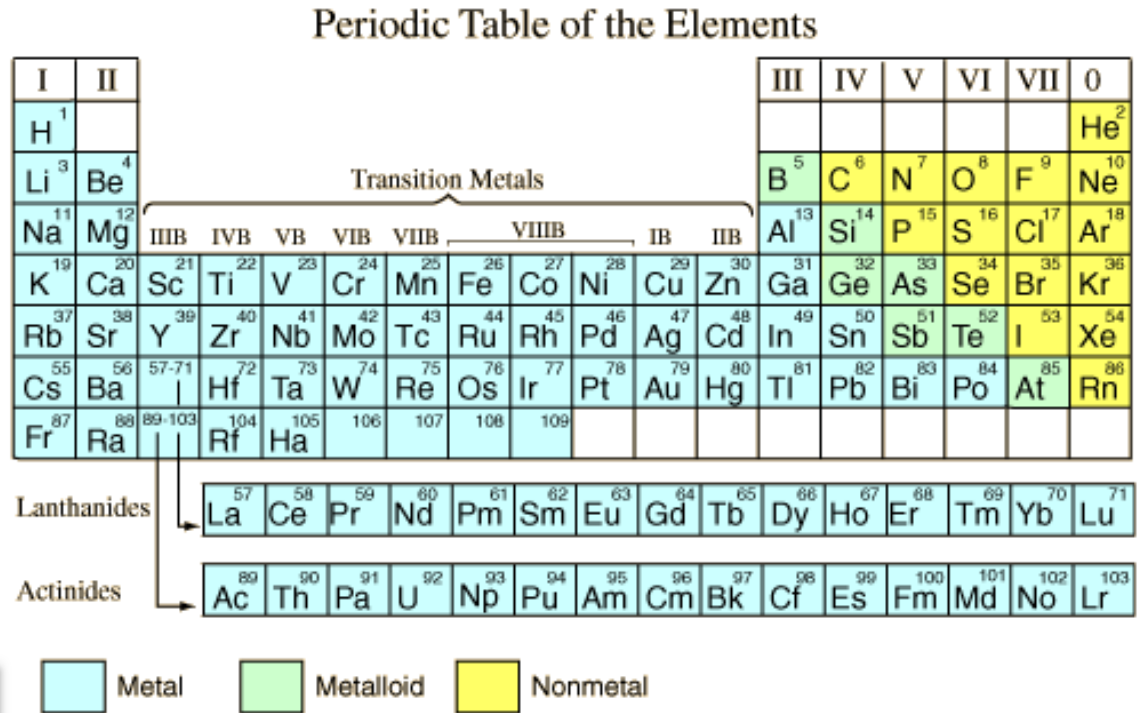
\includegraphics[scale=0.54]{ptable}
\end{center}
In this table, the elements are listed in columns in order of increasing atomic number. The columns represent groups of elements with similar chemical properties. The rows represent the periods, repeating patterns of groups. All the elements in a period have valence electrons in the same shell. The number of valence electrons increases from left to right in the period. When the shell is full, a new row is started and the process repeats.\\

There are two important principles that help us understand the chemical nature of atoms:
\begin{enumerate}[topsep=3pt,itemsep=-1ex,partopsep=1ex,parsep=1ex]
\item  Filled subshells are very stable. It takes a relatively large amount of energy to remove an electron and excite it to the next level. So atoms with filled subshells will be quite nonreactive.
\item Filled subshells are like hard spheres; they basically do not affect the chemistry of the atom. They are important for interactions with radiation, especially x-rays.
\end{enumerate}
The groups in the periodic tables can be summarized as the followings:
\begin{enumerate}[topsep=3pt,itemsep=-1ex,partopsep=1ex,parsep=1ex]
\item The noble gases (Column 0) occupy the last column of the periodic table, and have completely
filled shells. So under normal conditions they are monatomic gases and do not interact
with anything. They are nearly perfect atoms. 
\item  The $P$-subshell atoms (Column III through VII) are just to the left of the noble gases, and the are the halogens (F, Cl, Br, etc.). They lack just one electron. So they are violently reactive. As you move through the left through the p-subshell, this becomes less and less true.
\item The $S$-subshell atoms (Column I, II) are the leftmost columns of the periodic table and are the alkalis and the alkali earths. The alkalis have a single $s$ electron, making them highly reactive. Alkaline earths are still pretty reactive, because the second $s$ electron is pretty far from the nucleus. They are pretty good conductors for the same reason.
\item Transition metals are the elements where the d subshell is filling. Because these atoms are getting large and complex, there are some variations compared to what you might expect. For example, Cu ends up with a $4s^13d^{10}$ configuration instead of the expected $4s^23d^9$. This gives it a relatively free electron and makes it a much better conductor than we might expect.
\item Rare earths are pretty similar chemically to the transition metals.
\end{enumerate}

\subsection{Atomic spectra}
We will see spectral lines from absorption of photons when electrons are excited to higher energy levels. Those higher energy levels tend to be unstable, so the atoms may re-emit photons later. The wavelength of the emission may be different, depending on what de-excitation transition occurs. Example includes certain objects, including some scary animals, that will emit a blue glow under UV light.\\


\newpage
\section[Diatomic Molecules]{Diatomic Molecules}
Now we apply the theory to systems with more than one atom, that is, the molecules. In addition to the electronic energy levels that we have already studied, the nuclei can undergo various kinds of relative motion, such as vibrations and rotations. These motions, too, are quantized, so they lead to a more complex set of spectral features.\\

\subsection{Vibration states of molecules}
When two atoms are coupled by a spring-like force, near the bottom of the well, a quadratic potential is a good approximation. The solution to the Schrodinger equation has equally spaced energy levels:
\begin{align*}
E_N = hf\left( N + \frac{1}{2}\right)
\end{align*}
where $N$ is the vibrational quantum number, and $f$ is the simple harmonic oscillator frequency that satisfies the following:
\begin{align*}
f = \frac{1}{2\pi}\sqrt{\frac{k}{\mu}}
\end{align*}
with $k$ being a constant for a given system and $\mu$ being the system reduced mass:
\begin{align*}
\mu = \frac{m_1m_2}{m_1 + m_2}
\end{align*}
In fact, the potential has two terms, one is due to the electrons $V_e$. and one is due to the nuclei screened charges $Z_1,Z_2$:
\begin{align*}
V(r)= V_e(r) + \frac{Z_1Z_2}{4\pi \epsilon_0 r}
\end{align*}
where $r$ is the distance between the two atoms. To crudely estimate
the spring constant k, we will neglect the $V_e$ term. For small value approximation, we write the following:
\begin{align*}
V = \frac{1}{2} k r^2
\end{align*}
where the constant $k$ is estimated to be:
\begin{align*}
k \approx \left.\frac{d^2 V}{dr^2}\right|_{r=r_0} = \frac{e^2}{2\pi \epsilon_0 r_0^3} = \frac{(m_e c)^3}{4(\hbar c)^2}\alpha^4
\end{align*}
Note here we set $Z_1,Z_2$ to be approximately $e$. and $r_0$ to be twice the Bohr's radius. To estimate $f$, now we can write the following:
\begin{align*}
f = \frac{1}{2\pi}\sqrt{\frac{k}{\mu}} \leq  \Delta E_{\text{electron}} \sqrt{\frac{m_e}{\mu}}
\end{align*}
where $\Delta E_{\text{electron}}$ is the approximate scale of the atomic transition:
\begin{align*}
\Delta E_{\text{electron}} = m_ec^2 \alpha^2
\end{align*}
so the vibrational energy levels are smaller than atomic transitions by a factor given by:
\begin{align*}
\sqrt{\frac{m_e}{\mu}} \approx \frac{1}{100}
\end{align*}
We note here the vibration levels are uniformly spaced, and the selection rule for electric dipole transitions in harmonic oscillator potential requires $\Delta N = \pm 1$. 

\subsection{Rotational states of molecules}
The angular momentum of a system with angular speed $\omega$ is given by the following:
\begin{align*}
L = I\omega
\end{align*}
and hence the kinetic energy of the system:
\begin{align*}
K = \frac{1}{2}I\omega^2 = \frac{L^2}{2I}
\end{align*}
where we have seen quantization of the angular momentum:
\begin{align*}
L^2 = \hbar^2 l (l+1)
\end{align*}
From this simple analysis, we get the energy levels of the rotational states:
\begin{align*}
E_l = \frac{l(l+1)\hbar^2}{2I} = l(l+1)E_0
\end{align*}
where we see that the rotational energy levels are not uniformly spaced. Note here the selection rule applies $\Delta l = \pm 1$, and the energy of transition is given by:
\begin{align*}
\Delta E = E_{l+1}-E_l = (l+1) \frac{\hbar^2}{2I}
\end{align*}
We can estimate the size of energy levels using the rotational intertia of the molecule:
\begin{align*}
I = m_1r_1^2 + m_2 r_2^2 = \mu r_0^2
\end{align*}
where $\mu$ is the reduced mass and $r_0$ is the equilibrium separation. One can check that we obtain the following results:
\begin{align*}
\Delta E_{\text{electron}}\approx 10 \Delta E_{\text{vibration}} \approx  10000\Delta E_{\text{rotation}}
\end{align*}

Combining we obtain:
\begin{align*}
E_{Nl} = \left( N + \frac{1}{2}\right) hf + \frac{l(l+1)\hbar^2}{2I}
\end{align*}
and energy transitions must obey the same rules $\Delta N = \pm 1$, $\Delta l = \pm 1$. Therefore we have two cases in general:
\begin{align*}
\Delta E = 
\begin{cases}
hf + \hbar^2(l+1)/(2I) & \Delta N = 1,\text{ and }l\to l+1 \\
hf + \hbar^2 l/(2I) & \Delta N = 1,\text{ and }l\to l-1
\end{cases}
\end{align*}
In early 1940 two astronomers, Adams and McKellar, noticed spectral absorption lines in starlight coming from interstellar molecules. Two closely spaced lines $387.46\, nm$ and $387.58 \,nm$ were observed. This is in the UV region and was not caused by the CMBR. It was caused by the starlight. The former one is caused by starlight to excite from ground state to 1st vibrational level ($N=0,\, L=0 \ \to\ N=1,\,L=1$). And the later one corresponds to the same vibrational state but different  rotational state ($N=0,\, L=1 \ \to\ N=1,\,L=0$). This implies that some molecules are at a slightly higher energy levels. McKellar calculated the rotational energy of interstellar space to be $2 \,K$. Source of this thermal bath, the CMB radiation, became clear 25 years later.\\

\newpage
\section[Lasers]{Lasers}
Some forms of interaction between atoms and photons that we have seen so far include resonance absorption, photoelectric effect, and Compton scattering. Note here the resonance absorption is a phenomenon that an atom absorbs a photon of some appropriate frequency hence exciting the atom to an excited state. The excited atom might  spontaneously emits a photon with appropriate frequency and going back to a lower state, such process is called a spontaneous emission.\\

\subsection{Stimulated emission}
Here we will introduce another form of interaction between matter and radiation. The stimulated emission occurs when an excited atom absorbs a photon and emits multiple photons. Consider a sample of atoms in a thermal bath at temperature $T$, and assume that there are only two energy levels with ground state $E_1$ with number of atoms $N_1$ and an excited state which has number of atoms $N_2$. Denote $\Delta E = E_2 - E_1$. Since thermal equilibrium is assumed, then Boltzmann's result states that we have the following holds:
\begin{align*}
\frac{N_2}{N_1} = e^{-\Delta E/(kT)} = e^{-hf/(kT)}
\end{align*}
hTis equilibrium is dynamic, that is, atoms are continually jumping into the excited state and back down again. We are interested in the rates of absorption and emission. Let $B_{12}$ be the coefficient of stimulated absorption, let $A_{21}$ be the coefficient of spontaneous emission, and let $B_{21}$ be the coefficient of stimulated emission. Stimulated absorption or emission is due to thermal photons. Those photons, as we know, have a blackbody spectrum. The rate of absorption is proportional to the number of atoms in the ground state to begin with, as well as to the energy density of the surrounding radiation. Now we can write:
\begin{align*}
\frac{dN_{abs}}{dt} = N_1 B_{12} u(f,T) \qquad\qquad\qquad \frac{dN_{emiss}}{dt} = N_2(A_{21} + B_{21}u(f,T))
\end{align*}
In equilibrium, we must have:
\begin{align*}
\frac{dN_{abs}}{dt} = \frac{dN_{emiss}}{dt} \qquad \Rightarrow \qquad N_1 B_{12} u(f,T) =N_2(A_{21} + B_{21}u(f,T))
\end{align*}
We can solve for $u(f,T)$ from here and that must equal to the result from Planck's blackbody energy density:
\begin{align*}
u(f,T) = \frac{\frac{A_{21}}{B_{21}}}{\frac{N_2}{N_1}\frac{B_{12}}{B_{21}}-1} = \frac{\frac{A_{21}}{B_{21}}}{\frac{B_{12}}{B_{21}}e^{\frac{hf}{kT}}-1} = \frac{8\pi hf^3}{c^3}\left( \frac{1}{e^{\frac{hf}{kT}}-1}\right)
\end{align*}
whence:
\begin{align*}
\frac{B_{12}}{B_{21}} = 1 \qquad \qquad \qquad \frac{A_{21}}{B_{21}} = \frac{8\pi hf^3}{c^3}
\end{align*}
The ratio of spontaneous to stimulated emission grows like $f^3$. Thus, as $\Delta E$ increases, so does the relative fraction of spontaneous emission.\\

While spontaneous emission is independent of any incident electromagnetic radiation, in the stimulated emission process, a photon with energy $E_2 - E_1$ induces the emission of a photon from an atom in state $E_2$, causing it to make a transition to state $E_1$. The emitted photon is coherent with the first, that is, it has the same frequency, direction, and phase as the incident photon.\\

If we want to get more photons out than we absorb, we need to make $N_2>N_1$, and we achieve this via something called population inversion, using a metastable state suppressed by a selection rule.\\


We can use the principle of stimulated emission to produce  a  device  that produces  an  intense  beam  of  coherent  photons  by  stimulated  emission. Light Amplification by the Stimulated Emission of Radiation - LASER.\\


Microwaves have very long wavelengths, they have a low frequency, and therefore, are low energy. Masers are devices that emit coherent microwaves and are used in atomic clocks, extremely low-noise microwave amplifiers in radio telescopes, etc. An astrophysical maser is a naturally occurring source of stimulated spectral line emission. The emission is stimulated and monochromatic, the frequency corresponding to the energy difference between two quantum mechanics energy levels. This emission may arise in molecular clouds, comets, planetary atmospheres, stellar atmospheres, or various other conditions in interstellar space.\\

\subsection{Populated inversion}
Note from the above that the rate of stimulated emission from $E_2$ to $E1$ is proportional to the number ambient photons with energy $hf = \Delta E$. So it seems like we could greatly amplify number of photons of that energy through a kind of avalanche process: a photon strikes an atom in the excited state, inducing the
stimulated emission of a second photon of the same energy. These two photons strike two more atoms giving four photons. The problem is that, in thermal equilibrium, there are more atoms in the ground state than in the excited state. Moreover, since the coefficients of stimulated absorption and emission are equal, there will be more absorption than emission, and there will be no amplification of the field.\\


If we want to create more photons than we absorb, we need to make $N_2 > N_1$. This non-equilibrium situation is called a population inversion. We can do this if the state $E_2$ is relatively long-lived, that is, it is what we call a metastable state.\\

Here we gives one example of population inversion. A ruby rod is illuminated with high intensity light bursts. Some frequencies just right to excite the Cr atoms to bands of the pump levels. The chromium atoms de-excite radiationless to the metastable state at 1.79 eV. For a sufficiently intense flash, more atoms will end up in this state than remain in the ground state, and that gives population inversion.  When the atoms decay from this state, the resulting photons can stimulate additional decays. \\

The first laser ever built was a ruby laser build in 1960. Nobel prize in 1964 was awarded to Townes, Basov and Prokhorov for theoretical work on the maser-laser principle. This 3-level laser has some disadvantages: (1) it requires pumping more than half of the atoms out of the ground state to achieve population inversion, (2) the flash lamp produces a broad spectrum of light, so a lot of the energy is wasted, and (3) lasers need to be pulsed in order to let the crystal cool.\\

Another example of populated inversion. Helium has a pair of closely-spaced metastable 2s excited states $19.72\, eV$ and $20.61\, eV$. He atoms can be excited into these states through an electrical discharge through the gas, and these states are metastable because of the selection rule $\Delta l = \pm 1$. The neon atoms on the other hand have excited 5s and 4s states at
nearly the same energies as the two 2s states of the Helium, so they can be exited to 5s and 4s via collision with the helium atoms. The neon atoms, after being excited to the 5s and 4s energy states, can decay
readily to another excited state 3p, and immediately to an intermediate state at 3s via spontaneous emission, and eventually back to the ground state. The energy state 3p is normally unoccupied, hence the population in this state is smaller than that of the 5s and 4s states, we get a population inversion, and the stimulated emission between the 5s and 3p states gives the laser light at 632.8 nm.\\


\newpage
\section{Quantum Statistics}
We have been discussing simple systems, adding complexity as we go, in small steps: (1) H atom, (2) Multielectron atoms, and (3) Molecules. If we want to describe macroscopic systems, made of an Avogadro Number of particles, however, we need the tools from Statistical Physics. We are concerned how particles occupy a system which consists of several energy levels (and each energy level could also have several energy states). Today we are going to explore the key ways in which Quantum Mechanics modifies the classical statistical approach.\\

We often treat phenomena as if a single interaction occurs. For example: electron emitting light in a low density gas tube is treated as emission of one wavelength. However, in practical terms we often study cooperate phenomena, such as glowing tungsten filament, where individual atom would emit one frequency, all $10^{15}$ (or so) atoms involved emit white light. We cannot and don’t need 
to solve problem for $10^{15}$ atoms, but we can understand a complex 
system based on a few macroscopic variables (T, p etc). For example, 5 identical particles share 6 units of energy, in principle we can write down all the ways in each system how 
energy can distribute and calculate how often this happens. In practice this might become cumbersome but it turns out the probability to measure one particle with a certain energy follows an exponential distributions $e^{\beta E}$. The best known example is the Maxwell-Boltzmann energy  
distributions which describes gases under normal conditions. The most probable energy in the Maxwell-Boltzmann distribution is given by:
\begin{align*}
E_p = \frac{1}{2}kT
\end{align*}
with a mean energy:
\begin{align*}
E_p = \frac{3}{2}kT
\end{align*}
and one can use that to derive the Maxwell speed dsitribution with $E =mv/2$.\\

The Boltzmann distribution reads the following:
\begin{align*}
f_B(E) = e^{-\alpha}e^{-\frac{E}{kT}}
\end{align*}
and it provides the probability that a state of energy $E$ will be occupied. For the ideal gas with number density $n=\frac{N}{V}$, meaning $N$ particles in a volume $V$, the normalization constant is:
\begin{align*}
e^{-\alpha} = n\left( \frac{m}{2\pi kT}\right)^{3/2}
\end{align*}
To find the number of particles with energy $d E$ around $E$, we need to multiply the density of states, or the degeneracy:
\begin{align*}
n(E) \, dE = g_B(E)\, f_B(E) \, dE
\end{align*}
where $g_B(E)$ is the number of states, or the number of different ways that the system can have energy $E$.\\

A key property of particles in quantum mechanics is that they are 
indistinguishable. Main impact of quantum mechanics in statistical physics is that the Boltzmann distribution has to be replaced by two new equations to account for this fact. Indistinguishable here means that, while you can always distinguish the particles by their position if they are far enough apart, if they get too close to each other, their wave packets will overlap and you will no longer be able to tell which one is which. The de Broglie wavelength gives an order to define the closeness of two particles. Recall that there are two types of indistinguishable particles: (1) Bosons of integer spins (such as photons), and (2) Fermions of half-integer spins (such as electrons).\\

For Bosons, we have the Bose-Einstein distribution (BE):
\begin{align*}
f_{BE} = \frac{1}{e^{\alpha}e^{\frac{E}{kT}}-1}
\end{align*}
For Fermions, we have the Fermi-Dirac distribution (FD):
\begin{align*}
f_{FD} = \frac{1}{e^\alpha e^{\frac{E}{kT}}+1}
\end{align*}
where $e^{\alpha}$ is a system and temperature dependent normalization.\\

Note that the BE distribution predicts that at low energies the 
bosons tend to pack themselves together. We can illustrate this behavior with a two-particle system:
\begin{align*}
\psi_s(x_1,x_2) = \frac{1}{\sqrt{2}}\left( \psi_n(x_1) \psi_m(x_2) + \psi_n(x_2) \psi_m(x_1)\right)
\end{align*}
the probability of finding both bosons in the same state $n=m$ is given by:
\begin{align*}
P_{BE} = \psi_s^*\psi_s = 2\psi_n^*(x_1) \psi_n^*(x_2)\psi_n(x_1) \psi_n(x_2) = 2P_B
\end{align*}
Notice that the probability is twice higher than the classical MB distribution. It is as if the presence of bosons attract other identical bosons: the -1 term in the denominator of $f_{BE}$ results in an increased probability of finding multiple bosons in the same state.\\

In contrast, for fermions, we obtain:\begin{align*}
\psi_s(x_1,x_2) = \frac{1}{\sqrt{2}}\left( \psi_n(x_1) \psi_n(x_2) - \psi_n(x_2) \psi_n(x_1)\right)
\end{align*}
The presence of a fermion in a particular quantum state prevents 
any other identical fermions from occupying the same state. The +1 term in the denominator comes from the exclusion principle. For large energies both $f_{FD}$ and $f_{BE}$ approach $f_B$.\\

\subsection{Blackbody radiation from BE statistics}
This was the first application of the BE statistics, in which the Indian 
physicist Satyendra Bose used this distribution to derive Planck's formula. Bose sent his calculations to Einstein who was working on the same problem. Bosons were named after Bose by Paul Dirac. In order to retrace Bose's steps, we need to take the BE distribution:
\begin{align*}
f_{BE} = \frac{1}{e^{\frac{E}{kT}}-1}
\end{align*}
and compute the density of states $g(E)$. Write the probability as:
\begin{align*}
P(E) \, dE = g(E)\, f_{BE}(E)\, dE
\end{align*}
and compute the energy density:
\begin{align*}
u(E) \, dE = \frac{E\,P(E)}{L^3}\, dE
\end{align*}
Photons in a box are standing waves, modes, and energies. \\
Here we can write the following :
\begin{align*}
p= \frac{\hbar \pi}{L}\sqrt{n_x^2+n_y^2 + n_z^2} \qquad\qquad E = pc = \frac{\hbar c\pi}{L}\sqrt{n_x^2 + n_y^2 + n_z^2}
\end{align*}
the number of states between $E$ and $E + dE$ is $1/8$ of the volume of a spherical shell with radius $r = n$ and $r=n+dn$. That is, we write:
\begin{align*}
g(n) \, dn = 2 \cdot \frac{1}{8}\cdot 4\pi n^2 \, dn
\end{align*}
where the factor $2$ comes from polarization. Then with the fact that $E = \frac{\hbar c\pi}{L}n$, we get:
\begin{align*}
dE = \frac{\hbar c\pi}{L} dn
\end{align*}
combining we get:
\begin{align*}
P(E) \, dE = g(E) \, f_{BE}(E)\, dE = \pi \left( \frac{L}{\hbar c\pi}\right)^3 \, \frac{E^2}{e^{\frac{E}{kT}}-1}\, dE
\end{align*}
The energy density $u(E)$ is the energy, times the probability that a 
photon will have that energy, divided by the volume, hence we get:
\begin{align*}
u(E) \, dE =  \pi \left( \frac{1}{\hbar c\pi}\right)^3 \, \frac{E^2}{e^{\frac{E}{kT}}-1}\, dE
\end{align*}
using $E = \hbar \omega = hc\lambda$, we obtain the Planck's Formula. \\

Planck derived his formula assuming Maxwell-Boltzmann statistics applied to a gas of distinguishable particles. We've now obtained the same result using Bose-Einstein 
statistics applied to indistinguishable particles. This does not always work, but in this case it illustrates the wave-particle duality of photons.\\

We saw an example of the Bose-Einstein statistics. For Fermi-Dirac, systems of spin-1/2 particles are found throughout nature, so the their distribution explains a lot and is 
important in many systems we will encounter: (1) Electrons in metals, the electron degeneracy pressure that holds up a white dwarf 
star, as well as the neutron degeneracy pressure that supports 
a neutron star. (2) The distribution of relic neutrinos from the Big Bang (just as the distribution of relic photons, which have spin-1, is described by the blackbody formula, which follows from BE statistics).
(3) Nuclear energy levels, as nuclei are comprised of spin-1/2 protons and neutrons.\\ 

\subsection{The use of classical statistics}
We expect that when the particle spacing is large compared to the de Broglie wavelengths, classical statistics is applicable. The de Broglie wavelengths is given by:
\begin{align*}
\lambda = \frac{h}{p} = \frac{h}{\sqrt{2m E_k}} = \frac{h}{\sqrt{2m(3kT/2)}} = \frac{h}{\sqrt{3m kT}}
\end{align*}
On the other hand, the average spacing of particles is of order $( V/N)^{1/3}$, hence the criteria for being able to use classical statistics is that we have:
\begin{align*}
\frac{N}{V}\frac{h^3}{(3mkT)^{3/2}} \ll 1
\end{align*}


\hfill\break
\hfill\break
\hfill\break
\begin{center}
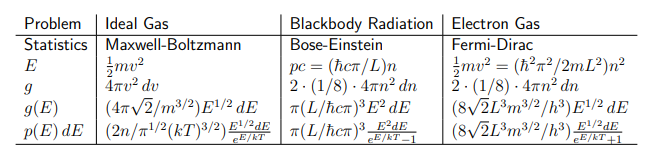
\includegraphics[scale=1]{StatEX}
\end{center}
\newpage
\section{Electrons in Metals}
We have seen how quantum mechanics impacts the statistical behavior of particles. Depending on their spin, bosons and fermions follow different statistics. We have worked out one application, that the blackbody radiation formula was derived considering a gas of photons following the Bose-Einstein statistics. Now we look into an application from the field of solid state physics. \\

\subsection{Specific heat}
Specific heat is the change in thermal energy per mole per unit change in temperature. Classically, we can think of atoms in a solid as a system of many coupled 3-d harmonic oscillators. That implies 6 degrees of freedom, three for kinetic, and three for potential. From the equipartition theorem we have $kT/2$ of energy per degree of freedom. Thus, we can write:
\begin{align*}
E = \frac{6N_AkT}{2} = 3N_AkT = 3RT
\end{align*}
where $N_A$ is a Avogadro number. The specific heat is then given by:
\begin{align*}
C_V = \frac{dE}{dT} = 3R = 24.9\, J/(mol\cdot K)
\end{align*}
We see that this prediction, called the Dulong-Petit predictions seems to agree with the data only in the special case of solids at high enough temperatures. The problems with the classical picture is that the classical result (Dulong-Petit), is valid for solids at room temperature, but at temperatures below a certain threshold (such threshold is different for each material) the observed heat capacity falls to zero. Since metals have free-ranging electrons that insulators do not have, they should have extra degrees of freedom, and therefore, classically speaking, a higher heat capacity than insulators. However, this not observed. We will see how the quantum theory solves these puzzles.\\

Vibrations of the solid are akin to harmonic oscillators. Their energy must be quantized, similar to photons, they are called phonons.
A phonon is the elementary excitation in the quantum mechanical treatment of vibrations in a crystal lattice or the quantum unit of a crystal lattice vibration. For simplicity, we assume that solids can oscillate at onely one frequency $\omega$. Hence this mode can only assume energy values $n\hbar \omega$ for $n \in \N$. The average energy for each phonon is given by:
\begin{align*}
\langle E\rangle= \frac{\hbar \omega}{e^{\hbar \omega/(kT)}-1}
\end{align*}
there are $3N_A$ oscillators, so one can write:
\begin{align*}
E = 3N_A\langle E\rangle=\frac{3N_A\hbar \omega}{e^{\hbar \omega/(kT)}-1}
\end{align*}
and that the capacity is given by:
\begin{align*}
C_V = \frac{dE}{dT} = 3N_Ak\left( \frac{\hbar\omega}{kT}\right)\frac{e^{\hbar \omega/(kT)}}{(e^{\hbar \omega / (kT)}-1)^2}
\end{align*}
note here we have $C_V \to 0$ as $T\to 0$, and we have $C_V \to 3N_A kT = 3R$ as $T \to \infty$, agreeing with the classical picture. This theoretical insight was first devised by Einstein who realized that the oscillations, and not only the atoms, should obey the Bose-Einstein statistics. Einstein's model is oversimplified in assuming a single frequency for all oscillations. Peter Debye refined the theory later, assuming a distribution of frequencies similar to a black body radiation. Debye's refined model fits the data with great precision.\\

Now, we know that metals contain a large number of free electrons that are responsible for their widely varying electrical properties, while insulators contain very few such electrons. Yet it turns out that the classical Dulong-Petit law is obeyed in the appropriate temperature regime  by both conductors and insulators, the  electrons  do not  seem  to  play  a  role in the heat capacity. An explanation to that is the fact that electrons are Fermions, unlike phonons, they obey the Fermi-Dirac statistics. Moreover, electrons in a solid are like particles in a box, and the energy levels are given by:
\begin{align*}
E_n = \frac{\hbar^2 \pi^2}{2mL^2}(n_x^2 + n_y^2 + n_z^2)
\end{align*}
where $L$ is the characteristic length of the box, and $n_x^2 + n_y^2 + n_z^2 = n^2$ is the number of energy level states that are available. The probability of finding an electron with energy between $E$ and $E+dE$ is given by:
\begin{align*}
P(E) \, dE = g(E) \, dE \cdot f_{FD}(E)
\end{align*}
The number of states of energy between $E$ and $E+dE$ is the same as the volume of spherical shell with radius $n$ and $n+dn$. We only include $1/8$ of the sphere because $n$ must be positive. And include a factor of two because the projection of spin on $z$-axis can be plus or minus $1/2$. So, we have:
\begin{align*}
g(n)\, dn  = 2\cdot\frac{1}{8}\cdot 4\pi n^2 \, dn
\end{align*}
We now obtain:
\begin{align*}
n(E) = \frac{(2m)^{1/2}L}{\hbar \pi}E^{1/2}\qquad\qquad dn = \frac{1}{2}\frac{(2m)^{1/2}L}{\hbar \pi}E^{-1/2}\, dE
\end{align*}
combining we get:
\begin{align*}
g(E) \, dE = 2\cdot \frac{1}{8}\cdot 4\pi \left( \frac{2mL^2}{\hbar^2 \pi^2}\right) E \cdot \frac{1}{2}\cdot \frac{(2m)^{1/2}L}{\hbar \pi}E^{-1/2}\, dE = \frac{8 \sqrt{2}\pi L^3 m^{3/2}}{h^3}\, E^{1/2}\, dE
\end{align*}
and hence we have:
\begin{align*}
P(E)\, dE =  \frac{1}{e^{(E-E_F)/kT}+1}  \frac{8 \sqrt{2}\pi L^3 m^{3/2}}{h^3}\, E^{1/2}\, dE 
\end{align*}
note here we used the fact that we can rewrite the Fermi-Dirac distribution as:
\begin{align*}
f_{FD} = \frac{1}{e^\alpha e^{E/(kT)}+1}\qquad\qquad \text{with }\alpha = -\frac{E_F}{kT}
\end{align*}
and here $E_F$ is called the Fermi Energy.\\ Now we need to normalize the probability by finding $E_F$:
\begin{align*}
N = \int_0^\infty P(E)\, dE
\end{align*}
Note that, at $T=0$, because the electrons are Fermions and they cannot occupy the same energy levels, so they will occupy energy levels up to the Fermion energy level. All those states must be fully occupied. Moreover, there are zero electrons in any state above that, and so we can write:
\begin{align*}
N = \frac{8\sqrt{2}\pi L^3 m^{3/2}}{h^3}\int_0^{E_F}E^{1/2}\, dE \qquad \Rightarrow \qquad E_F = \frac{h^2}{2m}\left( \frac{3N}{3\pi V}\right)^{2/3}
\end{align*}
At finite temperature, the distribution is smeared out, we have an area near $E_F$ with a width on the order of $kT$ within which electrons can gain or lose energy. Only a very small percentage of electrons are this close to the Fermi surface. For a typical metal, with around one free electron per atom, Fermi energy is much greater than room temperature, with oder a few eV, which is given by several thousand degrees Kelvin. Therefore, the free electrons do not play a role in the heat capacity. 
Typically the amounts of thermal energy getting put into a solid when you heat it up are on the order of $kT$. But, due to the exclusion principle, very few electrons have an accessible state within $kT$ of them, only those within $kT$ or so of the Fermi surface have a chance to absorb it. \\

\subsection{Electrical conductivity}
A similar principle governs electrical conductivity. Only few electrons close to the Fermi surface contribute. However, our classical kinetic intuition that electrons as particle accelerated in $\vec{E}$-field and  acceleration constant until scattering on Ion, fails even worse. Classically,
drift velocities are overestimated,
temperature dependence wrong,
and we do not know whether a material is a conductor or not in the first place. Even taking into account FD statistics fixes only some of these issues. We have to consider the wave-nature of electrons, along with FD statics, not a kinetic theory. \\

The calculations from classical theory are given by the followings:
\begin{align*}
v_d = \frac{eE}{m}\tau \qquad\qquad\qquad \lambda = \frac{1}{n_a \pi r^2}
\end{align*}
where $v_d$ is the drift velocity of the electrons in the material that directly contribute to the current flow, which comes from the additional, non-random piece that gets added to the velocity by the applied electric field. $\lambda$ is the mean free path of the electrons. Here $r$ is a typical atomic radius, $\tau$ is the average time between collisions between the electrons and the atoms they encounter, $n_a$ is the number density of atoms, and $E$ is the external electric field. This result is not correct by the facts that (1) the numbers, such that conductivity, that emerge from this theory do not agree with the data, (2) this theory predicts an incorrect dependence on temperature, and (3) this theory does not predict why a given material conducts electricity, and it does not  tell us why certain materials are conductors, others are insulators, and others are semiconductors.\\


Quantum mechanically, our picture of the electron as being a ping-pong ball bouncing off bowling-ball atoms in the material should be replaced by an electron wave scattering off the regular arrangement of ions in the lattice. For de Broglie wavelengths longer than the crystal spacing, which is what we have here, Bragg scattering cannot occur. In fact, in a perfectly-ordered crystal lattice, no scattering takes place. Scattering of electron waves is entirely due to imperfections and defects in the lattice. These are due mainly to (a) impurities, and (b) thermal motion of the ions. The final results is obtained via FD statistics and considering the wave nature of electrons as described above:
\begin{align*}
\lambda = \frac{1}{n\pi \langle r^2\rangle} = \frac{M\omega^2}{2\pi nk}\frac{1}{T}
\end{align*}
where $n$ is the number of free electrons per unit volume.

\subsection{Band structure of solids}
We have discussed the problem of the motion of electrons in metals using the tools of quantum statistical physics. In particular, we showed that the role of free electrons in the specific heat conductivity of solids is none. Now we are going to look deeper into the world of solids and attempt to answer the question: What makes something a good electrical conductor,  rather  than,  say,  an  insulator? In order to answer this question, we will first establish the concept of electrical conductivity. Then we will discuss what happens with the atomic energy levels when atoms are placed close to each other.\\

Electrical conductivity arises from the motion of free electrons. Those key ideas can be summarized as the followings:
\begin{enumerate}
\item Drift velocity. Current flow comes from a small (10-5 m/s) drift velocity, which has a net direction to it, superimposed on the much larger but randomly directed thermal velocity of the electrons.
\item Mean free path. The average distance the electrons go between scattering off the atoms in the lattice. This is what determines the drift velocity, because in between scatterings the electrons experience constant acceleration from the applied electric field.
\end{enumerate}

In Quantum mechanics, the scattering of the electron is described as a wave function propagating in a periodic lattice. For such a system, the particle has periodic potential, and the solution of Schrodinger's equation is:
\begin{align*}
\psi_k(x) = u_k(x) e^{ikx}
\end{align*}
where $k$ is real, and the function $u_k$ has the same periodic feature of the potential. Note that this function is not attenuated, this means that for this idealized lattice the mean free path is infinite.\\

In real systems, we have two more effects to consider. (1) Impurities, they play a dominant role only at very low temperatures. (2) Thermal motion, when the atoms are all wiggling randomly, the lattice is no longer perfectly periodic. An analogy here is that we can imagine walking down a street with an open manhole every 5 feet. You can adjust your stride to exactly match that spacing and never fall in, your mean free path is infinite. As a result, the electron wave are scattered off the imperfect-periodic arrangement of ions in the lattice.\\



We saw what happens when we bring two H atoms close to each other. Their electrons are described by a two-particle wavefunction. The total wavefunction for a two-electron system is described by the following:
\begin{align*}
\psi = \psi_{\text{spatial}} \cdot \psi_{\text{spin}}
\end{align*}
While the total wave function must be anti-symmetric, the spatial part of the wavefunction can be either symmetric or anti-symmetric, because of the two possibilities for the electron spins.\\

The spatial wave function for the two-electron system can be made symmetric or antisymmetric via the following:
\begin{align*}
\psi(x_1,x_2) = \frac{1}{\sqrt{2}}\left( \psi_1(x_1) \psi_2(x_2) \pm \psi_1(x_2) \psi_2(x_1)\right)
\end{align*}
where $\psi_1$, $\psi_2$ are wave functions for single-electron system. For the spatial wave function of a single electron, we can think of the two-atom configuration as the molecular bounding in a diatomic hydrogen
molecule, where the two protons in the system serve as two finite wells, or the two potentials that confine an electron. An electron in such a two-well system can travel in such space and its position is characterized by its wave function. There is a nonzero probability that the electron
can tunnel from one of the wells to the other, but such a probability is small enough to be neglected when the wells are separated far away. The wave functions of the single electron, that is the solutions to the Schrodinger equation in such configuration, can be symmetric and antisymmetric. When the two wells are far apart, the energies of each pair of symmetric-antisymmetric wave functions degenerate, but when the wells are brought near together, the degeneracy is lifted, hence resulting in the split of energy levels of the electron. The antisymmetric wave function in this case has energy higher than the symmetric one.\\

We now have what would otherwise have been two states of the same energy being split into different energy levels: lifting a degeneracy. Now imagine what happens when one has N atoms together. The energy levels will smear out into a band with well defined upper and lower bounds — that's band theory in a nutshell. In the following figure, the energies of the 3s level of the multiple-atom system for (1) two atoms, (2) five atoms, (3) large amount of atoms, are depicted.
\begin{center}
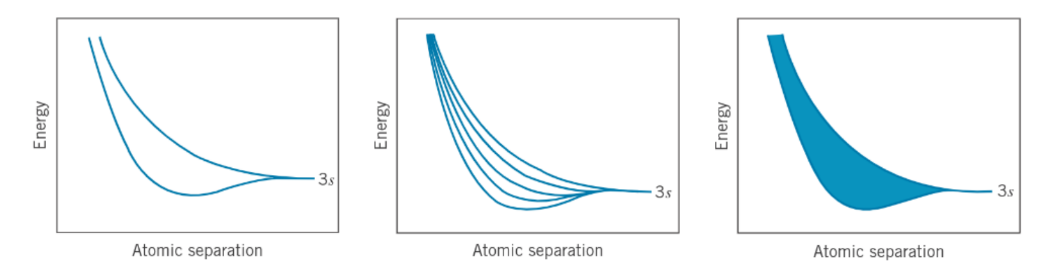
\includegraphics[scale=0.68]{bandStruc}
\end{center}
For large amount of atoms, there are so many energy levels, or orbits, that they become continuous. Note that there are $2(2l+1)N$ electrons per band, where $N$ is the number of atoms. That is, bands are composed of closely spaced orbits. Different atoms have different atomic spacing, and that is the fundamental reason why some materials are conductors some are insulators.
\begin{center}
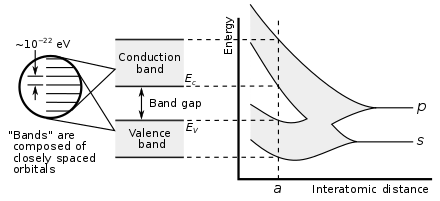
\includegraphics[scale=0.8]{BandGap}
\end{center}

\subsection{Conductors and insulators}
For Na atom ($1s^22s^22p^63s^1$), at the ground state, the first two shells and the corresponding three subshells are completely filled. However, the 3s level could hold $2$ electrons, while only one electron presents in the 3s level, so this level is half empty. At $T=0$, all occupations up to $E_F$ are filled, and the probability above $E_F$ is zero. For $T> 0$, the states above $E_F$  have probabilities now that are non-zero, hence there is situation where the $2p$ band being partially full and $3p$ band being partially filled. Here $E_F$ is in the middle 3s band, so we typically say 3s a conduction band for Na as $E_f$ sits right at that band.\\

When $E_F$ sits exactly between two bands, that is exactly at the band gap, then the material tends to be an insulator. Many electrons in valence band but few empty states to move through. Conversely, if there are many states in the conduction band but only a few electrons occupying that conduction band, the material has good conductivity. Conventionally, the top most band is usually called the conduction band, and those bands that are filled are called the valence bands. 
\begin{center}
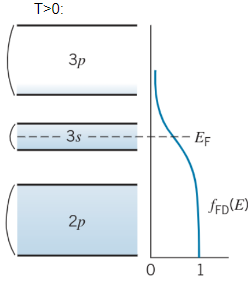
\includegraphics[scale=0.88]{bands1}\qquad\qquad\qquad
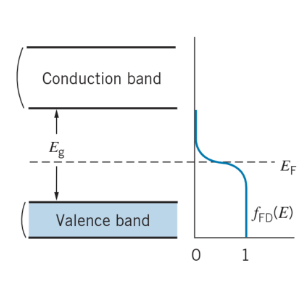
\includegraphics[scale=0.88]{bands2}
\end{center}


The electron moving through the lattice is a scattering problem. At each point of interaction, the electron can be modeled as an incident wave plus a reflected and transmitted wave. For those special values of $\lambda$ when reflected waves from adjacant ions are in phase, that is $n\lambda = 2a$, so called the Bragg condition for scattering in $1$-dimenson,  where $a$ is the spacing between ions in the lattice, we get constructive interference between reflective and incident waves forming standing waves, in other words, such condition is given by:
\begin{align}
ka = \pm n \pi
\end{align}
For the case where $k = \pi /a$, we have two types of standing waves:
\begin{align*}
\psi_1 = \sin(kx) = \sin(\pi x/a) \qquad\qquad\qquad \psi_2 =\cos(kx) = \cos(\pi x/a)
\end{align*}
If one consider the ions sit at the $x$-axis with spacing $a$ and one of them is placed at the origin, then we see here $\psi_2$ gives a higher electron density near the ion sites than $\psi_1$. The difference in potential energies corresponds to the magnitude of the energy gap, and the set up of standing waves at $k$ given by (17) implies that traveling waves cannot exit for these $k$. Therefore, we get an energy dependence on $k$, which leads to emergence of bands. In $3$-dimensional, the situation is more complicated, but the same principle apples. 
\begin{center}
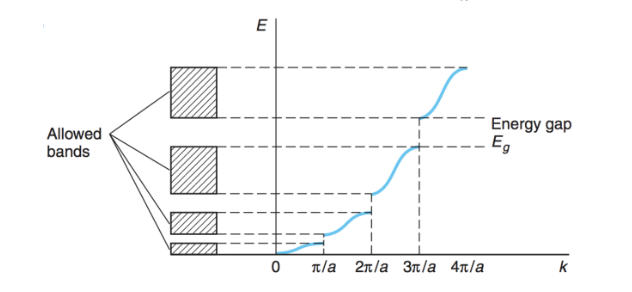
\includegraphics[scale=0.9]{allowedBands}
\end{center}

In general, energy levels which are lines in atoms become energy bands in solids. A consequence of this is that solids will be good conductors or insulators depending on the occupancy of the outermost band. Metals are good conductors because they have the conduction band partially full, meaning that electrons can be easily excited by a modest voltage. Insulators are poor conductors because their outermost band is a valence band, so electrons could only rise to the conduction band if the applied voltage is large enough to overcome the large energy gap between the bands. \\

\subsection{Semiconductors}
The Fermi-Dirac distribution is a sharp step function at $T=0$. At higher temperatures, however, it is smooth. Consider the case where Fermi energy $E_F$ lies in a band gap. If the energy gap is small, this smooth distribution means that a small, but non-zero, number of electrons may be excited to cross the gap. For a $1\,eV$ gap and a Fermi Energy that lies about in the middle of the gap, which is typically the case for semiconductors, we expect 1 atom per billion contributing to the conduction band.\\

Those electrons come from the valence band, leaving behind unoccupied states called holes. These holes act very much like real particles; you can think of the absence of negative charge in a certain location as being equivalent to the presence of positive charge there. So when we apply a voltage to this semiconductor, current will
flow, electrons in one direction and holes in the other. It sounds like you might get no net current this way, but the electrons usually turn out to be more mobile than the holes, so there is an overall nonzero current flow. This picture presents us with both a problem and an opportunity. The problem is that the action here involves one per billion electrons. So the behavior of semiconductors is very sensitive to impurities. This is also the opportunity. By introducing impurities in a controlled way, a process known as doping, we can exert a fine level of control over the electrical properties of the material.\\

The silicon atom has four valence electrons, and forms covalent bonds with four of its neighbors in a crystal. Now imagine replacing a few of the Si atoms with an atom with five valence electrons, such as arsenic, these left over electrons are loosely bound and are easily
excited to the conduction band. They occupy discrete, hydrogen-atom-like energy levels called donor levels that lie just below the conduction band. Such a material is called an n-type semiconductor because the charge carriers are negative. The addition of an n-type impurity greatly increases the conductivity; the addition of just a few parts per million of arsenic can increase the conductivity by several orders of magnitude.\\

Alternatively, we can dope the material with an element with three valence electrons, such as gallium. The gallium atom accepts electrons from the valence band of Si to complete its outer shell, thus creating a vacancy in the Si's valence band. The impurity creates empty levels, called
acceptor levels just above the valence band that are due to the holes from the ionized gallium. When these are filled, the resulting holes in the valence band act like positive charge carriers. Such a material is called a p-type semiconductor because the charge carriers are positive.\\


The number of donated electrons in a doped n-type semiconductor, or holes in a doped p-type semiconductor, is typically much greater than the intrinsic number of electron-hole pairs created by thermal excitation of electrons from the valence band to the conduction band. In an electric field, the current will consist of both majority (donor) carriers and minority (intrinsic) carriers.\\


Really interesting things start to happen when you put n- and p-type materials together. The boundary region is called a pn-junction. When p-type and n-type material come into contact, the n-type stuff sees available holes, and the p-type stuff sees available electrons to fill the acceptor states. So electrons diffuse across
the junction from the n-side to the p-side until equilibrium is established. In between the n- and p-type regions, there are not many charge carriers of any type, and so the junction has a high resistance. This transition area near the junction is called the depletion region.\\


Now imagine hooking this system up to a battery. If we put the positive side of the battery on the p-side, we lower the potential across the junction. This means
that electrons can flow again from the n-side to the p-side. Alternatively, imagine putting the negative side of the battery on the p-side. Now we have raised the potential difference between the two sides, so current can not flow. We see that we have a device that can only conduct current in one direction. Such a device is called a diode, and such phenomenon is called the forward/reverse biasing. Hence a diode acts like a check valve for current. It conducts current only in one direction.\\

Diodes are very important elements for modern electronics. In the case of Light Emitting Diode (LED), the external current supplies energy to excite electrons to conduction band. When they fall back they emit light. Stimulated emission is also employed in this process. \\

Transistor joins two diodes back to back, and it either amplifies a current or switch it on/off. It can be used to create logic gates, hence has lots of applications in making integrated circuits and CPU.
Transistor was invented 1948 by Bardeen, Brattain and Schockley in 1948 (Nobel 1956), and it was a revolution in the world of electronics, resulting in a multi-billion dollar industry.\\

\subsection{The quantum Hall effect}
If the charge carriers are electrons, the magnetic force will cause them to move up to the top of the strip, leaving the bottom of the strip with an excess positive charge. This will continue until the electrostatic field $E$ caused by the charge separation produces an electric force on the charge carriers just balancing the magnetic force.
If the charge carriers are positive holes, the overall picture is the same except that the sign of $E$ will be reversed. The resulting potential difference is the Hall voltage:
\begin{align*}
V_H = Ew = v_d B w
\end{align*}
where $v_d$ is the drift velocity of the charge carriers, and $w$ is the width of the strip. The Hall effect is used to determine carrier density, electrical resistivity, and the mobility of carriers in semiconductors.
It can also be used to measure magnetic field strengths using a calibrated metal strip, measuring the Hall voltage then yields the value of $B$.\\

Some basics about the quantum Hall effect. The electric field is perpendicular
to the applied magnetic field $B$ and, as a result, the charge carriers move in a circular path, or orbit, of radius $r = mv/(qB)$. The fact that electrons obey the Pauli exclusion principle prevents
the orbits from overlapping and determines how closely the electrons can group together on the negative side of the sample. Recalling that the orbital motion of electrons is quantized with only certain radii being allowed (those for which the orbit circumference equals an integral number of de Broglie wavelengths) we know that increasing the magnetic field decreases the orbit radius, but such decreases must occur suddenly and result in another, smaller allowed radius. Thus, more electron orbits can fit without overlapping in a given area and the density of charge carriers increases on the edges of the semiconductor sample. This increases the frequency of collisions and hence the Hall resistance. Since the orbit radii change only in quantized steps, so must the
Hall resistance. \\

In the 1980s, while studying the Hall effect in thin semiconductors at very low temperatures and very large magnetic fields, Klaus von Klitzing discovered that the Hall voltage is quantized. The quantization of the Hall voltage is due to the quantization of the Hall resistance:
\begin{align*}
R_H = \frac{V_H}{i} = \frac{R_K}{n}
\end{align*}
where $i$ is the current, and $n\in \N$, and $R_K$ is the von Klitzing constant:
\begin{align*}
R_K = \frac{h}{e^2} \approx 25.831\, \Omega
\end{align*}

Soon after, Tsui, Laughlin and Stormer, while investigating the quantum Hall effect in ultra-pure semiconductors, discovered quantized values of the Hall resistance for values of $n$ that were rational fractions formed from small integers. \\

Two nobel prizes were awarded for discoveries of the Quantized Hall effects: (1) 1985 - von Klitzing, and (2) 1998 - Laughlin, Stormer, Tsui.



\subsection{Superconductors}
In 1911, the Dutch physicist Heike Karmelingh Onnes discovered that the resistance of mercury suddenly dropped to zero when the sample was placed below a critical temperature of about 4.2K. That is close to the liquefying temperature of Helium, which Onnes himself had discovered how to make in his lab circa 1908. Onnes won the 1913 Nobel prize. The discovery of superconductivity is an example of how technical breakthroughs, which can give the ability to achieve new extreme conditions, often lead to discoveries of fundamental importance. 
In the following, we will discuss how  this superconductivity can be explained.\\

The presence of a magnetic field lowers the critical temperature for superconductivity. In fact, above a certain critical field, there is no superconductivity at all. It may take very low temperatures and sometimes high pressure, but there are many materials for which superconductivity has been observed. For a few notable examples: Niobium and Titanium compounds, which are used in MRI imaging machines. In 1986, Bednorz and Muller discovered an exotic compound of lanthanum, barium, copper, and oxygen that superconducts at $30\,K$.
They won the 1987 Nobel for their discovery of the first high-temperature superconductor. A year or so later, it was discovered that yttrium-barium-copper-oxide would superconduct at $92\, K$. This one is very important because it is warmer than liquid nitrogen, which liquifies at $77\, K$ and is cheap and easy to make compared with liquid helium.\\

Although we tend to think of superconductors as being defined by their electrical properties,
their magnetic properties are at least as interesting. We note that $E$-field inside a superconductor is zero because it has zero resistance and hence zero emf. Recalling that we have:
\begin{align*}
\nabla \times \vec{E} = -\frac{\pd \vec{B}}{\pd t}
\end{align*}
we find that, the magnetic field inside conductor is constant. When the  superconductor is cooled below the critical temperature in an external magnetic field, a screening current at the surface produces a field that cancels the external magnetic field perfectly. So, that constant magnetic field inside the conductor is zero. That is, superconductors expel external magnetic fields, called the Meissner effect.\\

Only a subset of materials, known as Type-I superconductors, exhibit the complete Meissner effect for fields below a critical value. There are also Type-II superconductors, which have two critical field values and can form flux tubes. In the Type-II superconductors, exxternal magnetic field lines can penetrate the material but are confined to flux tubes of normally resistive material. \\

In 1957, John Bardeen, Leon Copper, and Bob Schrieffer published a successful theory of superconductivity, now known as the BCS theory (1972 Nobel prize). Their theory states that electrons in a superconductor are coupled in pairs, called Cooper pairs, at low temperatures. The coupling comes about because of the interaction between electrons and phonons in the crystal lattice. A pair of electrons close at $T_C$ will form a Cooper pairs through interactions with the crystal lattice. This pairing results from a slight attraction between the electronics related to lattice vibrations. \begin{center}
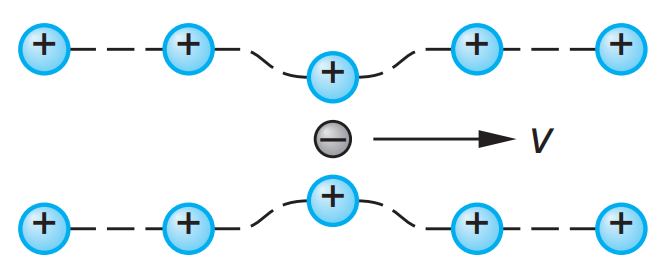
\includegraphics[scale=0.35]{BCSTheory}
\end{center}
The figure illustrates an electron traveling through the lattice of positive ions and generates a wave of increased charge density, and the wave can be encountered by a second electron and forming an attraction between two electrons. This is a rather strong interaction in contrast to classical conduction. The motions of all of the Cooper pairs within a single superconductor are correlated, and each Cooper pair constitutes a system that functions as a single boson, hence different pairs can have same energy state. Application of an electric voltage moves all Cooper pairs, constituting a current.\\

The theory predicts that the energy required to break a Cooper pair is given by:
\begin{align*}
E_g = 3.5k T_c
\end{align*}
and the dependency between $T$ and $B$ is given by:
\begin{align*}
\frac{B_c(T)}{B_c(0)} = 1-\left( \frac{T}{T_c}\right)^2
\end{align*}
where $B_c$, as a function of temperature, is the critical magnetic field for which superconductivity of the material can occur. \\

Now consider a superconducting loop. There can be a magnetic flux through the loop due to the current in the loop. 
According to Faraday's law of induction, if the flux changes, an emf will be induced in the loop that is proportional to the rate of change of the flux. But for a superconductor, there can be no emf in the loop because there is no resistance. 
Therefore, the flux through the ring cannot change. The quantum-mechanical treatment of superconductivity (the BCS theory) reveals that the total flux through the loop is quantized:
\begin{align*}
\phi_m  = n\frac{h}{2e}\qquad\qquad n \in \N
\end{align*}
We note that each flux tube in a type-II superconductor contains one quantum of flux.\\


\newpage
\section{Nuclear reactions}
\subsection{Radioactivity}
In 1896 Henri Becquerel left accidentally a piece of potassium uranyl sulfate on a wrapped photographic plate, nevertheless he later found that the plate had been exposed. The term radioactivity was coined by Marie and Pierre Curie. The Curies shared the 1903 Nobel Prize in physics. Marrie Currie was the first woman to win a Nobel, and she also won a Nobel Prize in Chemistry in 1911, making her the first person, and only woman to win twice, and only person to win in 2 sciences. Their daughter, Irene, won a Nobel Prize in Chemistry. in 1935. \\

Radioactivity is the spontaneous emission of radiation. The nucleus has a collection of positive charges. They are bound together by a force that, at such small distances, is strong enough to overcome their Coulomb repulsion. There are limits for how many protons and neutrons you can put in a nucleus. Therefore, only around 250 of the thousands of isotopes are stable. Half-life refers to the time it takes for a sample to decay to half of its original amount. If the sample has $N(t)$ amount, with $N_0$ being the amount at time $0$, and the sample is allow to decay at a rate $\lambda$, then we write:
\begin{align*}
-\Delta N = \lambda N \Delta t \qquad \Rightarrow \qquad \frac{dN}{dt} = -\lambda N(t) \qquad \Rightarrow \qquad N(t) = N_0e^{-\lambda t}
\end{align*}
Decay constant $\lambda$ is the constant parameter in the exponential decay formula and is given in units of 1/time. Mean lifetime is time it takes for the sample to be reduced to $1/e$ of its original size, defined as the inverse of the decay constant. Half-life is time it takes for half the sample to decay. \\

Another exponential law takes place when we consider the penetration of particles in a material:
\begin{align*}
N(x) = N_i e^{-\mu x}
\end{align*}
Here the constant $\mu$ is the attenuation coefficient, which has units of 1/length. The distance associated with the attenuation coefficient is where the number of particles is reduced to 1/e of its original number. \\

\subsection*{Alpha Decay}
All nuclei with $Z>83$ suffer alpha decay. Their half lives range to 10 ns to billions of years. The radiation is highly ionizing and poorly penetrating, which means it has a high $\mu$. Alpha particles are composite particles consisting of two protons and two neutrons tightly bound together. Nuclei emits alpha particles when it suffers alpha decay. Alpha particle energies are discrete. The relation between half-life $t_{1/2}$ and kinetic energy $E_{\alpha} $ of the alpha particle is given by:
\begin{align*}
\log(t_{1/2}) = \frac{A}{\sqrt{E_\alpha}} + B
\end{align*}
with $A,B$ being constants.\\

An expression for the half-life of an $\alpha$-emitter was derived from the Schrodinger equation treating $\alpha$-decay as a barrier-penetration phenomenon. Its good agreement with experimental results was one of the earliest successful applications of wave mechanics. The transmission coefficient $T$ for the Coulomb barrier is what determines the decay constant $\lambda$. Multiplying $T$ by the frequency of the nuclear $\alpha$-particles approaching the barrier should give us $\lambda$. This frequency can be obtained from the speed $v$ of the $\alpha$-particle and the size $R$ of the potential well $v/2R$, where the speed is obtained from the kinetic energy. Thus, we have the relationship between kinetic energy and the decay constant.
\begin{center}
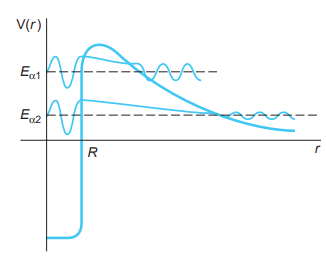
\includegraphics[scale=0.95]{AlphaBarrier}
\end{center}

\subsection*{Beta Decay}
Beta decay, on the other hand, is the emission of a beta particle, an electron or a positron. Energy spectrum is continuous in beta decay, the radiation is less ionizing and more penetrating than alphas. Three related types for beta decay: (1) the positron emission, called beta-plus, (2) the electron emission, called beta-minus, and (3) electron capture of one of its own electrons. Inn beta decay, sum of protons and neutrons, denoted as $A$, remains constant. Isobaric nuclides can turn into each other and emit, or absorb, an electron or positron via beta decay.\\

The fact that the beta particles do not have discrete spectrum suggests that another particle is emitted that shares the energy available, hence the occurrence of the the neutrino. Also, recall that neutron, proton and electron all have spin $1/2$. So, without an extra particle we cannot conserve the angular momentum either. The neutrino (little neutral one in Italian) was hypothesized by Pauli in 1930, and incorporated by Fermi into the theory of beta decay in 1933. The neutrino carries the energy, and momentum needed to obey conservation laws, and the neutrino has zero electric charge (charge is already conserved without it). Also, the neutrino is less massive than the electron (the beta particle takes nearly all the energy).\\

The neutrino was first observed in the lab by Cowan and Reines in 1957. Today we know that there are three neutrino flavors: electron neutrino, muon neutrino, and tau neutrino. The electron neutrino and anti-neutrino both participate in beta decay processes. The three types of beta decay can be mathematically generalized as the followings:
\begin{align*}
&_Z^AX \to {}_{Z+1}^AX' + e^- + \bar{\nu}_e \qquad\quad _Z^AX \to {}_{Z-1}^AX' + e^+ + \nu_e \quad\qquad _Z^AX+e^- \to {}_{Z-1}^A X' + \nu_e
\end{align*}
Notice that the electron is created in the beta decay process, neither electrons nor positrons exist inside the nucleus 
prior to the decay. This is analogous to how photons are created in atomic energy level transitions. Unlike the alpha decay, for which the nucleons are bound by the strong nuclear force, electrons and neutrinos in beta decay are not affected by the strong nuclear force and, since the neutron is uncharged, the electromagnetic interaction is not involved in beta decay. Therefore, we need to invoke a new force to explain the beta decay. The long half-lives of beta decay, compared to the characteristic nuclear time scale of the nucleus indicate that this new force is weaker than the strong nuclear force, hence the occurrence of the weak force.\\

\subsection*{Gamma Decay}
In gamma decay, a nucleus in an excited state decays to a lower energy state of the same isotope by the emission of a photon. $\gamma$-rays are very high energy photons. The process of gamma decay is an electromagnetic process, and this process creates the most penetrating radiation. The energy of the emitted photon ranges from several keV to about 8 MeV, corresponding to nuclei energy levels.  Gamma decay usually occurs after alpha or beta decay that leaves the nucleus in an excited state. The following figure compares the penetration power of the three types of decay:
\begin{center}
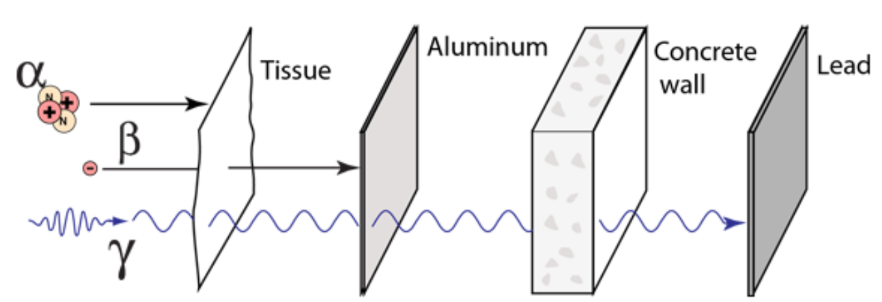
\includegraphics[scale=0.55]{penetratePower}
\end{center}

We have discussed different types of nuclear radioactive decay. 
\begin{enumerate}
\item \textbf{Alpha decay}. Binding force (nuclear strong force) counters the Coulomb repulsion of the charges in the nucleus. Tunneling process means that there is a small probability that charges will escape the nucleus. Emitted radiation of alpha particles, which are the He nucleus. The energy spectrum is discrete.
\item \textbf{Beta decay}. Emitted radiation is beta particles (electron, positron). The energy spectrum is continuous. Number of nucleons (A) is constant. New particle is introduced to explain the beta decay, which is the neutrino.
\item \textbf{Gamma decay} (emission of a photon). The gamma decay often occurs following an alpha or beta decay, since the daughter nucleus is frequently left in an excited state.
This gamma radiation is highly penetrating, but less ionizing then alphas or betas.
\end{enumerate}

\subsection{Fission}
Here we will discuss what happens when we hit the nucleus with a neutron.\\ In fact, typically there are three possible consequences:
\begin{enumerate}
\item The neutron can bounce off completely elastically. 
\item In some situations, the neutron bounce off inelastically, giving some of its energy to the nucleus. 
\item The neutron can also be absorbed by the nucleus, this leaves the nucleus in an excited state, causing it to decay back to the ground state via the emission of a gamma ray. 
\item The incident neutron splits the nucleus into two roughly equal parts, and such process is called the fission process. The amount of energy released per nucleus in this way is 10-100 million times more than a typical chemical reaction, due to the MeV scale of the binding energies.
\end{enumerate}

To figure out which of the four possibilities will happen in a given encounter of a neutron with nucleus, we first need to define the cross-section to represents the probability of a process to occur. The nuclear cross section is given in units of barns:
\begin{align*}
1\, \text{barn} = 10^{-24}\, cm^{-2}
\end{align*}
One can think of the cross
section for reactions as representing the size of the target presented by
the nucleus for that particular process. The cross section for a given type of neutron interaction turns out to depend very strongly on the neutron energy.\\

Here is an example of fission reaction:
\begin{align*}
^{235}U + n \to {}^{92}Kr + {}^{142}Ba+2n + 179.4\, MeV
\end{align*}
$179.4\, MeV$ is an incredible amount of energy, $10-100$ million times more than a typical chemical reaction because $MeV$ is a scale of the binding energies. Note that each fission reaction liberates additional
neutrons. These can instigate further reactions, leading to the possibility of a self-sustaining
nuclear reaction chain.\\

The neutrons liberated in fusion reactions have energies of order $1$ to a few MeV, so-called the fast neutrons. $^{235}U$ has a rather low fission cross section for neutrons of these energies, hence the incident neutrons are more likely to be scattered, causing them to reduce their energy still further to the point where they cannot fission the nucleus at all. Natural uranium is of $99.3\%$ $^{238}U$. On the other hand, $^{235}U$ has enormous fission cross section. Neutrons of any
energy cause it to fission, with the probability increasing dramatically at low energies. But natural uranium contains only $0.7\%$ $^{235}U$.\\

Hence, to build a nuclear power plant, we need lots of $^{235}U$, and some way to slow down the neutrons. The enrichment of $^{235}U$ is a very expensive process, and the moderation of neutrons, which is the process of slowing down neutrons by having them scatter off light maters, often involves heavy water $D_2O$ because it slows down the neutron but does not capture the neutron. \\

Some of the neutrons are not released in the fission process but by a later decay of the fission products. For example, we have:
\begin{align*}
^{87}Br \to {}^{87}Kr^* + e^- + \bar{\nu}
\end{align*}
while around $56\, s$ later, we have another process:
\begin{align*}
^{87}Kr^* \to {}^{86}Kr + n
\end{align*}
This is very important in allowing
one to control the reaction rate. Let the reproduction constant $k$ to be the average number of neutrons per fission that cause a subsequent fission, for a self-sustaining reaction we want $k=1$. Suppose further that the average time between fission generations is $0.001 \, s$, and suppose $k = 1.001$. The fission reaction rate $R$ after $N$ generations is given by:
\begin{align*}
R(N) = R(0)k^N 
\end{align*}
if $R$ is doubled, we want $R(N) = 2R(0) = R(0)k^N$, hence $N \approx 700$, and so the reaction rate doubles  in only $700 \cdot (0.001\, s) = 0.7\, s$, which is hard to be controlled mechanically. Now suppose that $0.65\%$ of the neutrons are delayed by $14 s$. Then the average time between generations is then given by:
\begin{align*}
t_{avg} = 0.9935(0.001\,s) + 0.0065(14\, s) = 0.092\, s
\end{align*} 
hence the rate-doubling time for $700$\, generations is $700(0.092\, s) = 64.4\, s$. The average time between generations is now around $100$ times longer than before, and resulting a much more controllable generation rate-doubling time.\\


On 2nd December, 1942, Enrico Fermi, and his team achieved the first nuclear chain reaction, Chicago Pile-1, under the Stagg Field, in Chicago.\\


In 26th April, 1986, the world's largest nuclear accident todate, the Chernobyl disaster, took place. About 300k-600k people were involved in the cleanup. The evacuation zone was initially 30 mi, and later expanded to 70 mi radius. Death toll is officially 30 people by Soviet, but people living close by received the equivalent of 37000 chest x-rays as internal radiation dose. The mortality of cleanup workers increased significantly, from 3.5 to 17.5 per 100k (until to 2012). The mortality of the general population in contaminated areas almost doubled, and there are increases in birth defects.\\



Breeder reactors generate their own plutonium fuel from non-fissile abundant $^{238}U$:
\begin{align*}
^{238}U + n \to {}^{239}U^* \to {}^{239}U +\gamma \qquad {}^{239}U\to{}^{239}Np +e^- +\bar{\nu}\qquad {}^{239}Np \to {}^{239}Pu + e^- + \bar{\nu}
\end{align*}

$^{239}Pu$ has a high neutron cross section across wide energy range, so no moderator needed.
$^{239}Pu$ has further advantage of yielding about 2.7 neutron per 1 fission for a neutron energy of 1 MeV. One of them can be used on neutron to sustain ration, the other can be used to create more fissile material.\\

Typical fast breeder can double its supply in about 7 to 10 years. But there are issues for using breeder reactors:
\begin{enumerate}[topsep=3pt,itemsep=-1ex,partopsep=1ex,parsep=1ex]
\item There are fewer delayed neutrons in this process, hence harder to control.
\item The temperature of this process is higher, hence need to be cooled with liquid Na, which reacts explosively with both air and water.
\item $^{239}Pu$ is the main fuel in nuclear weapons
\end{enumerate}
There are a few such reactors in operation in the world today.\\

\subsection{Fusion}
In fusion we move up the curve of binding energy from the low side, combining light nuclei into heavier ones. For example:
\begin{align*}
^2 H + ^3 H \to ^4He + n + 17.6\, MeV
\end{align*}
The considerable amount of energy released in this reaction, as well as the comparatively easy availability of hydrogen, make this a promising reaction for power generation. \\

But fusion reactors are a still long way from reality. The problem is that it takes kinetic energies on the order of 10 keV ($10^8$ Kelvin) to overcome the Coulomb repulsion of the two hydrogen nuclei. This is an area of active research. Such temperatures occur in the interiors of stars.\\

Up to now, we have discussed how we can extract energy from nuclear reactions: (1) Fission of heavy nuclei (beyond Fe), and (2) Fusion of light nuclei (up to Fe). Here we note that, in usual cases, fusion can give even more energy per reaction than fission, as indicated by the slope between regions of low and high nucleon numbers in the plot:
\begin{center}
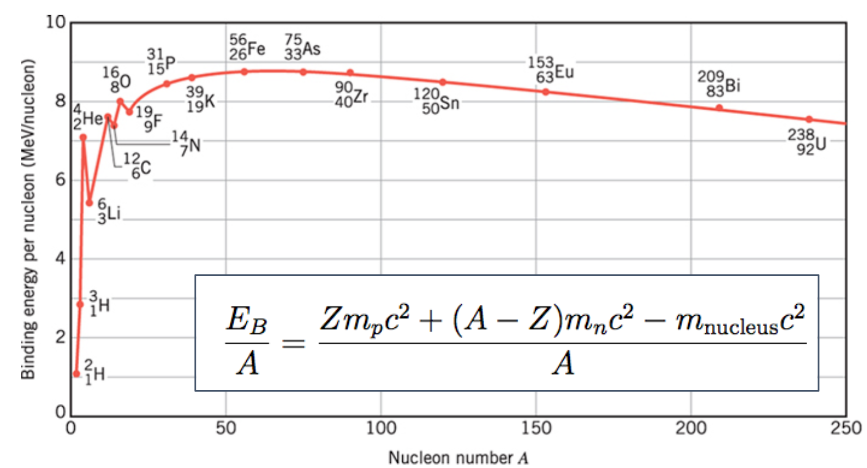
\includegraphics[scale=0.5]{FissionFusion}
\end{center}

\subsection{The life and death of stars}
Here we are going to discuss stars as examples of systems where nuclear reactions and the Pauli exclusion principle play key roles.  For any astronomical object, gravity tends to compress the mass. This gravitational collapse is halted once the material develops enough pressure to balance it. The greater the mass of the object, the greater the pressure required. The pressure comes in different ways:
\begin{enumerate}[topsep=3pt,itemsep=-1ex,partopsep=1ex,parsep=1ex]
\item Microscopic particles in movement (kinetic theory of gases)
\item Radiation pressure (photons carry momentum)
\item Degeneracy pressure (fermions, which obey the Pauli principle)
\end{enumerate}

The source of the energy to sustain the sun was a hot topic in the late 1800s. The debate involved big-wig names such as Lord Kelvin and Charles Darwin. The core of the argument is as follows. From the luminosity of the sun, one can estimate what would be its lifetime given different sources of energy. Chemical reactions have such a low yield that it would sustain the sun's present energy output for only 3000 years — that definitely cannot be right.
The gravitational energy converted into heat gives 30 million years — but that cannot be right either. Darwin had estimated 300 million years for natural selection to take place. The solution to this problem is nuclear reactions. \\

In terms of the formation of a star, molecular clouds in interstellar space start to collapse and rotate. Atom falls into the gravitational well, increases in the kinetic energy of the atoms means the temperature increases. Fusion ignites at about $1.5 \times 10^7\, K$, enough energy to overcome the electrostatic Coulomb barrier. Fusion of H to He is what sustains the sun, and all stars for most of their lives. The process occurs in chain reactions, such as the proton-proton cycle. The main reactions of the pp-cycle (yielding 26.7MeV each) are:
\begin{align*}
^1 H+{}^1 H \to {}^2 H +e^+ + \nu_e \qquad\quad ^2H + {}^1H \to {}^3He + \gamma \qquad\quad ^3He+{}^3He \to {}^4He + 2 {}^1He
\end{align*}
The net result is $4{}^1H \to {}^4He + 2e^+ + 2\nu_e + 2\gamma$.\\

There are also other possible reactions to turn $^1H$ to $^4He$, all with same $Q$ value. There are also alternative cycles, and their rates depend on the conditions of the star's interior. We cannot see through the photosphere of the sun, so how do we know our idea is correct? Messengers from inside the sun are neutrinos. The different reactions create different neutrino energy spectra, therefore providing a way  of determining  the relative contributions of each reaction and gaining further information about the composition and temperature of the core.\\

When the H supply is consumed, He-He fusion takes over, for example, we have $^4He + ^4He \to ^8 Be$, followed by $^8Be + ^4He \to ^{12}C$. Other reactions continue, moving up the binding energy curve and burn successively heavier elements until iron is produced. After that, even heavier elements are only produced by supernova and neutron star collision via neutron capture and beta decay, such as $^{58}Fe + n \to ^{59}Fe$ followed by $^{59}Fe\to ^{59}Co +e^- +\bar{\nu}_e$. Thus creating new elements, the two such processes are called the r-process and the s-process. They take place in supernovae and neutron star collisions.  \\

With new fuel cycle the star heats up more. Eventually the core starts to collapse but the outer layer expands outwards. Its luminosity stays approximately constant, hence intensity decreases, and radiation shifts to longer wavelengths. The star becomes first a red giant, then a red supergiant. The star possibly blowing off their outer layers into gaseous remnants that become visible as planetary nebulae. They do not collapse indefinitely, however, because they can be supported by electron degeneracy pressure. Recall that this arises because of the Pauli exclusion principle: the electrons
resist compression because of they must avoid being in the same state.\\

For relatively low mass stars, electron degeneracy pressure balances gravity after nuclear burning is over. The Fermi energy of nonrelativistic gas of free electrons is given by:
\begin{align*}
E_F = \frac{h^2}{2m_e}\left( \frac{3N_e}{8\pi V}\right)^{2/3}
\end{align*} 
There $V = 4\pi r^3/3$ is the volume of the star. On the other hand, the kinetic energy of the electrons is $3E_F /5$, the gravitational self-energy of the star is approximately $U = -(3/5)(GM^2/r)$. The thermal energy of the star is negligible here, in fact it slowly drops to zero as the star cools. So the total energy of the star is approximately:
\begin{align*}
E(r) = \frac{3}{5}N_e E_F - \frac{3}{5} \frac{GM^2}{r}
\end{align*}
Assume further that $M = Nm_n$, which says that the star consists of $N$ nucleons, and also assume $N_e = N/2$, which says that there are half as many electrons as there are protons and neutrons. To find the equilibrium radius, one can set $dE/dr = 0$ and obtain the following result:
\begin{align*}
R = \frac{3^{4/3}\pi^{2/3}}{8}\frac{\hbar^2}{Gm_em_n^2}N^{-1/3} = \frac{3^{4/3}\pi^{2/3}}{8}\frac{\hbar^2}{Gm_em_n^{5/3}M^{1/3}}
\end{align*}
This expression gives a radius of about 7000 km for a 1 solar mass star, or about the size of the earth. This also implies an incredible density, around $10^9\, g/cm^3$ for $1M_{\odot}$. The more massive the star, the smaller the radius, but there is a Chandrasekhar limit of  $1.4M_{\odot}$. Star having a mass more that the Chandrasekhar limit does not form a white dwarf, but instead continues to
collapse, blows off its gaseous envelope in a supernova explosion, and becomes a neutron star. \\

Electron degeneracy pressure cannot support any mass, because $E_F$ increases with  $E_F \propto M^{4/3}$. Since the star is not at zero temperature, there's high-energy tail to Fermi-Dirac distribution that gives electrons energies greater than $E_F$, which allows for inverse beta decay $e^- + p \to n + \nu_e$. If one electron is removed through the beta decay, the star collapses a bit, and hence rate of inverse beta decay increases, so soon all electrons are eaten, and we have only neutron left. Neutrons are also fermions with their own degeneracy pressure, hence neutron star can form. The typical radii for neutron star is around 10 km, and density around  $1.2 \times 10^{14} g/cm^3$. For neutron stars, the neutron degeneracy pressure applies and one can compute the radius of the star:
\begin{align*}
R = \frac{3^{4/3}\pi^{2/3}}{2^{4/3}} \frac{\hbar^2}{Gm_n^3}N^{-1/3}
\end{align*}
Neutron stars are even more compact than white dwarfs.\\


Neutron stars drew little interest until the late 1967 when pulsars were
discovered by Jocelyn Bell Burnell. Pulsars emit extremely regular bursts of radio waves with periods ranging from a few milliseconds to about a second or so. The bursts of radio signals were through to be sent by Aliens at the beginning, but soon after, it was discovered that the origin of the signal was due to the spinning of the neutron stars. The sun rotates on its axis about once a month, but if you compress it down to neutron star densities you would indeed find a rotation period of about a second. So the observed periods of pulsars make sense. It is thought
that the radio pulses are caused by a lighthouse beam of radiation that is produced by the very strong magnetic fields in the vicinity of the neutron star, in which protons and electrons are accelerated. We see the radio blip when the beam crosses the earth. \\


There exist also neutron star binaries, which are excellent probe to test General Relativity.\\

Event neutron degeneracy cannot hold up arbitrarily high mass. At about $2M_{\odot}$ to $3M_{\odot}$, we begin to have collapse into a singularity, a black hole. About one year after Einstein's GR paper, Schwarzschild solved the equations for symmetric spherical mass distribution, he found that, compared to a reference clock far away from any gravitational fields, the clock will tick at a rate given by:
\begin{align*}
\Delta t = \Delta t_0 \sqrt{1-\frac{2GM}{rc^2}}
\end{align*}
where $\Delta t_0$ is the rate of the reference clock. To the distant observer, the clock in the gravitational field appears to stop ticking. Any radiation
emitted from this radius would be redshifted to zero frequency. So nothing can escape from this
radius, which we call the event horizon. Thus the name black hole. Black hole is incredible compact, the Schwarzchild radius for the Sun is only around $3\, km$, and $1\, cm$ for the Earth. There is a supermassive hole at the center of the galaxy.\\




\newpage
\section{The Standard Model}
A proper treatment of  Quantum Mechanics must also include Special Relativity. The Schrodinger Equation cannot accomplish that, as it fails when we consider systems approaching the speed of light.
Pondering the problem, Dirac realized that the wave function must have multiple components (not just one as in Schrodinger equation).
Dirac's formulation accounts for special relativity in the context of quantum mechanics. It describes the behavior of spin that cannot be described classically. It also predicted anti-particles and laid the foundation of Quantum Field Theory. All known particle have anti-particles with identical properties but opposite charge.\\

We have four fundamental forces:
\begin{enumerate}
\item Gravitational force, governed by:
\begin{align*}
F_g = \frac{Gm_1m_2}{r^2}
\end{align*}
Note, however, that gravity is completely negligible on subatomic distance scales.
\item The electromagnetic field, governed by:
\begin{align*}
F_e = \frac{kq_1q_2}{r^2}
\end{align*}
\item The strong nuclear force, which operates at short distance, and has strength $10$ to $100$ times that of the electromagnetic force. The strong force does not affect all particles, the particles that are affected by the strong force are said to carry color. The gluon $g$, which mediates the strong force in the same way that the photon mediates
the electromagnetic force, carries color charge.
\item The weak nuclear force, which is also a short-range force, with a range not too different from the electromagnetic force. All particles feel the force, and the quantity analogous to electric charge associated to weak nuclear force is called the flavor. The force is carried by $W^\pm$ and $Z^0$.
\end{enumerate}

Our modern viewpoint is that all forces are caused by local interactions. A very useful way to picture this is via Feynman diagrams. We view all forces as being caused by the exchange of particles that carry or mediate the force. The mass of the exchange particle explains the range of the force. Photons and gravitions are
massless, hence their range is infinites. Gluons and the $W$, $Z$ bosons are massive and therefore are only of short range. Basic elements of a Feynman diagram includes:
\begin{enumerate}[topsep=3pt,itemsep=-1ex,partopsep=1ex,parsep=1ex]
\item particles as represented by solid arrows, the arrows are not trajectories of the particles in space.
\item interaction points, represented by the the primitive vertex. A given particle enter, emits or absorbs another particle, and then exits the interaction point.
\item mediators, as represented by wavy lines, or some other type of line.
\item anti-particles as represented by arrows pointing backwards in time
\item time and space axes are often omitted
\end{enumerate}


\subsection{Quarks and Leptons}
Subatomic particles are generally classified as Leptons and Hadrons:
\begin{enumerate}
\item Leptons are particles that do not feel the strong force, or colorless. The three generations of leptons are $e$, $\mu$, and $\tau$, with progressively increasing mass. All leptons have spin-half. Electron, muon, and tatauuon all have their own neutrino $\nu_e$, $\nu_\mu$, and $\nu_\tau$. Because the muon and the tau are heavy, they are unstable and decay quickly via the weak interaction into lighter particles. As far as anyone has been able to tell, these leptons are fundamental particles, with no
indication of internal structure.
\item Hadrons are particles, like the proton and neutron, that do feel the strong interaction force. Hadrons are further subdivided into Baryons and Mesons. Baryons are fermions that have spin-half, such as proton and neutron. Mesons are bosons that have integer spin, such as $\pi, K, \rho, w, J/\psi$.
\end{enumerate}


The $K^\pm$ mesons have a lifetime of about $10^{-8}$ seconds, which sounds short but is much longer than we would
expect them to live if they decayed via the strong interaction. This strange property of $K$ mesons led physicists to postulate that they possessed a new quantum number, strangeness, that
was conserved by the strong, and electromagnetic, interactions but not by the weak interaction. So the $K$ mesons can only decay via the weak interaction.  Later, new mesons were discovered that had unusually long lifetimes but whose decays did not appear to violate the conservation of strangeness. Such mesons were called charmed, and were hypothesized to possess a new quantum number called charm. Again, charm could only be changed by the weak interaction. This process repeated itself in the late 1970s with the discovery
of yet additional mesons that possess a quantum number known as bottomness.\\

This profusion of particles and bizarre quantum numbers sounds contrary to the particle physicist's desire for reductionist simplicity. Fortunately, a very simple picture explains all of this, and a wealth of other data as well. This picture is known as the quark model. Protons and Neutrons are made of quarks. Quarks are strongly interacting particles with spin half and factional charge, $2/3$ for up quarks and $-1/3$ for down quarks. Quarks always bound to produce an integer charge, it is impossible to observe an individual quark.\\

In the quark model, we view mesons and baryons, in other words, all the strongly-interacting particles, as being bound states of quarks. A baryon is a bound state of three quarks, mesons are bound states of a quark and an antiquark. Quarks include up and down quarks, strange and charm quarks, and top and bottom quarks.  The strangeness quantum number of a particle is simply the number of strange quarks it contains. Likewise for charm, and bottom. The top quark is so heavy and unstable that it does not live long enough to form bound states. We interpret these conservation laws as saying that the strong interaction cannot change
one type flavor of quark into another. Only the weak interaction can do that.\\

The standard model generally consists of the organization of matter particles into three generations of quarks and leptons,  dynamical rules, analogous to Maxwell's equations, that describe how these particles interact with each other via the force carriers gauge bosons, and an additional, spin-0 particle called the Higgs boson that generates structure of vacuum and leads to masses of particles via the Higgs mechanism. The dynamics rules are expressed in the language of a particular kind of relativistic quantum field theory known as gauge theories. The role of Higgs boson is to endow all particles with mass through their interactions with the Higgs. When it does this to the $W$ and the $Z$, it
breaks a symmetry that exists between the weak and electromagnetic interactions. The discovery of the Higgs boson, in 2012, at the Large Hadron Collider at CERN, represents a crowning achievement of the Standard Model.\\

The key postulate of the Higgs mechanism is a new force field, called the Higgs field, which has an average value in the vacuum that became non-zero as the early universe cooled. Photon is non-interacting with the Higgs field, while other particles, such as electrons, top quarks, and so on, will interact with the field and slow down.\\

The standard model predicts physical phenomena at the order of ten parts in a billion, and it  has been tested with the world's largest experiments. In general, interactions are long or short range, in the macroscopic world the long ranges govern, the short range in the microscopic world. The production and decay of particles is governed by conservation laws and kinematics. The Standard Model is very powerful and can explain all the phenomena in the microword of particles in a simple and unified way, at least in principle. \\

\subsection{Neutrinos}
Neutrino is another success story of experimental particle physics. We have seen one example, a big success case, the discovery of the Higgs boson at the LHC. Neutrinos are so-called the ghost particles because they interact very rarely, but when they do interact, they create a lepton, which is typically a electron or a muon. \\

The Sun is powered by nuclear reactions producing a very large flux of neutrinos. Number of experiments saw a deficit of neutrinos compared to experimental prediction, and that leads to the Solar Neutrino Problem. \\

Ray Davis searched for solar neutrinos in the Homestake Mine in the late 1960s by performing an experiment. He used at tank with 100,000 gallons of tetrachloroethylene, in attempt to count neutrinos, subatomic particles
produced in fusion reactions inside stars.  The ${}^{37}Ar$ atoms are extracted by bubbling helium gas through the tank every few weeks, and the number of ${}^{37}Ar$ decays are counted in a low background environment:
\begin{align*}
^{37}Cl + \nu_e \to {}^{37} Ar + e^-
\end{align*}
However, the neutrinos detected were only about a third of those expected from the best models of the Sun's interior. Since we have accurate measurements of the amount of energy released by the Sun, a factor of three changes in the rate of the main production reactions is hard to explain.\\

One explanation, first predicted by Bruno Pontecorvo, is that neutrinos can change their flavor, that is, electron neutrino can become a muon neutrino and vice versa. Neutrinos other than electron neutrinos couldn't be detected by the experiment and this would explain the apparent lack of neutrinos since we do not measure
the total neutron flux. Neutrinos oscillate only over long distances, hence seems conserved at local experiments. In the late 1990s finally, the Sudbury Neutrino Observatory (SNO) and the Super Kamiokande neutrino detector in Japan found evidence for this neutrino oscillation, and their combination allowed to deduce individual components and the total flux of solar neutrinos. The result agrees well with the Bahcall calculation of solar neutrino flux. 










\newpage
\section{General Relativity}
In the discussion of the standard model, we purposefully left out gravity. Gravity is the weakest of the four fundamental forces. Einstein's theory of gravity, General Relativity (GR), is remarkably successful in describing the observations. The equivalence principle is the bedrock of GR, which states that inertial mass of and object is equal to its gravitational mass:
\begin{align*}
F = ma = \frac{GMm}{r^2}
\end{align*}
Einstein, while working in a patent office in Bern, Switzerland: ``Suddenly a thought struck me. If a man falls freely, he would not feel his weight. This simple thought experiment, led me to the theory of gravity." He recognized a deep relationship between systems affected by gravity and ones that are accelerating. No experiment can tell the difference between the fictitious force produced by uniform acceleration and the acceleration produced by a uniform gravitational field.\\

Consequence of the equivalence principle is that photons are redshifted when climbing out of a gravitational potential well. Consider doing an experiment with a beam of light in an elevator. One places a light source at the bottom of the elevator, a distance $h$ below a detector which we place at the top. Suppose the elevator is accelerating upward uniformly at $10\, m/s^2$ in free space, and for simplicity we suppose that the velocity of the elevator at this instant is much less than the speed of light. Let the source emit a pulse of light with frequency $f$ at $t = 0$. In the time $t = h/c$ that the light takes to reach the detector,
the detector acquires a velocity $ v = gt = gh/c$. Thus the detector sees the light redshifted to a frequency $f'$, where for small values of $v/c$, we have:
\begin{align*}
f' = f\left( 1-\frac{v}{c}\right) = f\left( 1 - \frac{gh}{c}\right)
\end{align*}
According to the principle of equivalence, this situation should be exactly the same if the elevator
were at rest on the surface of the earth. In that case, note that the quantity $gh$ that appears here is simply the difference in the gravitational potential between the source and the detector. So general relativity makes the following prediction: \textit{Light propagating out of a gravitational potential well is redshifted; light propagating into a gravitational well is blueshifted.}\\

If the gravitational field through which the light passes is not constant, say, for example, we have a photon emerging from near the horizon of a black hole to be observed by an observer far from any gravitational fields, then we need to replace constant $g$ with $GM/r$, and replace $h$ with $dr$, and integrate. The result is given by the following:
\begin{align*}
\frac{f'}{f} = 1\pm \frac{GM}{c^2 R}
\end{align*}
where $R$ is the radius from which the light emerged.\\


Another consequence of GR is that clocks will run slower in the presence of a gravitational field than otherwise — if the frequency goes down, due to gravitational redshift, then the time between ticks of the clock will increase. An example includes the GPS satellite signals, which orbit the earth at 14000 km every 12 hours. They must be synchronized taking into account two effects: (1) Special relativity time dilation, which slows down by a factor of $5\cdot 10^{-11}$, and (2) the General relativity gravitational redshift, which speed up by a factor of $-4.8\cdot10^{-10}$. Note that the GR effect here is one order of magnitude larger than the special relativity effect.\\


In place of Newton's action at a distance, Einstein's theory says that matter and energy cause spacetime to curve: think of a bowling ball placed on a rubber sheet. This spacetime curvature, in turn, means that particles no longer follow straight paths. The parabolic trajectory of a baseball,
in the language of GR, is actually a straight path through curved spacetime.  A profound consequence of general relativity is that light itself can be bent by gravity. It is better
to say that the curved spacetime produced by a massive object is a geometrical fact of life that
affects the motion of everything, light included. This phenomenon provided the first key test of general relativity, a test suggested by Einstein himself. Stars near the rim of the sun should
appear slightly displaced relative to their position when the sun is far away; the deflection angle turns out to be given by the following:
\begin{align*}
\alpha = \frac{2GM}{c^2 R}
\end{align*}
where $R$ is the radius of the sun. One can set up an experiment to verify the effects of general relativity. The observation of stars directly behind the Sun is made possible during eclipse. Such experiment was performed on May 29th 1919, the eclipse that made Einstein famous. \\

In general relativity, it is not really correct to say that the light is bent. Rather, the light is following a straight line, but in a curved spacetime. This effect is also observed in the phenomenon known as gravitational lensing, in which the light from distant quasars or galaxies can be distored, sometimes quite spectacularly, by massive foreground objects such as galaxies or clusters of galaxies. This fact is used by astronomers to infer the mass of galaxies and other objects that cannot be directly seen.\\

Gravitational waves is analogous to EM waves, with some important differences that the lowest order of emission of gravitation waves is quadrupole instead of dipole for EM waves, and gravitational wave is due to the oscillation of tensor field, instead of vector fields for EM waves. \\




On September 14 2015, the LIGO detectors at Hanford and Livingston observed a binary black hole merger event, called GW150914, that was the beginning of the era of astronomy with gravitational waves. The discovery was awarded the Nobel prize in 2017. On the other hand, GW170817 was the fist binary neutron stars merger ever detected. Electromagnetic signature of the merger was also captured, which was the first multi-messenger event. Many collaborating teams involved, including the group of UM Professors Reiles and  Soares-Santos.\\


\newpage
\section{Cosmology}
Modern physics has been a great success in explaining phenomena at the smallest and largest scales, from elementary particles, to stars, and the universe. In the following we will discuss how general relativity and the standard model allows us to build a picture of the universe's origin and evolution, and how our most successful theories still leave much about the universe to be explained, including the dominant components of the present day universe, the dark matter, and the dark energy.\\

In the classical, Newtonian, model of the universe we have a infinite static universe in which objects move in accordance to Newton's law of gravitation. Moreover, the cosmological principle states that the universe, on average is isotropic, which means that we have same features no matter what direction you look; The universe on average is also homogeneous, which means that we have same features no matter where you are located in the universe. However, there is problem with this picture, that it fails to explain the most basic observation that the night sky is dark. This is known as Olber's paradox.\\

We now know that universe is billions of years old and filled with galaxies containing billions of stars each. Until the 1920s however, it was unclear that the observed nebulae were in fact outside of the Galaxy. Edwin Hubble made a breakthrough by measuring the spectrum of distant galaxies and discovering that they were receding from us.\\

Observational data reveals that there is a linear relationship between the distance of star from us and the recession velocity of the stars:
\begin{align*}
v = H_0 d \tag{Hubble's Law}
\end{align*}
with the constant:
\begin{align*}
H_0 = 50 \sim 100 \ \frac{km/s}{Mpc}
\end{align*}
This result can be interpreted as the universe expanding. \\

The challenge is measuring the distances of the stars from us. An analogy is how one can make a map of a city based solely on photographs of its skyline. The method of standard candles uses a source (that exists in all galaxies, if possible) that has a known luminosity and then use the inverse square law to calculate the distance of that galaxies.  \\

For stars closed enough, one can make use of the periodic brightness variation of $\delta$-Cephei and its corresponding period-luminosity as a candidate of the standard candles. For galaxies that are far away, one can make use of the Type Ia Supernova, in which the aging companion star starts swelling, spilling gas onto the white dwarf, and the white dwarf's mass increases until it reaches a critical mass and explodes, from which we can measure the luminosity of the galaxy. For the Type Ia Supernova,  the lightcurve shape (brightness over time) is related to the intrinsic brightness of the Type Ia Supernova explosion. 
They provide relative distances that  can be calibrated in nearby galaxies where Cepheids can be observed. Note that Cepheids themselves also have to be calibrated to get to absolute distances. This procedure is known as distance ladder.\\

There are other standards for distance measurements in cosmology. The standard candles are objects of known brightness that we have discussed above. The standard rulers are objects of known angular size, such as baryon acoustic oscillations from the CMB. The standard sirens are objects of known gravitational wave signal, such as binary neutron stars and black hole mergers.\\

Recall that matter tells space how to curve:
\begin{align*}
G_{\mu \nu} = 8\pi G T_{\mu \nu}
\end{align*}
where $G_{\mu\nu}$ is the Einstein Tensor, which tells the curvature of space-time of the expanding Universe, and $T_{\mu\nu}$ is the Stress–Energy–Momentum Tensor, which tells all matter and energy in the Universe. 

The expansion is explained as an overall expansion of the geometry, an analogy is a rising loaf of bread. Moreover, the theory allows us to think of the universe as finite without having trouble with an undefined outside, an  analogy is the surface of a sphere which is a finite surface sans boundary. Einstein was horrified by this theory, he believed in a static universe, and he  thought there is something wrong with his theory. Hence he added the cosmological constant $\Lambda$ in the equation:
\begin{align*}
G_{\mu\nu} + \Lambda g_{\mu \nu} = 8\pi G T_{\mu \nu}
\end{align*}
where $\Lambda$ is an intrinsic energy density of the vacuum, and the term $ \Lambda g_{\mu \nu}$ provides attractive force to counteract the expansion. When Hubble discovered the expansion of the Universe Einstein called this ``\textit{the greatest blunder mistake of my life}". Today we know that the expansion is actually accelerating. Note that by flipping the sign of the cosmological term Einstein's equation features a built-in  term to account for that acceleration, and that is related to the idea of Dark Energy.\\


It is useful to describe the expanding of the universe using a scale factor $R(t)$, which is normalized such that we have today $R(t_0) = 1$. The exact behavior of $R(t)$ depends on the matter-energy-content of the universe. $R(t)$ gives us clues about beginning and the final fate of the universe. The rate of expansion of the universe is given by the first derivative of the scale factor:
\begin{align*}
H(t) = \frac{dR/dt}{R}
\end{align*}
The Hubble constant $H_0$ is the value of $H(t)$ at present.
\begin{center}
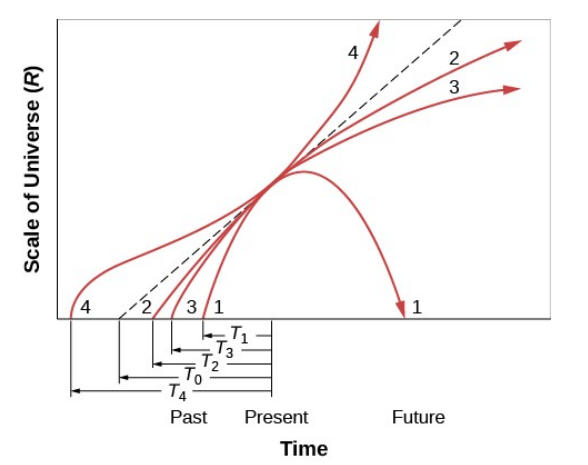
\includegraphics[scale=0.8]{scaleFactor}
\end{center}

The matter-energy-density $\rho$ will decide if the universe will expand forever, slow down and stop, or will recollapse. The density at which expansion just halts is denoted as $\rho_c$, given by around $10$ H-atoms per cubic meter, and the density parameter is defined by:
\begin{align*}
\Omega = \frac{\rho}{\rho_c}
\end{align*}
The presently best measured value of $\Omega$ from CMB is given by $\Omega = 1.082 \pm 0.032$, which means that the universe is balanced on a knife's edge. 
\begin{center}
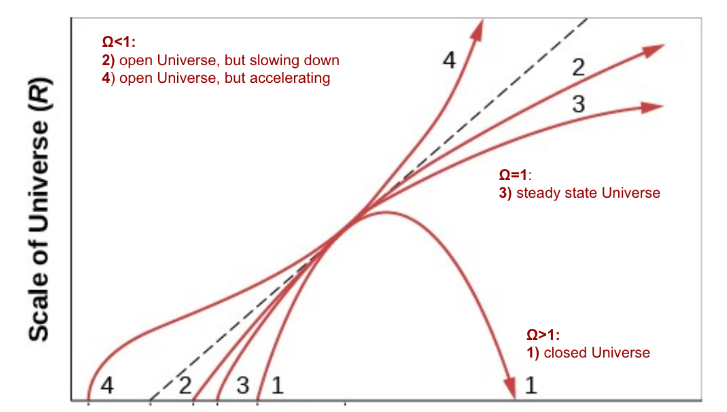
\includegraphics[scale=0.65]{Omega.png}
\end{center}


\subsection{Dark Matter}
It took a few hundred years, with the discovery of the Higgs boson the Standard Model has been completed. However, this is just the tip of the iceberg. Based on the Planck measurement we can deduce that the Universe contains 4.9$\%$ (baryonic) ordinary matter, 26.8$\%$ dark matter and 68.3$\%$ dark
energy. According to the measure of visible mass, single galaxies were moving too fast for the cluster to remain bound together. Visually, many spiral galaxies have a bright central bulge, and if the mass follows the light, then we expect most of the galaxy's mass to be concentrated near the center as well. This idea we
can test by observing the velocities of stars orbiting the center. We can do this by measuring the difference in the redshift from one side of the galaxy to another, as a function of distance from the center. This measurement is known as a rotation curve. If most of the mass lies near the center, we expect the motion of these stars to be described by Kepler's 3rd law:
\begin{align*}
T^2 = \frac{4\pi^2r^3}{GM}
\end{align*}
where $T$ is the orbital period of the star around the galactic center, $r$ is the radius of the orbit,
and $M$ is the mass that lies inside radius $r$. Since $T$ = $2\pi r/v$, we expect $v=\sqrt{GM/r}$. But instead we see velocities that are approximately constant with radius. This result implies that the mass within a given radius is increasing linearly. Since the light output from galaxies does not increase radially in this way, it implies there is a much larger, unseen mass present, the dark matter.\\

We can infer the motion and amount of dark matter from the motion of stars around us. The GAIA satellite is creating a 3D map of our Galaxy using 1.7 billion stars.\\

Local dark matter density is around $0.3 GeV/cm^3$. The volume of Earth is around $10^{27} cm^3$, hence there is only
about $0.5 - 1$ kg of dark matter on Earth, which is just a few cups of
coffee.\\

Dark matter is very weakly interacting with regular matter, hence they are ghost-like particles. The mass of all of the dark matter in the solar system is about $10^{17}\, kg$, about the mass of a small moon. \\

It turns out we know pretty well how the present universe came into existence, we can measure something called Baryon acoustic oscillations. The cosmic microwave background is light from the beginning of the universe, when matter came into existence, that traveled 13 billion years to reach us. During its long journey it red shifted it into the microwave regime. Waves in the first matter created ripples in the CMB which allow us to estimate the composition of the Universe. These ripples, regions of higher gravity, collapse to dark matter halos that were the progenitor or our galaxies. We can also see dark matter using the gravitational lensing method, that is light is bent by gravitational potential, and hence one will get multiple images of the same object. \\

In summary, based on cosmological observations, we know that dark matter causes the outer parts of galaxies rotate faster than expected from their starlight. Dark matter confines the hot X-ray gas that would otherwise evaporate from a galaxy cluster. Dark matter is also responsible for the scale of $10^{-5}$ of temperature fluctuations in the maps of the CMB. Furthermore, Dark matter's gravity was progenitor of today's galaxy cluster and super-clusters.\\

We have three ways to detect dark matter. 
\begin{enumerate}
\item Indirect search for dark matter where we know it exists in the Universe. Look at places where we expect particularly large amounts, such as the center of the Galaxy, Galaxies which are dark matter dominated, and objects with massive gravity like the sun. Indirect searches assume that dark matter interacts with itself and that in this interaction high energy particles are produced. These particles then decay
further via a process called hadronization into gamma-rays, cosmic-rays, neutrinos, anti-matter etc. These particles might appear as an excess over the expected cosmic ray flux. There are indication in the cups profile of galaxies that DM self-annihilates. The Galactic Center Excess is a surplus of events
in the gamma-rays after subtraction of all known foregrounds. Unfortunately the modelling of
backgrounds (foregrounds) in the Galactic Center that is very active is difficult and the debate
if this is a real DM signal or a poorly understand background, for example pulsars just below
their detection threshold, is an ongoing process.
\item If the mass of DM is within the energy range accessible at particle accelerators such as the LHC,
then we would be able to produce DM directly in the laboratory. While there is no guarantee that
DM is produced in present collider. A dark matter particle produced in a high energy
collision escapes the detector undetected. The key to find them lays in the fact that the particles that we collide themselves can emit a high energy visible particle such as a photon or a jet. If then in addition a DM particle is produced, independent of us knowing details of this new physics process, then the DM particle has to recoil from this known, visible particle. This is the so called mono-X signature, whereas X could be a whole range of known particles such as $\gamma,W,Z$ or the Higgs boson.
\item Direct detection refers to the detection of a cosmic DM particle by scattering off a nucleus that
passes through an detector while Earth is passing through the galactic DM halo on its orbit.
While most DM particles would not interact with any matter, sometimes - although exceedingly
rarely - there is still an interaction with a few atoms in the detector. This transfers momentum
that then manifests itself either as light, heat or charge produced in the target material. In
contrast to collider, the velocity of the DM particles entering Earth from outer space is relatively
slow, the velocity of Earth's orbit relative to the DM halo is just about $v \approx 10^{-3}c$. Assuming
that dark matter is made of particles at the electroweak scale then their kinetic energy, and
hence the maximal energy deposited in the detector, is just at the order of a few keV. These
are energies comparable or even lower as many natural backgrounds, for example comic rays or
natural radioactivity. In addition such events are expected only a few times per year in a given
detector, far fewer than background processes. The task of direct detection is therefore to build
the most sensitive detectors with the least amount of backgrounds. Therefore detectors are placed
deep underground to shield from cosmic rays and external backgrounds and are using the most radiopure material. Backgrounds are then further reduced by using passive and active radiation.
\end{enumerate}

\subsection{Dark Energy}
Previously, we discussed how our modern physics framework allows us to build a picture of the universe's origin and evolution. However, much about the universe remains to be explained, including major components of the present day universe. Dark Matter constitutes 25$\%$ of the total content of the present Universe. There is an abundance of evidence for dark matter. Examples include galaxy rotation curves, gravitational lensing, and galaxy clusters, We do not know what dark matter is made of, but we know that it interacts gravitationally like normal matter. So, it will tend to clump together, and those clumps will tend to grow as the universe evolves. Dark energy, however, is a totally different story. \\

In 1998, two competing groups published independent measurements of the cosmic expansion history showing evidence that the rate of expansion was accelerating. Such discovery of accelerated cosmic expansion leads to 2011 Nobel Prize. The expectation, assuming general relativity theory and traditional matter filling the universe, was that the expansion would be decelerating after the initial push from the big
bang. Within the standard cosmological framework, this acceleration of expansion must be due to a substance that behaves as if it has negative pressure, and it requires some new form of energy, called dark energy. \\


Cosmological redshift results from recession velocity. Radio waves stretched, and galaxy moves away as universe expands. Redshift is related to the scale factor, which is a function of time. Therefore, the distance-redshift relation maps the cosmic expansion history. \\

 Today we know that approximately 70$\%$ of the universe is dark energy. Einstein's cosmological constant $\Lambda$ fits the bill somewhat. An understanding of its physical nature is lacking, though. Dark Energy is clearly beyond the standard model, we are interested in what it is made of, whether it result from a 5th fundamental force, and whether it is really a constant, or just slow evolving.\\


Because dark energy affects the universe only on cosmic scales, experiments must rely on astrophysical observables to study its nature.\\

The Dark Energy Survey (DES) was the first sky survey designed to shed light onto the dark energy problem combining distance and growth of structure measurements, with more than 500 million galaxies, and more than 4000 supernovae. Initial results are exciting. Tension between different observables may be a clue to non-Lambda dark energy. The dark energy camera (DECam) is installed on the 4-meter Blanco Telescope in Chile since 2012. The Blanco/DECam system was the most powerful telescope/camera system of its time, with wide field of view, 
large aperture, and very sensitive CCDs. \\

DESI is installed on the Mayall 4-meter telescope in Arizona, collecting spectroscopic information for over 35 million galaxies. With a smaller number of galaxies, but much more detailed information relative to DES, DESI will yield precision measurements of the cosmic expansion history. It took only 5 months for DESI's spectroscopic dataset to surpass all other — existing and previous — telescopes combined.

The Vera Rubin Observatory's Legacy Survey of Space and Time (LSST) camera is a brad new camera that will provide a movie of the sky, spanning a 10 year timescale, with images of over 37 billion galaxies. LSST will do in one month, what DES did in 6 years. Rubin LSST will be the next leap in dark energy research. Deep, Fast, and Wide: next-generation imaging survey.\\

\subsection{A Brief History of the Universe}
As we discussed previously, one of the greatest achievements of modern physics is the ability to explain phenomena ranging from the smallest to the largest scales. 
And there is no other field that benefited more from this success than cosmology. \\

The Big Bang occurs as the beginning of time itself, at $t=0$. The questions are: What caused this explosion? Was there anything beforehand? Right now we cannot answer these questions, and it is possible that we may never know. Known laws only take us so far. However, there are clear evidences for the Big Bang:
\begin{enumerate}
\item The universe is expanding, as reflected by the Hubble's Law
\item  The existence of the cosmic microwave background radiation with the predicted temperature and blackbody distribution. The Big Bang theory predicts that the early universe was a very hot place and that as it expands,
the gas within it cools. The radiation left over from this early stage of the Universe has been redshifted to become the CMB.
\item  The abundance of the light elements as discussed below. 
\end{enumerate}

At the earliest of times just after $t=0$, the density of the universe is so high that gravity is as strong as the other three fundamental forces.  At this point, we say that all the forces were indistinguishable and unified. To analyze the quantum nature of space time we need a quantum theory of gravity to describe these conditions, but such a theory is lacking. We can, however, estimate the timescale that characterizes this situation, called the Planck time, using the fundamental constants: 
\begin{align*}
t_{Pl} = \sqrt{\frac{\hbar G}{c^5}} = 5.4\cdot 10^{-44}\, s
\end{align*}
Inflation is a brief period of exponential expansion in the early universe starting at around $t=10^{35}\,s$ and ending at around $t= 10^{-32}\,s$. This expansion is thought to result from a phase transition that occurs when the strong force
becomes physically distinct from the electromagnetic and weak forces, and this period of time is needed to solve two problems with the standard big bang theory: (1)The Horizon problem, and (2) The Flatness problem.\\

The Horizon problem is observed in the uniform CMB maps. It can be solved with inflation, which makes the causally connected regions expand quickly early on, when the primordial gas is in thermal equilibrium. The region of our visible universe was part of a single, causally connected region before inflation, so
it had a common temperature. The radiation pattern was preserved when inflation took
over, so a single uniform temperature characterizes our visible region even after inflation stops and the various causally disconnected regions can no longer talk to each other. At the time of decoupling, at which radiation looked at the time electrons and protons combined to form stable atoms, there are around $10^5$ 
causally disconnected domains.\\

For the flatness problem. It is an observational fact that the universe is flat or nearly so, the flatness of the universe is frequently characterized by $\Omega =  \rho / \rho_c$. If $\Omega = 1$, the universe will expand forever, asymptotically slowing to zero. If the Universe started off far from critical $\Omega = 1$, then it would have either quickly collapsed or it would have expanded so quickly that it would have passed through the nucleosynthesis so fast that we would not be here. The only way for the Universe to have lasted this long and have the observed abundances of elements is if the Universe started off very close to critical. Typically, we would have expected the universe to have recollapsed by now, or to have expanded away to the point where little else besides our own galaxy is visible. Such extraordinary fine tunings of fundamental parameters generally do not occur by accident. Inflation solves the flatness problem by postulating that the exponential expansion drove the universe to be much larger than the visible portion we can observe today. Just as the earth looks flat because we are small compared to the curvature of the earth, the universe looks flat because we can only see a small portion of it.\\

At $t=10^{-6}\, s$, we start to have formation of nuclear matter. At this point, quarks can build into protons, neutrons, and so on. Roughly equal numbers of each particle type are produced at this time. In particular, there are about as many proton as neutron because of the reactions:
\begin{align*}
n + \nu_e \leftrightarrow p+e^- \qquad\qquad\qquad n+e^+ \leftrightarrow p+\bar{\nu}_e
\end{align*}
The two reactions occur in equilibrium. As the temperature falls in the following eras, the conversion of (lighter)
protons into (heavier) neutrons will become disfavored.\\

At $t= 10^{-2}\, s$, the energy associated to temperature falls to about 13 MeV. Below the energy threshold for producing pions and muons. The ones that were produced at earlier times decay into electrons, positrons, and neutrinos.
Nucleons and anti-nucleons can no longer be produced either.
Most of the nucleons and their anti-antimatter counterparts annihilate. It is a miracle, in fact, that matter and antimatter do not exactly cancel each other and leave a universe consisting entirely of photons and neutrinos. Asymmetry of only a part per billion.\\

At $t=1\,s$, we have neutrino decoupling. Temperature falls below the threshold (1.7 MeV) for the neutrino capture reaction $
n + \nu_e \to p+e^-$. There are no other significant reactions they can have,
and so they decouple and do not interact anymore. Neutrinos now are decoupled from the primordial plasma and travel freely. The result is a cosmic neutrino background (analogous to the CMB). That is a prediction of the big bang scenario that has not yet been observed.\\

Soon after neutrino decoupling, at around $t = 10\, s$, electron and positrons annihilate. This produces extra heating, which unfortunately the neutrinos are no longer able to absorb — for this reason the cosmic neutrino background is colder than the CMB: 2K instead of 2.7K.\\

Once temperature is low enough for deuterium to survive, at around $t = 3$  min, nucleosynthesis can begin in earnest. We have 12$\%$ of the matter in the form of neutrons. After nucleosynthesis, most neutrons will be baked into helium nuclei. 
Therefore we have a helium fraction of 24$\%$ in the early universe.\\

At $t = 379000$ years, we start to have formation of atoms, photon decoupling.  As photons did not interact with these electrically neutral atoms, the former began to travel freely through space, resulting in the decoupling of matter and
radiation. As a result, photons after their last scattering moments will travel freely; they will be detected
13 billion years later here on Earth in the form of the CMB. At $t = 1\,$billion years, we have the formation of stars and galaxies. At $t = 9\,$billion years, we have accelerated expansion. For most of its history, the expansion is decelerating. However, in the last 5 billion years or so, it started accelerating again. In the context of General relativity, we can explain this if we add the appropriate matter-energy content: dark energy. Some open questions in this framework: (1) Is there a connection between the physics of dark energy and the physics of inflation? Or is it just a coincidence that they both lead to cosmic acceleration? (2) Why is dark energy dominating exactly now? If it had started a few billion years earlier, it would have prevented our own Galaxy from forming. Are we just lucky? \\

We are now at $13\,$billion years. 


























\end{document}